%%%%%%%%%%%%%%%%%%%%%%%%%%%%%%%%%%%%%%%%%%%%%%%%%%%%%%%%%%%%%%%%%%%%%%%%%%%%%%%%
% reconstruction.tex:
%%%%%%%%%%%%%%%%%%%%%%%%%%%%%%%%%%%%%%%%%%%%%%%%%%%%%%%%%%%%%%%%%%%%%%%%%%%%%%%%
\chapter{Event Reconstruction and Selection}
\label{sec:reco_chapter}
%%%%%%%%%%%%%%%%%%%%%%%%%%%%%%%%%%%%%%%%%%%%%%%%%%%%%%%%%%%%%%%%%%%%%%%%%%%%%%%%

Electrons, muons and jets expected from \WR and \nul decays traverse multiple CMS sub-detectors, as shown in 
Figure \ref{fig:particleTrajectories}.  Their trajectories and energies were measured from charged particle tracks 
reconstructed by the silicon tracker and muon detectors, and energy deposits reconstructed by the calorimeters.  The 
high energy of expected leptons and jets motivated the use of specific lepton and jet reconstruction algorithms 
described here.  These algorithms combine measurements from multiple CMS sub-detectors to measure the trajectory 
and energy of each particle with optimal resolution.  For charged particles, initial energy and trajectory 
measurements are made using tracks reconstructed from signals measured in the silicon tracker.

\begin{figure}[h]
	\centering
	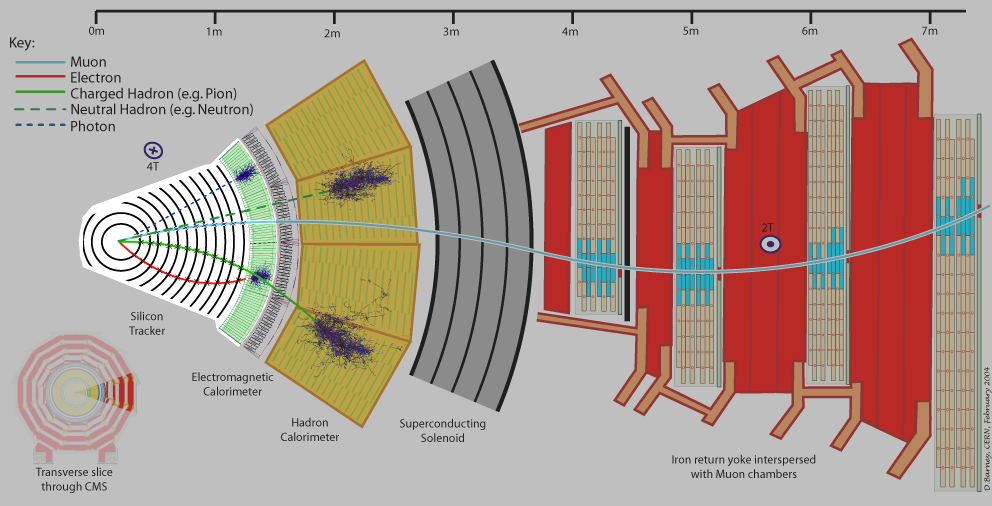
\includegraphics[width=0.75\textwidth]{figures/flowOfParticlesThroughCMS.png}
	\caption{Typical trajectories of particles travelling through CMS, from CERN.}
	\label{fig:particleTrajectories}
\end{figure}


\section{Track Reconstruction}
\label{sec:trkReco}
Charged particles are reconstructed as helical tracks from signals measured in the silicon tracker.  An interative algorithm 
starts by reconstructing tracks from signals in the inner pixel tracker characterized by the highest energies or smallest 
distances from the IP, and progressively includes signals measured in outer pixel tracker and silicon strip tracker layers.  
Signals in successive layers are linked into continuous tracks using a Kalman filter that requires each signal to have 
$\chi^{2} <$ 30 \cite{trackerPerformanceInCollisions}.  Each time a new signal is added to a track, an analytic function 
extrapolates the track trajectory to the next layer assuming energy is lost only through ionization in the silicon.  Hits in 
the next layer are searched for in the region identified by the analytic function extrapolation, and this procedure repeats 
until signals are included from the outermost silicon strip tracker layer.  Then, the signals linked into tracks are removed 
from the list of track candidates, and the algorithm restarts using signals measured in the inner pixel tracker characterized 
by lower energies or larger distances from the IP.  Using this algorithm, isolated muons with $\pt > 0.9$ $\GeV$ and $|\eta| < 2.4$ 
were reconstructed as tracks with essentially 100\% efficiency \cite{trackerPerformanceInCollisions}.  After reconstructing 
all tracks in an event, each point where two or more tracks originate is identified as an interaction vertex, and its position 
is measured relative to the IP.  The positions of vertices that have muon tracks with $|\eta| < 1.4$ and $\pt = 100$ $\GeV$ 
were measured with 10 and 30 $\mu$m resolutions in the transverse (r-$\phi$) and longitudinal ($z$) directions.

The track reconstruction algorithm described previously is used to reconstruct muon and charged hadron tracks, but a second 
algorithm is used to reconstruct electron tracks.  The silicon tracker contains, depending on $\eta$, 1 to 2 radiation 
lengths of material that causes electrons to shower.  As a result, $\sim$35\% of electrons that traverse the tracker lose more 
than 70\% of their initial energies through bremsstrahlung \cite{trackerPerformanceInCollisions}, which cannot be measured by 
the tracker.  The electron track reconstruction algorithm uses the same iterative track reconstruction procedure described 
previously, but extrapolates each track's trajectory to the next silicon layer assuming the energy lost through bremsstrahlung 
is described by a sum of Gaussians.  In addition, the Kalman filter used to link signals in successive layers requires that new 
signals have $\chi^{2} <$ 2000.  The electron track algorithm reconstructed electrons that had $\pt > 20$ $\GeV$ and $|\eta| < 2.5$ 
as tracks with 97\% or better efficiency \cite{gsfPerformanceInCollisions}.


\section{Energy Reconstruction}
\label{sec:enrgReco}
The energies of photons, electrons, and hadrons produced by pp interactions are measured in groups of ECAL crystals.  Photons, 
electrons, and hadrons impinging on the ECAL generate signals in the ECAL crystals that are converted into uncalibrated energies.  Groups, 
or superclusters (SCs), of crystals are built from the most energetic crystals with $\Et \gtrsim 0.2$ $\GeV$ and their nearest 
neighbors, and are at least 3 crystals wide in $\eta$.  The upstream tracker material causes $\sim$35\% of electrons and 
photons, and up to 25\% of hadrons \cite{trackerPerformanceInCollisions} to shower in the tracker, and radiate energy by emitting 
photons and other particles.  The energy is typically radiated along the particle's $\eta$ trajectory, but spread over several ECAL 
crystals in $\phi$.  To capture this energy, each SC is at least 5 crystals wide in $\phi$, and can be much larger, as in 
Figure \ref{fig:eleTrackAndSC}.  Once a SC is built, the energy of each crystal in the SC is multiplied by a laser 
transparency correction, and relative and absolute energy calibration corrections.  The sum of the calibrated crystal energies 
is the SC energy, and the energy weighted average $(\eta,\phi)$ position is the SC position.  Using only ECAL SCs, the $(\eta,\phi)$ 
positions of electrons in the barrel (endcap) were measured with a $\phi$ resolution of 0.17$^{\circ}$ (0.29$^{\circ}$), and an 
$\eta$ resolution of 0.001 (0.002) units.

The energies of hadrons that traverse the ECAL are measured in groups of HCAL towers.  Hadrons impinging on the HCAL generate signals 
in the HCAL towers that are converted into uncalibrated energies.  The highest energy towers with $\Et \gtrsim 1$ $\GeV$ are used to 
seed clusters, which extend to all neighboring towers with $\Et > 0.8$ $\GeV$ \cite{pflowEventReco}.  If one tower is grouped into 
multiple clusters, the tower's contribution to each cluster is weighted by its distance from each cluster's seed.  After clusters are 
built, each tower's energy is multiplied by a laser transparency correction, and relative and absolute energy calibration corrections.  
The sum of the calibrated tower energies is the cluster energy, and the energy weighted average $(\eta,\phi)$ position is the cluster 
position.  Hadron energies are measured as a combination of calibrated HCAL cluster energies, and energies of overlapping ECAL SCs.  
Using the combined ECAL-HCAL system, hadrons with $\Et = 100$ $\GeV$ were measured with a $\sim$10\% $\Et$ resolution \cite{pflowEventReco}.


\section{Muon Reconstruction and Selection}
\label{sec:muReco}

\subsection{Reconstruction}
Muons are first reconstructed as tracks from signals measured in individual muon chambers.  In each DT chamber, the start and end points of 
track segments are identified first as pairs of signals measured in the same plane (r-$\phi$ or r-z) but in different layers.  Then straight 
lines are drawn between the signal pairs, and a signal pair is ignored if its line is not compatible with a track that extrapolates from 
the chamber to the IP.  The remaining signals that are consistent with any of these straight lines are built into track segments that are 
measured in at least 3 layers.  In each plane the track segment with signals in the largest number of layers, at least 3, and the lowest 
$\chi^{2}/nDOF$, less than 20, is used to build a 3D track.  In the event where more than one track segment is reconstructed 
in one plane of a DT chamber, all combinations of r-$\phi$ and r-z track segments are considered when reconstructing a 3D track.  In 
practice, more than one 3D track is reconstructed in a DT chamber in less than 1\% of events \cite{cmsTdrPhysPerformance}.  The same 
track segment reconstruction algorithm is used in each 6 layer, single plane CSC.  There the final track segment must have signals 
in at least 4 layers.  In the barrel-endcap transition region, $1.3 < |\eta| < 1.6$, where the DT chambers stop and the CSCs begin, RPCs 
are used to improve the muon reconstruction efficiency and the precision of arrival time measurements.  Each RPC contains two parallel 
plates divided into many thin strips, and strips that measure a signal are grouped into clusters.  Each reconstructed cluster represents 
a hit whose position is the 'center of gravity' of all the strips in the cluster.

Tracks reconstructed in individual chambers are used to reconstruct muon trajectories through the magnetic field and all muon chambers.  
A Kalman filter algorithm starts with tracks in the chambers closest to the IP, and predicts the track positions in chambers in the next 
radial station with the effects of an inhomogeneous magnetic field and material losses taken into account \cite{muonRecoFirstCollisions}.  
Track segments in outer chambers are added to existing tracks subject to a $\chi^{2}$ requirement, and existing tracks are propagated to 
the next radial station even if no matching track segment is found in the current station.  Once the outermost station is included, a 
reverse Kalman filter is applied to reconstructed tracks from the outermost station working to the innermost station.  The reverse Kalman 
filter finalizes the track parameters, then these tracks are compared to silicon tracker tracks to identify global muons.

Global muons are identified using tracks reconstructed in the silicon tracker and muon detectors.  Tracks from the muon detectors are 
extrapolated back to the outermost silicon tracker layer, and their positions are compared.  In the local coordinate plane of the 
silicon strip layer, each silicon tracker track that matches a muon detector track within 3 cm is identified as a global muon.  If an 
extrapolated muon detector track has multiple silicon tracker track candidates within 3 cm, the closest match is used to make a global 
muon.  The matched silicon tracker track determines the $(\eta,\phi)$ trajectory of each global muon.

The momentum of each global muon is determined by sampling four different global muon reconstruction algorithms, and selecting the  
highest quality result.  Each algorithm fits a continuous track \cite{cmsMuonRecoRunTwo} to a unique combination of silicon tracker 
and muon detector signals to estimate a muon's trajectory through CMS, depicted in Figure \ref{fig:particleTrajectories}.  The 
quality of each continuous track is identified by a fit uncertainty $\chi^{2}/nDOF$ and momentum uncertainty $\sigma(\pt)/\pt$; and 
the track with the lowest $\chi^{2}/nDOF$ and momentum uncertainty $\sigma(\pt)/\pt < 0.3$ determines the global muon's momentum.  
For muons with $\pt \lesssim 100$ $\GeV$ the highest quality result is obtained using only silicon tracker measurements.  Muons with 
$|\eta| < 1.4$ and $\pt = 100$ $\GeV$ were measured with a $\pt$ resolution of $\sim$2.8\% \cite{trackerPerformanceInCollisions}.  
However, as a muon's $\pt$ increases above 100 $\GeV$ the silicon tracker $\pt$ resolution degrades faster that that of the muon 
detectors.  A significant fraction of $\WR \rightarrow \mu\mu jj$ events are expected to produce at least one muon with $\pt > 200$ $\GeV$ 
(Table \ref{tab:wrHighPtMuons}), and in this high $\pt$ region the highest quality momentum measurement is made by combining silicon 
tracker and muon detector measurements.  Muons with $|\eta| < 0.9$ and $200 < \pt < 400$ $\GeV$ were measured with a $\pt$ resolution 
of 3.2\%, and higher $\pt$ muons were measured with a resolution better than 6\% \cite{cmsMuonRecoRunTwo}.

\begin{table}[h]
	\caption{Fraction of expected $\WR \rightarrow \mu\mu jj$ events that had at least one muon with $\pt > 200$ $\GeV$. 
	($\mnul = \frac{1}{2}\mWR$)}
	\label{tab:wrHighPtMuons}
	\centering
	\begin{tabular}{c|c}
		\mWR ($\TeV$) & Fraction of events with at least one high-$\pt$ muon (\%) \\  \hline
		1.0 &  80.  \\
		2.0 &  95.  \\ 
		3.0 &  98.  \\ \hline
	\end{tabular}
\end{table}

Global muons reconstructed in simulated events have different energies than muons reconstructed in data.  Energy 
corrections for simulated muons are derived using $Z \rightarrow \mu\mu$ events found in simulations and data.  The di-muon mass 
($M_{\mu\mu}$) distribution in $Z \rightarrow \mu\mu$ events is compared between data and simulations, and the energies of muons 
in simulated events are corrected so that the two $M_{\mu\mu}$ distributions match.

\subsection{Online Selection}
\label{sec:muOnlineSel}
\WR decays that produce two muons can be selected online using single muon or double-muon triggers.  The single muon 
triggers require one track segment to be reconstructed in multiple muon detectors and have $\pt$ above some threshold $A$, while the 
double-muon triggers require two track segments that have $\pt$ above some threshold $B < A$.  In simulated $\WR \rightarrow \mu\mu jj$ events the 
highest efficiency single muon trigger selected more \WR events than the highest efficiency double muon trigger (Table \ref{tab:singleVsDblMuHlt}).  
Although the double-muon trigger $\pt$ selection criteria were lower than those of the single muon trigger, the double-muon trigger 
selected fewer \WR events because the efficiency to reconstruct a muon with $\pt > B$ as a track segment was below 100\% \cite{cmsMuonRecoRunTwo}.  
To maximize the trigger efficiency a single muon trigger was used to select collision events with muons.

\begin{table}[h]
	\caption{The efficiency of a single and double-muon trigger in simulated $\WR \rightarrow \mu\mu jj$ events with $\mWR = 800$ $\GeV$ 
		and $\mnul = 400$ $\GeV$.}
	\label{tab:singleVsDblMuHlt}
	\centering
	\begin{tabular}{c|c}
		trigger $\pt$ criteria & efficiency (\%) \\  \hline
		one $\mu$ $\pt >50$ $\GeV$ & 98  \\ 
		one $\mu$ $\pt >17$, another $\mu$ $\pt >8$ $\GeV$ & 93  \\
	\end{tabular}
\end{table}

During collisions events with muons were selected using a Level-1 trigger that required one track segment with $\pt > 16$ $\GeV$.  The 
segment was required to have signals in DT or CSC chambers from at least 2 stations, and signals in at least 4 layers of each chamber.  
Then, events were required to pass the following single muon HLT selection criteria:

\begin{itemize}
	\item A track reconstructed in the silicon tracker with $\pt > 50$ $\GeV$ and $|\eta| < 2.4$ was geometrically matched to 
		the muon detector track segment that passed the L1 trigger.
	\item In the plane perpendicular to the beam axis, the distance between the silicon tracker track origin and its 
		reconstructed vertex was $< 1$ mm.
\end{itemize}

Simulated muons pass the trigger criteria with a different efficiency than muons produced in real collisions.  This 
efficiency difference was corrected by multiplying the weight of every simulated event (default weight is 1.0) by a $\pt$,$\eta$-
dependent value between 0.95 (5\% decrease) and 1.04 (4\% increase) for the muon that fired the trigger.

\subsection{Offline Identification Selection}
In events selected by the single muon trigger, muons were reconstructed offline from tracks in the muon detectors and silicon tracker using 
algorithms described previously.  Then, the following identification criteria were applied to select promptly produced muons 
that were isolated from other particles and reconstructed in multiple muon stations:

\begin{itemize}
	\item The muon track reconstructed in the silicon tracker:
	\begin{itemize}
		\item Was reconstructed from a signal in at least 1 silicon pixel detector layer, and signals in at least 
			5 layers in the entire tracker.
		\item Within a cone of radius $\Delta R = 0.3$ centered on the track, the $\sum \pt$ of all other 
			reconstructed tracks was low compared to the muon $\pt$, $\frac{\sum \pt}{\mu \pt} < 0.1$.
	\end{itemize}
	\item The muon's track segment went through a muon chamber in at least 2 muon stations.  Track segments in each DT 
		chamber were required to have signals in all 4 r-$z$ layers, and at least 7 of 8 r-$\phi$ layers.  Track segments 
		in each CSC were required to have signals in all 6 layers.
	\item The origin of the muon's silicon tracker track was within 2 mm of the muon's reconstructed vertex 
		position along the $z$ axis.
\end{itemize}

Simulated muons are reconstructed and pass the offline muon identification selection criteria with a higher 
efficiency than muons produced in real collisions.  This efficiency difference was corrected by multiplying the weight of every 
simulated event by a $\pt$,$\eta$-dependent value between 0.985 and 1.0 for each offline muon selected in the event.


\section{Electron Reconstruction and Selection}
\label{sec:eleReco}

\subsection{Reconstruction}
Electrons are the only particles from \WR decays expected to lose more than a few percent of their initial energy through 
bremsstrahlung in the tracker.  A dedicated electron track reconstruction algorithm is used to reconstruct tracks from electrons, 
even those that experience large energy losses, with high efficiency, but the tracker cannot measure the magnitude of bremsstrahlung 
energy losses.  However, the energies of electrons and their bremsstrahlung photons are measured by the ECAL.  Therefore, the ECAL 
is used to measure the $\Et$ and $(\eta,\phi)$ trajectory of each electron.

Electrons are identified using reconstructed tracks and ECAL SCs.  Reconstructed tracks are extrapolated from the outermost 
silicon strip layer to the front face of the ECAL, and their positions are compared to ECAL SCs.  Each electron is identified 
as one or more tracks that match the SC $(\eta,\phi)$ position within 1.1$^{\circ}$, about 1 crystal wide, in $\phi$, and 
within 0.004 units, less than $\frac{1}{2}$ a crystal wide, in $\eta$.  In addition, the ECAL SC $\Et$ and the matched 
track(s) $\pt$ must agree within the uncertainty on the track $\pt$.  Using the SC energy, electrons with $\Et \approx 45$ 
$\GeV$ and $|\eta| < 0.8$ were measured with an $\Et$ resolution better than 2\%, and a resolution between 2\% and 5\% 
at higher $|\eta|$ \cite{ecalPerformanceInCollisions}.

\begin{figure}[h]
	\centering
	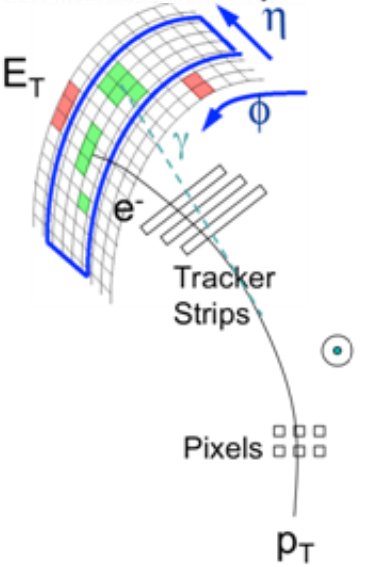
\includegraphics[width=0.75\textwidth]{figures/electronTrackAndSupercluster.png}
	\caption{The trajectory of a typical electron through the tracker and the ECAL.}
	\label{fig:eleTrackAndSC}
\end{figure}

Electrons reconstructed in simulated events have different energies than electrons reconstructed in data.  Energy 
corrections for simulated electrons are derived using $Z \rightarrow ee$ events found in simulations and data.  The di-electron mass 
($M_{ee}$) distribution in $Z \rightarrow ee$ events is compared between data and simulations, and the energies of electrons 
in simulated events are corrected so that the two $M_{ee}$ distributions match.

\subsection{Online Selection}
\WR decays that produce two electrons can be selected online using single electron or double-electron triggers.  The single electron 
triggers require that one track reconstructed in the silicon tracker extrapolates to a 5 $\times$ 5 ECAL crystal region with $\Et$ above some 
threshold $D$, while the double-electron triggers require two such track-ECAL cluster combinations each with $\Et$ above some threshold 
$G < D$.  In simulated $\WR \rightarrow eejj$ events the highest efficiency single and double-electron triggers selected similar numbers 
of signal events (Table \ref{tab:singleVsDblEleHlt}), so a trigger was chosen for another reason.  The electron trigger was used 
to select signal events and events in a low dilepton mass ($\Mll$) control region discussed later.  The low $\Mll$ control region was 
used to estimate the $\DY$+jets background, and needed as many $\DY$+jets events as possible to minimize the statistical uncertainty 
on the background estimate.  The single electron trigger required $\Et > 105$ $\GeV$, and excluded a significant fraction of 
$Z \rightarrow ee$ events.  To select a larger portion of $Z \rightarrow ee$ events, the double-electron trigger, which required two 
electrons to have $\Et > 33$ $\GeV$, was used to select collision events with electrons.

\begin{table}[h]
	\caption{The efficiency of a single and double-electron trigger in simulated $\WR \rightarrow \mu\mu jj$ events with $\mWR = 800$ $\GeV$ 
		and $\mnul = 400$ $\GeV$.}
	\label{tab:singleVsDblEleHlt}
	\centering
	\begin{tabular}{c|c}
		trigger $\Et$ criteria & efficiency (\%) \\  \hline
		one $e$ $\Et >105$ $\GeV$ & 94  \\ 
		two $e$ $\Et >33$ $\GeV$ & 92  \\
	\end{tabular}
\end{table}

During collisions events with electrons were selected using single and double-electron Level-1 triggers.  These triggers required 
one 5 $\times$ 5 ECAL crystal cluster that had $\Et > 40$ $\GeV$, or two 5 $\times$ 5 ECAL clusters that had 
$\Et > 22$ $\GeV$ and $\Et > 10$ $\GeV$.  Then, events were required to pass the following double-electron HLT selection criteria:

\begin{itemize}
	\item Two 5 $\times$ 5 ECAL crystal clusters separated by $\Delta R > 0.1$ were required to have $\Et > 33$ $\GeV$.
	\item For each ECAL cluster with energy E:
	\begin{itemize}
		\item The hadronic energy behind the cluster was $<$ 15\% of E in the barrel, and $<$ 10\% of E in the endcap. 
		\item Ninety percent of E was measured in an area that was two crystals wide in $\eta$.
		\item If the cluster was in the barrel, a reconstructed track with signals in at least two pixel tracker layers 
			extrapolated close to the cluster position.  The track extrapolated from the pixel tracker to within $2.3$ cm 
			of the cluster $z$ position, and to within 1 ECAL crystal area of the cluster $(\eta,\phi)$ position.
	\end{itemize}
\end{itemize}

Simulated electrons passed the trigger criteria with the same efficiency as electrons produced in real collisions, so no electron 
trigger efficiency correction was applied to simulated events.

\subsection{Offline Identification Selection}
In events selected by the double-electron trigger, electrons were reconstructed offline from ECAL SCs and tracks using algorithms 
described previously.  Then, the following identification criteria were applied to select promptly produced 
electrons that did not lose significant energy in the tracker, and were not reconstructed from a real jet, or in the ECAL barrel-endcap 
transition region $1.44 < |\eta| < 1.57$:

\begin{itemize}
	\item The electron $\Et$ is the calibrated ECAL SC energy $E_{SC}$.
	\item For a SC in the barrel, at least 94\% of $E_{SC}$ was measured in an area that was 2 crystals wide in $\eta$.
	\item The hadronic energy (H) behind the SC was $\frac{H}{E_{SC}}< 0.05 +\thickspace \frac{1 \GeV}{E_{SC}}$ 
		in the barrel, and $\frac{H}{E_{SC}}< 0.05 +\thickspace \frac{5 \GeV}{E_{SC}}$ in the endcap.
	\item In a $\Delta R =$ 0.3 radius cone centered on the electron's $(\eta, \phi)$ trajectory:
	\begin{itemize}
		\item The $\sum \pt$ of all tracks excluding the electron's track was low, $\sum \pt < 5$ $\GeV$.
		\item The total calorimeter energy $E_{ECAL + HCAL}$ not associated with the electron was 
			$E_{ECAL + HCAL} < 2 + 0.03\alpha + 0.28\rho$.  $\rho$ is the neutral particle energy per unit $\eta,\phi$ area, 
			$\alpha$ in the barrel is $E_{SC}$, and $\alpha$ in the endcap is $E_{SC} - 50$.
	\end{itemize}
	\item For a SC in the endcap, the electron track extrapolated from the outermost silicon tracker measurement to the SC 
		seed crystal position to within $\sim$3 crystal widths in $\phi$.
	\item The electron track was reconstructed from signals in every silicon pixel and inner strip detector layers, or all but 1 layer.
	\item The electron track's origin was separated from its vertex by a small distance $\Delta_{xy}$ in the $x-y$ 
		plane: $\Delta_{xy} < 0.2$ mm in the tracker barrel, and $\Delta_{xy} < 0.5$ mm in the tracker endcap.
\end{itemize}

Simulated electrons are reconstructed and pass the offline electron identification selection criteria with a higher 
efficiency than electrons produced in real collisions.  This efficiency difference was corrected by multiplying the weight of every 
simulated event by 0.982, the reconstruction efficiency correction, and by 0.989, the ID efficiency correction, for each offline 
electron selected in the event.


\section{Jet Reconstruction and Selection}
\label{sec:jetReco}

\subsection{Reconstruction}
Quarks and gluons emitted from pp interactions produced jets of photons, hadrons and leptons.  On average, 85\% of a jet's 
energy is carried by charged particles and photons \cite{pflowJetRecoInCollisions}, so these particles are reconstructed first during 
jet reconstruction.  The particle flow jet reconstruction algorithm \cite{pflowEventReco} identifies $(\eta,\phi)$ regions 
with one or more silicon tracker or muon detector tracks, one or more HCAL energy clusters, and any number of ECAL 
SCs.  In these regions, algorithms described previously are used to reconstruct muons first, followed by electrons.  Tracks and 
energy deposits identified as leptons are subsequently removed from the list of particle candidates.  The remaining tracks and energy clusters 
are used to identify charged hadrons, photons, and neutral hadrons.  Each charged hadron is identified as a track that extrapolates to 
an HCAL cluster and possibly an ECAL SC.  The charged hadron's $\pt$ and $(\eta,\phi)$ trajectory are determined by the track, and the track 
$\pt$ must agree with the total calorimeter $\Et$ within the calorimeter $\Et$ uncertainty.  Each photon is identified as an ECAL SC 
that is not geometrically matched to a track or HCAL cluster whose $\pt$ or $\Et$ agrees with the SC $\Et$ within the ECAL $\Et$ 
uncertainty.  The energy matching criteria is critical to reconstructing photons in close proximity to other particles in jets.  
Finally, each neutral hadron is identified as an HCAL cluster and any overlapping ECAL SC that are not geometrically 
matched to a track whose $\pt$ agrees with the calorimeter $\Et$ within the calorimeter $\Et$ uncertainty.  After all tracks and 
energy clusters in a region are identified as specific particles, a jet, represented by the cone in Figure \ref{fig:jetClustering}, 
is clustered from those particles.

Due to the high instantaneous collision luminosity, each pp bunch crossing delivered by the LHC produces multiple pp interactions, 
or pileup (PU) interactions, that make jet clustering more challenging.  In every unit of $\eta$, each PU interaction adds 
$\sim$11 charged particle tracks with $\pt \approx 0.5$ $\GeV$ to the event \cite{chgdHdrMultInData}.  These tracks are primarily 
charged hadrons, so before jets are clustered the charged hadrons associated with PU interaction vertices are removed from 
all jet clustering regions.  Jets are then clustered from reconstructed particles using the anti-$k_{T}$ algorithm \cite{antikt} 
with a distance parameter $R = 0.4$.  In each region the anti-$k_{T}$ algorithm starts with the highest $\pt$ hadron and adds 
other particles to the jet based on their $\pt$ and distance from the jet axis.  Using the distance parameter $R = 0.4$, 
particles located $\Delta R > 0.4$ from the jet axis are less likely to be clustered into the jet than particles located within 
$\Delta R \leq 0.4$.  Once anti-$k_{T}$ jets are clustered a second set of smaller jets are clustered to estimate the average 
increase in jet energy due to neutral particles produced in PU interactions.  The second set of jets are clustered from 
reconstructed particles using the $k_{T}$ algorithm \cite{ktAlgoOne,ktAlgoTwo,ktAlgoThree} with distance parameter $R = 0.3$.  
Then each $k_{T}$ jet's $\pt$ is divided by its area ($\pt_{j} / A_{j}$), and the median value $\rho$ is the average neutral 
particle energy density in the event \cite{pileup1,pileup2}.  Each PU interaction increases $\rho$ by about 0.5 $\GeV$ 
\cite{jetResolutionInCollisions}.  Using the hybrid jet area subtraction technique described in \cite{pflowJetRecoInCollisions}, 
the photon and neutral hadron energies in each anti-$k_{T}$ jet are reduced by multiplying $\rho$ by the jet's area and and $\eta$ 
dependent factor.  After the area based subtraction, jet energies are calibrated to correct for known $\eta$ and $\pt$ variations 
of the detector's response to jets.  After calibrations, particle flow jets with $\pt > 40$ $\GeV$ and $|\eta| < 1.3$ were 
measured with a $\pt$ resolution of 16\% or better \cite{jetResolutionInCollisions}.

\begin{figure}[h]
	\centering
	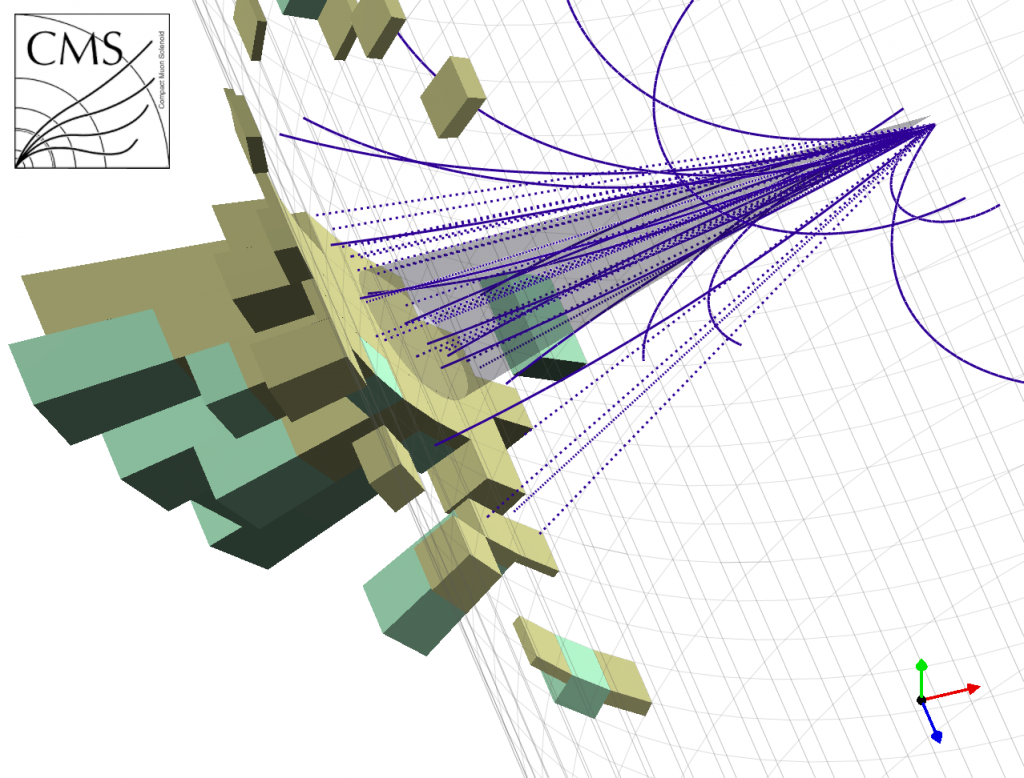
\includegraphics[width=0.75\textwidth]{figures/jetClusteringInCMS.png}
	\caption{A cone of reconstructed particles clustered into a jet, with the reconstructed vertex on the right.  
	From the CMS Experiment.}
	\label{fig:jetClustering}
\end{figure}

Jets reconstructed in simulated events have different energies than jets reconstructed in data.  Energy corrections for 
simulated jets are derived using dijet, $Z$+jet, and $\gamma$+jet events found in simulations and data 
\cite{jetpaper}.  The di-jet mass and leading jet $\pt$ distributions in these events are compared between data and simulations, and 
the energies of jets in simulated events are corrected so that the jet distributions match in data and simulations.

\subsection{Offline Identification Selection}
In events selected by the single muon or double-electron trigger, jets were reconstructed offline from tracks and calorimeter energy 
clusters using algorithms described previously.  Then, the following identification criteria were applied to select 
jets that contained at least one charged hadron, and whose energies were not dominated by ECAL SCs not linked to HCAL clusters:

\begin{itemize}
	\item The jet had at least 2 constituents.
	\item The jet had at least 1 charged hadron constituent.
	\item More than 0\% of the total jet energy came from charged hadrons.
	\item Less than 90\% of the total jet energy came from neutral hadrons.
	\item Less than 90\% of the total jet energy came from photons.
	\item Less than 99\% of the total jet energy came from electrons.
\end{itemize}

Simulated jets are reconstructed and pass the ID criteria with the same efficiency as jets produced in real collisions, so no jet 
reconstruction or ID efficiency corrections were applied to simulated events.


\section{\WR Signal and ST Backgrounds Kinematics}
\label{sec:signalAndBkgnds}
The online and offline ID selection criteria were used to select events where two real leptons and hadronic jets were most likely produced, 
and created signals in the CMS detector that were correctly reconstructed as two leptons and two jets.  These selection criteria are 
equally applicable to any search for a new heavy particle that decays to leptons and jets \cite{exoLeptJetResults}, and are not optimized 
based on the kinematics of the \WR progeny.  The \WR decays to leptons and jets whose kinematics, like $\pt$ and dilepton mass $\Mll$, differ 
significantly from those of leptons and jets produced by ST backgrounds.  The origins of these differences, and the relative differences in 
background production rates are described here.

The heavy \WR decays through a lighter \nul to two leptons and two jets according to the following decay chain:

\begin{tikzpicture}[grow=right]
	\node (Wr) at (0,0) {$\WR \thickspace \rightarrow \thickspace \nul + \ell$};
	\node (Ar) at (0.75,-0.4) {$\searrow$};
	\node (Nl) at (1.25,-0.75) {$\ell jj$};
\end{tikzpicture} $\newline$
The previous \WR and \nul search \cite{cmsWRRunOneResults} excluded \WR production at 95\% CL for $\mWR < 3$ $\TeV$ and 
$90 \GeV \lesssim \mnul < \mWR$.  Thus the \WR and \nul lifetimes, inversely proportional to their masses, are expected to be very short.  
Therefore the \WR and \nul decay promptly to leptons, and quarks that hadronize into jets.

The majority of background events are produced by the $\DY$+jets process and processes with at least one top quark; the remaining events are 
produced by diboson (WW, WZ, ZZ), W+jets, and QCD multi-jet processes.  In 2015 collisions \DY interactions produced two same flavor leptons 
in CMS at a rate that peaked at $\sim$36 Hz for dilepton mass $\Mll \approx 90$ $\GeV$, and decreased rapidly for higher $\Mll$.  The \DY 
interaction occurs between two quarks, and at $\sqrt{s} = 13$ $\TeV$ the probability for either quark to radiate a parton, equal to the QCD 
coupling $\alpha_{QCD}$, is $\sim$0.1.  Thus, in $\alpha_{QCD}^{2} \sim$0.01 
$=$1\% of \DY interactions the initial quarks radiate two partons before interacting.  Unlike \DY, the top quark background, primarily 
$t\bar{t}$ and t+W, produces $\ell\ell jj$ final states without initial state parton radiation.  In 2015 collisions top quark processes 
produced two leptons and two jets at a rate of $\sim$0.5 Hz, similar to the peak \DY rate weighted by the 1\% probability to radiate two partons.  
The top quark background is also the only significant background that produces the $e\mu jj$ final state twice as often as same flavor $\ell\ell jj$ 
final states.  The ratio of same flavor to mixed flavor events is used to predict the top quark background, using methods described later.  
Amongst the remaining backgrounds, only WZ and ZZ production produce two leptons and two jets without initial state parton radiation.  In 2015 
collisions the ZZ and WZ processes produced two leptons and two jets at rates below 0.01 Hz, negligible with respect to the $\DY$+jets and 
top quark backgrounds.  The other backgrounds - $qq/qg/gg \rightarrow$ WW, W+jets, and QCD multi-jet - produce two leptons and two jets only 
when the interacting quarks or gluons radiate partons, or when real jets are incorrectly reconstructed as leptons.  These backgrounds were 
negligible relative to the $\DY$+jets and top quark backgrounds.

\subsection{Signal and Background Kinematics}
The kinematics of leptons and jets produced in \WR decays are governed by \mWR and the ratio $\mnul/\mWR$.  Based on previous searches \mWR is 
expected to be similar to 
the $\sqrt{s} = 13$ $\TeV$ collision energy.  Thus \WR bosons are expected to have low net momentum, so in the lab frame their progeny \nul 
and $\ell$ are emitted isotropically.  In addition, the leptons and jets are produced with high $\pt$ (Figure \ref{fig:wrLeptJetPts}) and 
low $|\eta|$ (Figure \ref{fig:wrLeptJetEtas}).  At a specific \mWR, the ratio 
$\mnul/\mWR$ affects how the total energy \mWR is split amongst the leptons and jets, and their $(\eta,\phi)$ trajectories.  As 
$\mnul/\mWR$ approaches 1 the $\ell_{1}$, from $\WR \rightarrow \ell_{1}\nul$, is emitted with lower average transverse energy; the 
$\ell_{2}$ and both jets, from $\nul \rightarrow \ell_{2}jj$, are emitted with higher average transverse energy.  Conversely, as 
$\mnul/\mWR$ approaches 0 the $\ell_{1}$ carries more energy, and the $\ell_{2}$ and both jets carry less energy.  These trends 
in lepton and jet transverse energies as a function of $\mnul/\mWR$ are shown in 
Figure \ref{fig:wrLeptQrkPtsVarMNu}.  Furthermore, as $\mnul/\mWR$ approaches 0 the \nul is emitted with larger momentum (Figure 
\ref{fig:hvyNuMomentumVarMNu}).  The \nul momentum is conserved in its decay, and as that momentum increases the $\ell_{2} jj$ system 
is preferentially emitted in the lab frame, or boosted, along the \nul $(\eta,\phi)$ trajectory.  The boost of the \nul decay products 
decreases the $\Delta R(\ell,j)$ separation between $\ell_{2}$ and both jets (Figure \ref{fig:wrDrLeptQrkVarMNu}).  Since the \nul recoils 
against $\ell_{1}$ to conserve the \WR momentum in $\WR \rightarrow \ell_{1}\nul$, the boost at low $\mnul/\mWR$ increases the angle 
between $\ell_{1}$ and $\ell_{2}$ (Figure \ref{fig:wrLeptAngleSepVarMNu}).  The $\ell_{1}\ell_{2}$ invariant mass ($\Mll$) increases 
with the angle between the leptons, so the boost at low $\mnul/\mWR$ also increases the $\Mll$ (Figure \ref{fig:wrMllVarMNu}).

%to draw a plot of the angle between the two leptons use this argument in TTree Draw within quotes, and multiplied by 180/3.1416
% TMath::ACos(1-( (TMath::CosH(etaEle[0]-etaEle[1]) - TMath::Cos(phiEle[0]-phiEle[1]))/(TMath::CosH(etaEle[0])*TMath::CosH(etaEle[1]))  ))

The \DY+jets process produces events where low $\pt$ jets, and low $\Mll$ lepton pairs are reconstructed.  Before 
producing the dilepton system via \DY, the interacting quarks radiate two partons.  These partons are radiated with a 
probability that is independent of $\phi$ and the angle $\theta$ relative to the beam axis, but decreases rapidly with $\pt$.  These 
partons recoil against the $Z/\gamma^{*}$ to conserve the initial quark system momentum, and are reconstructed as jets.  Due to 
the $Z$ boson resonance, the majority of \DY interactions produce lepton pairs that have $60 < \Mll < 120$ $\GeV$.  The $\Mll$ window 
constrains both leptons to have $15 \lesssim \pt \lesssim 60$ $\GeV$, and average $\pt \sim M_{Z}/2$.  Events where 
the $Z$ boson has significant momentum, or the $\gamma^{*}$ has significant energy yield higher $\pt$ leptons, but at a significantly 
lower rate.

Top quark processes produce bottom quarks and $W^{\pm}$ bosons that decay, and produce events where low $\pt$ leptons and jets 
are reconstructed.  The dominant contribution to the top quark background is the $t\bar{t} \rightarrow \ell\ell jj$ decay, where 
both $W$ bosons decay to a charged lepton via $W^{\pm} \rightarrow \ell\nu$.  Due to combinatorics the $e\mu$ final state 
is produced twice as often as the $ee$ or $\mu\mu$ final state.  The reconstructed charged leptons are constrained by the $W$ mass to 
have $15 \lesssim \pt \lesssim 50$ $\GeV$, and their $\pt$ distributions peak near $M_{W}/2$.  However, since they are produced 
independently their invariant mass $\Mll$ can be as high as the $t\bar{t}$ rest mass.  The reconstructed lepton-jet invariant mass 
($\Mlljj$) distribution found in $t\bar{t}$ events peaks below the $t\bar{t}$ mass because of the neutrinos from the $W$ decay.

The WZ and ZZ processes produce events where low $\pt$ jets, and low $\Mll$ leptons pairs are reconstructed.  WZ and ZZ pairs can be 
produced with one off-shell boson ($M_{Z^{*}} < 90$ $\GeV$), but their production rate is maximized when both bosons are 
produced on-shell.  In both processes one $Z$ decays to leptons via $Z \rightarrow \ell\ell$.  The majority of these lepton pairs are 
reconstructed with $60 < \Mll < 120$ $\GeV$, and each lepton's $\pt$ distribution spans $15 \lesssim \pt \lesssim 60$ $\GeV$ and peaks 
near $M_{Z}/2$.  The second $Z$ in ZZ, and the $W$ in WZ decay to quarks via $W/Z \rightarrow qq$.  The quarks are reconstructed as 
two jets whose dijet mass is consistent with the progenitor $W$ or $Z$ mass.  Similar to the leptons from the $Z$ decay, the $W/Z$ mass 
window constrains each jet's $\pt$ distribution to $15 \lesssim \pt \lesssim 50$ $\GeV$, and creates a peak in the $\pt$ distribution 
near half the progenitor boson mass.  Finally, the $W$ and $Z$ masses also constrain the reconstructed $\Mlljj$ distribution to below 
the diboson rest mass.

The $qq/qg/gg \rightarrow$ WW, W+jets and QCD multi-jet backgrounds produce events where low $\pt$ leptons and jets are reconstructed.  
WW production contributes to the $\ell\ell jj$ final states when both bosons decay to charged leptons via $W^{\pm} \rightarrow \ell\nu$, 
and the initial state quarks or gluons radiate partons that are reconstructed as two jets.  Additionally, WW pairs yield multi jet and 
lepton final states when one boson decays to a charged lepton, the other boson decays to two quarks, and the initial state quarks or gluons 
radiate additional partons.  These events contribute to $\ell\ell jj$ final states when the real lepton and two jets are correctly 
reconstructed, and one parton is incorrectly reconstructed as a second lepton.  Leptons and jets reconstructed from $W$ decay 
products are constrained by the $W$ mass to have $15 \lesssim \pt \lesssim 50$ $\GeV$, while radiated partons, reconstructed as jets or 
leptons, are emitted with decreasing probability at higher $\pt$.  The $qq/qg \rightarrow W \rightarrow \ell\nu$+jets process radiates 
partons from the initial state quarks or gluons, and produces one charged lepton.  W+jets events contribute to $\ell\ell jj$ final states 
when the charged lepton and two jets are correctly reconstructed, and one parton is incorrectly reconstructed as a second lepton.  The 
$\ell$ from the $W$ decay is constrained by the $W$ mass to have $15 \lesssim \pt \lesssim 50$ $\GeV$, and the radiated partons, 
reconstructed as jets or leptons, are emitted with decreasing probability at higher $\pt$.  The QCD multi-jet background contributes to 
$\ell\ell jj$ final states when at least 4 outgoing partons are produced, 2 are reconstructed as jets, and 2 are incorrectly reconstructed 
as leptons.  The outgoing partons, reconstructed as jets or leptons, are produced with a probability that decreases with $\pt$.

ST background events that passed the trigger selection criteria produced leptons and jets with $\pt$ distributions shown in Figure 
\ref{fig:bkgLeptJetPts}.

\begin{figure}
	\centering
	\begin{subfigure}[t]{2.4in}
		\centering
		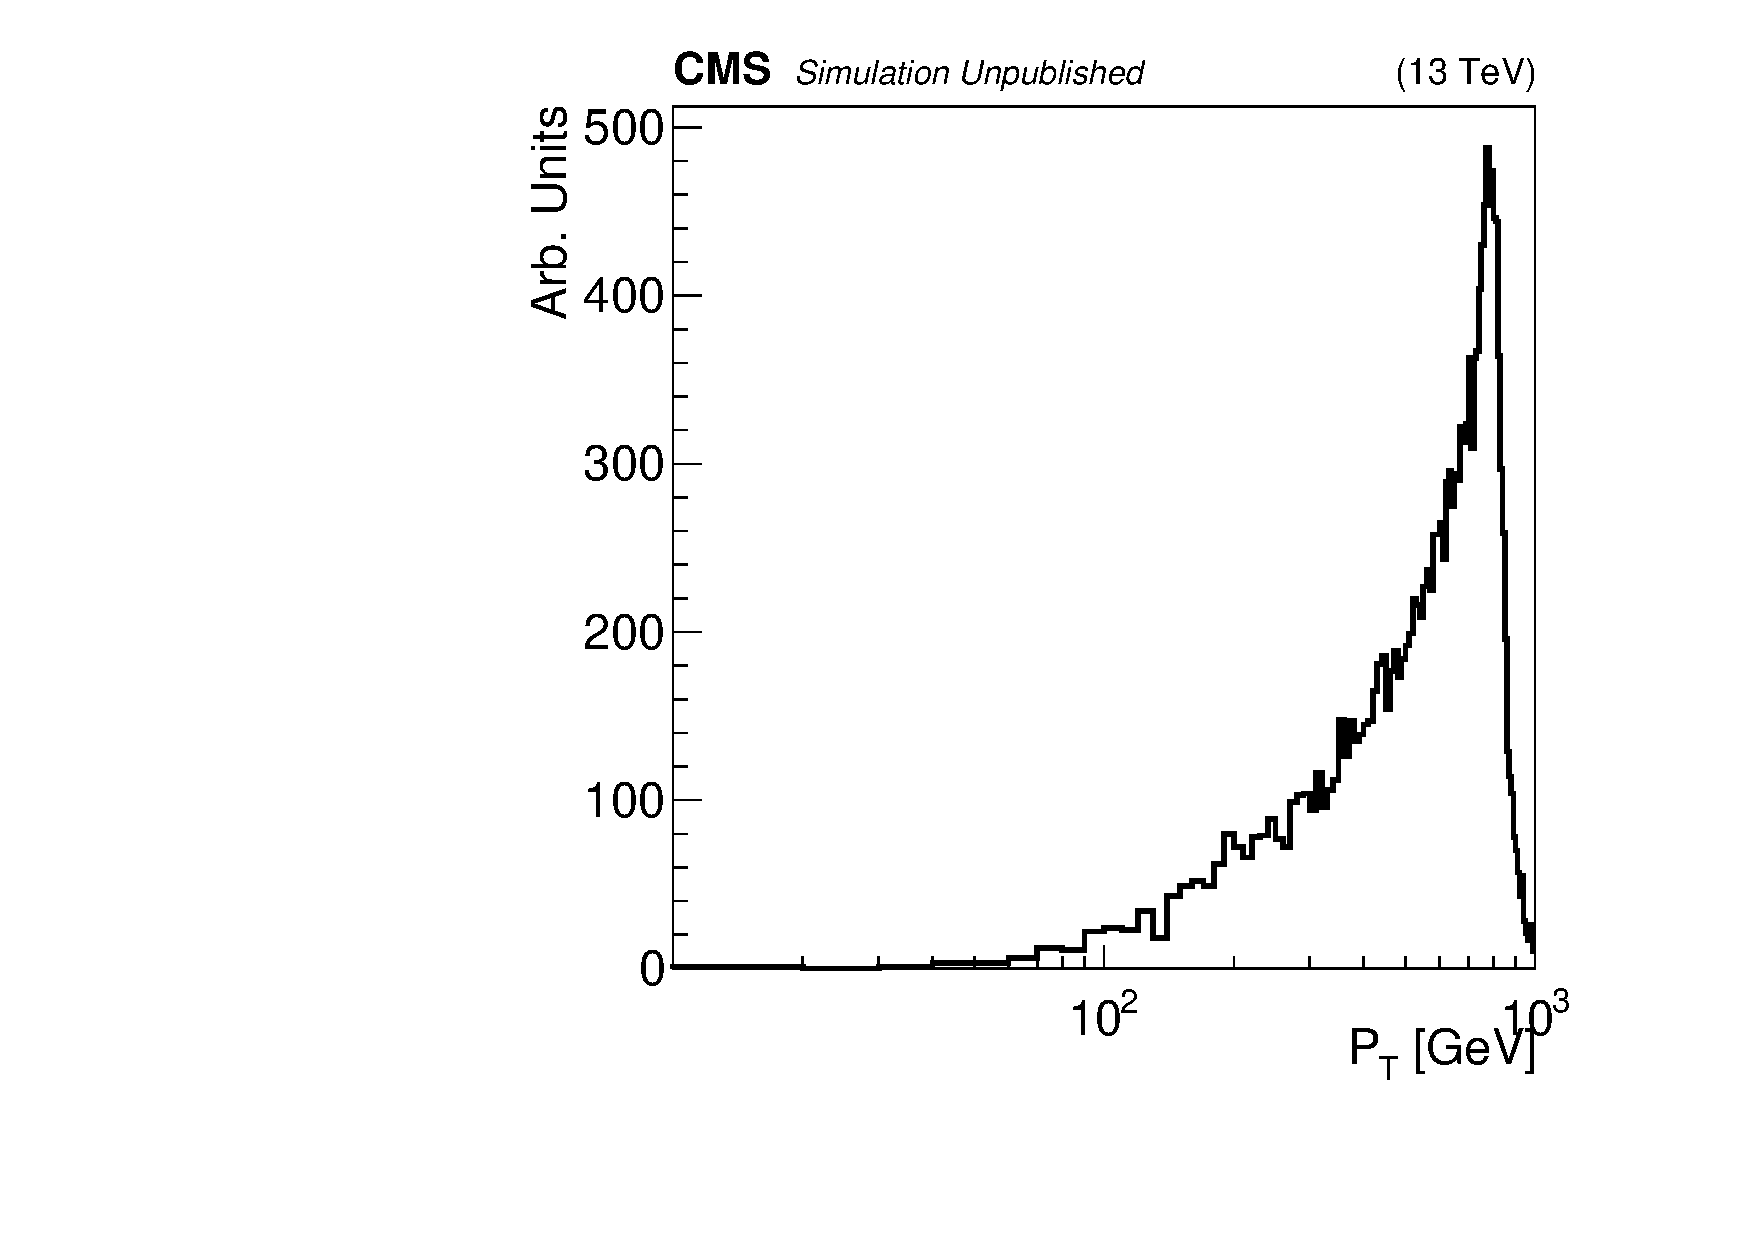
\includegraphics[width=2.4in]{figures/ptMatchedRecoEleFromWr_mwr2200_mnu1100.pdf}
		\caption{$\ell$ from $\WR \rightarrow \ell\nul$}\label{fig:wrLeptJetPtsa}
	\end{subfigure}
	\thickspace
	\begin{subfigure}[t]{2.4in}
		\centering
		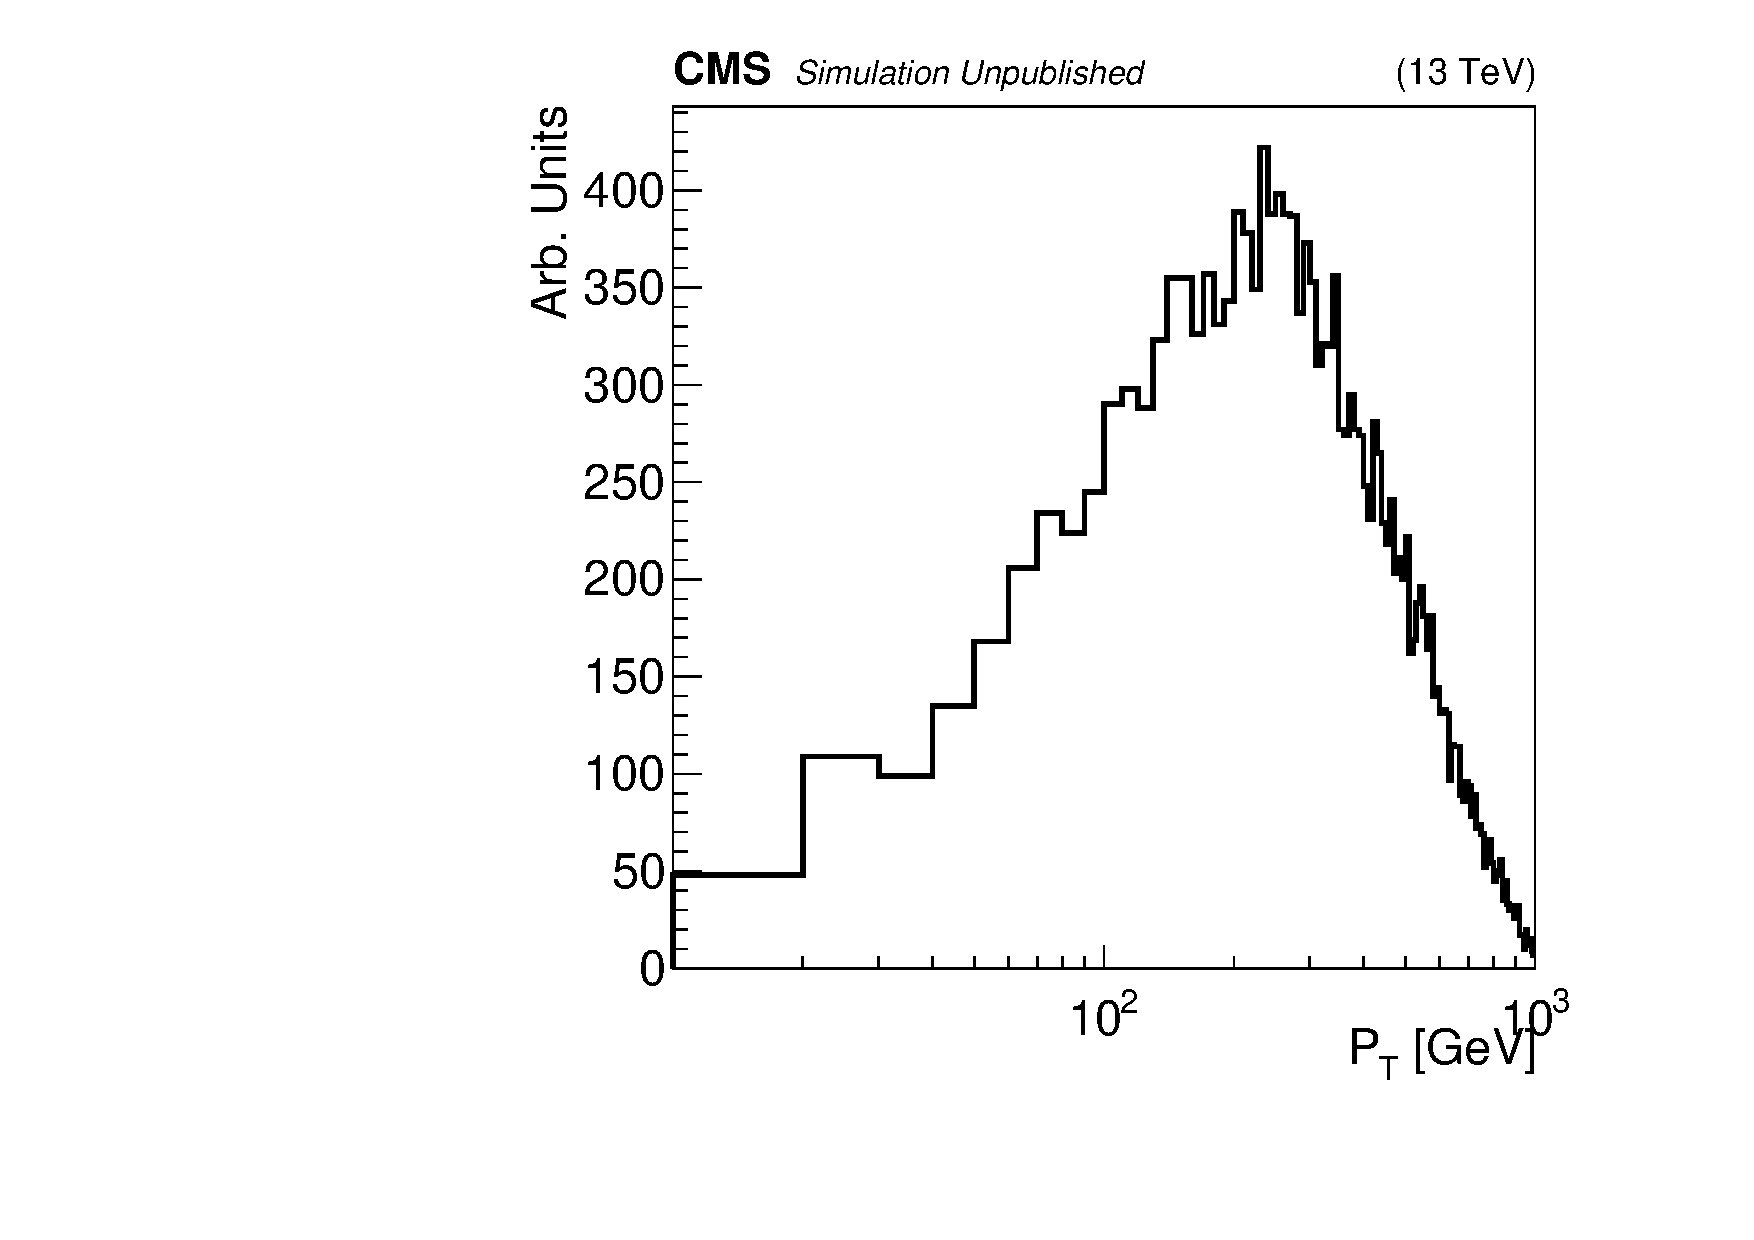
\includegraphics[width=2.4in]{figures/ptMatchedRecoEleFromNu_mwr2200_mnu1100.pdf}
		\caption{$\ell$ from $\nul \rightarrow \ell jj$}\label{fig:wrLeptJetPtsb}
	\end{subfigure}
	\newline
	\newline
	\newline
	\newline
	\begin{subfigure}[t]{2.4in}
		\centering
		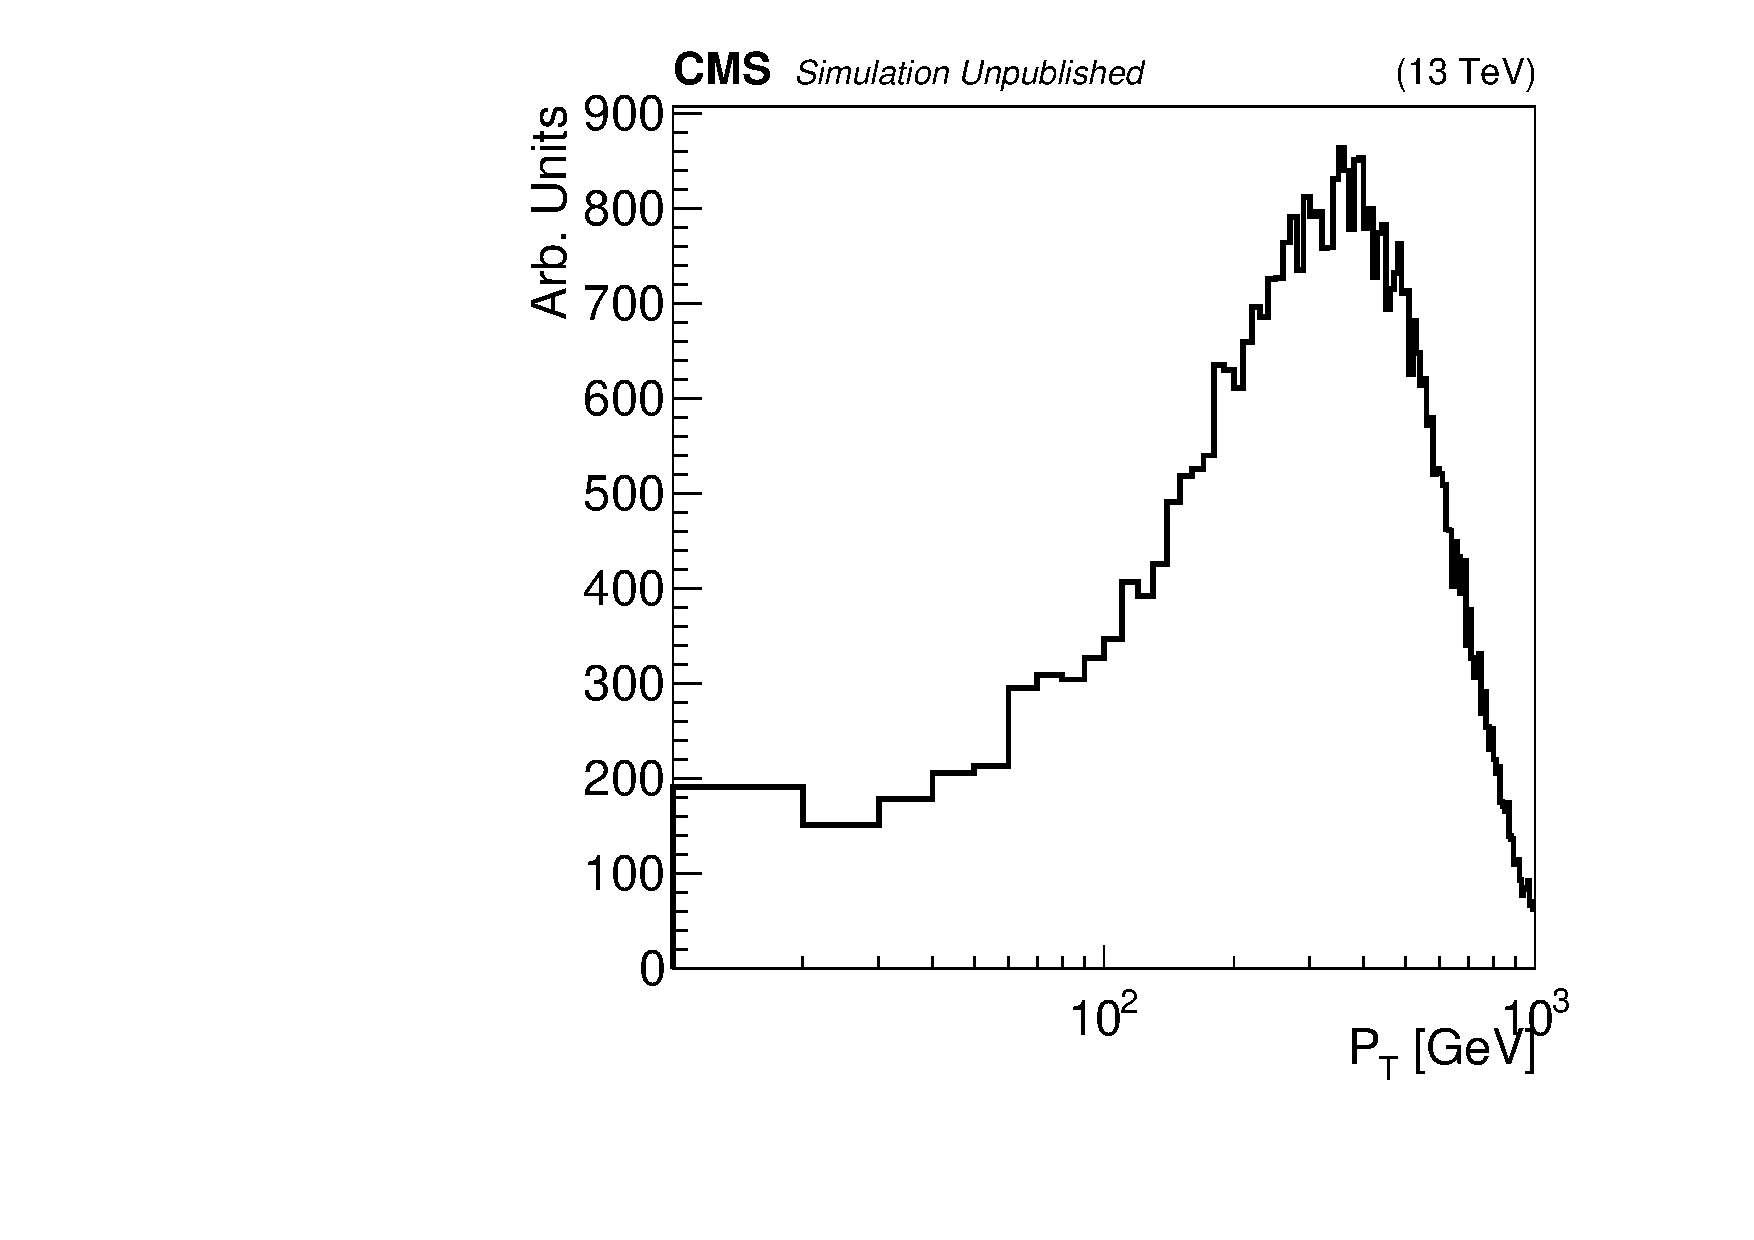
\includegraphics[width=2.4in]{figures/ptMatchedRecoJetOne_mwr2200_mnu1100.pdf}
		\caption{jet from $\nul \rightarrow \ell jj$}\label{fig:wrLeptJetPtsc}
	\end{subfigure}
	\thickspace
	\begin{subfigure}[t]{2.4in}
		\centering
		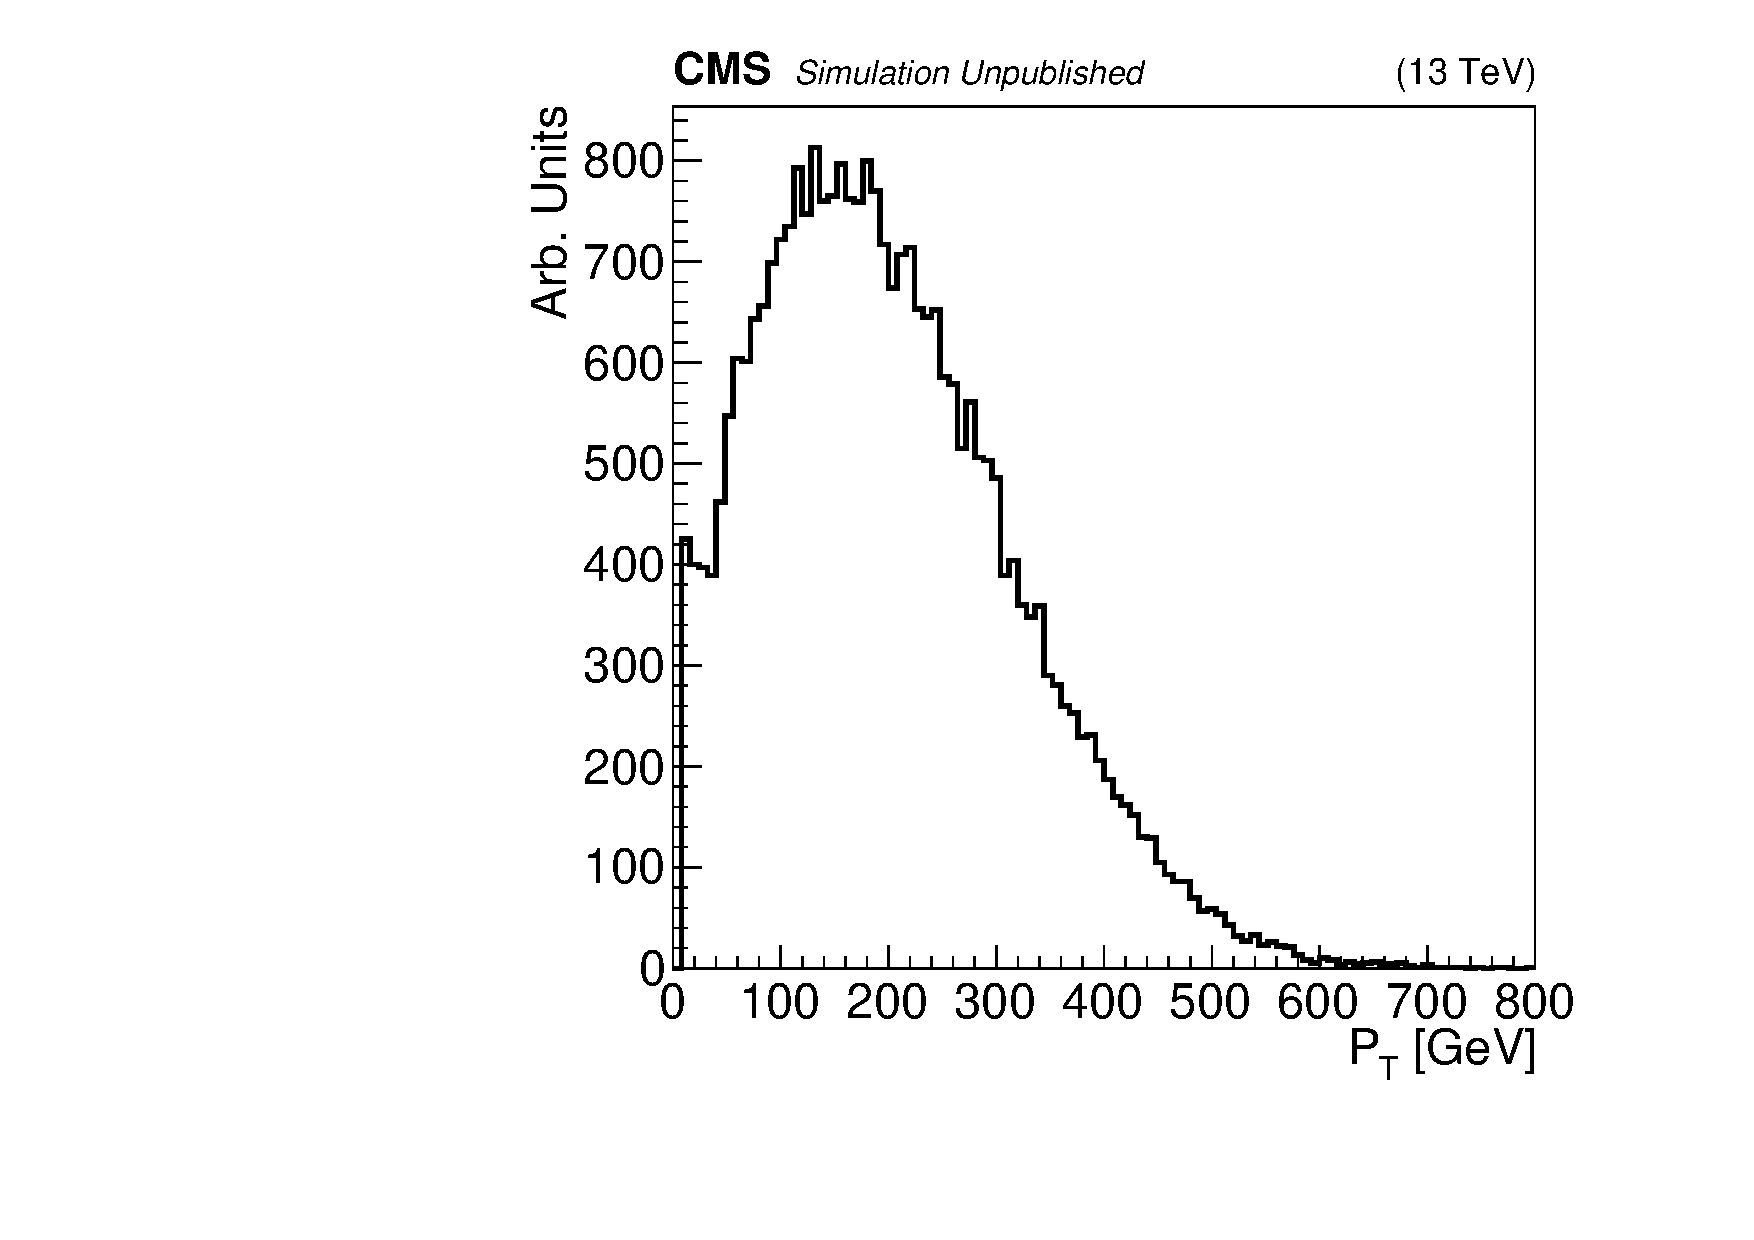
\includegraphics[width=2.4in]{figures/ptMatchedRecoJetTwo_mwr2200_mnu1100.pdf}
		\caption{jet from $\nul \rightarrow \ell jj$}\label{fig:wrLeptJetPtsd}
	\end{subfigure}
	\caption{The $\pt$ of leptons and jets reconstructed in $\WR \rightarrow \ell\ell jj$ events with $\mWR = 2.2$ $\TeV$ 
		and $\mnul = \frac{1}{2}\mWR$.}\label{fig:wrLeptJetPts}
\end{figure}

\begin{figure}
	\centering
	\begin{subfigure}[t]{2.4in}
		\centering
		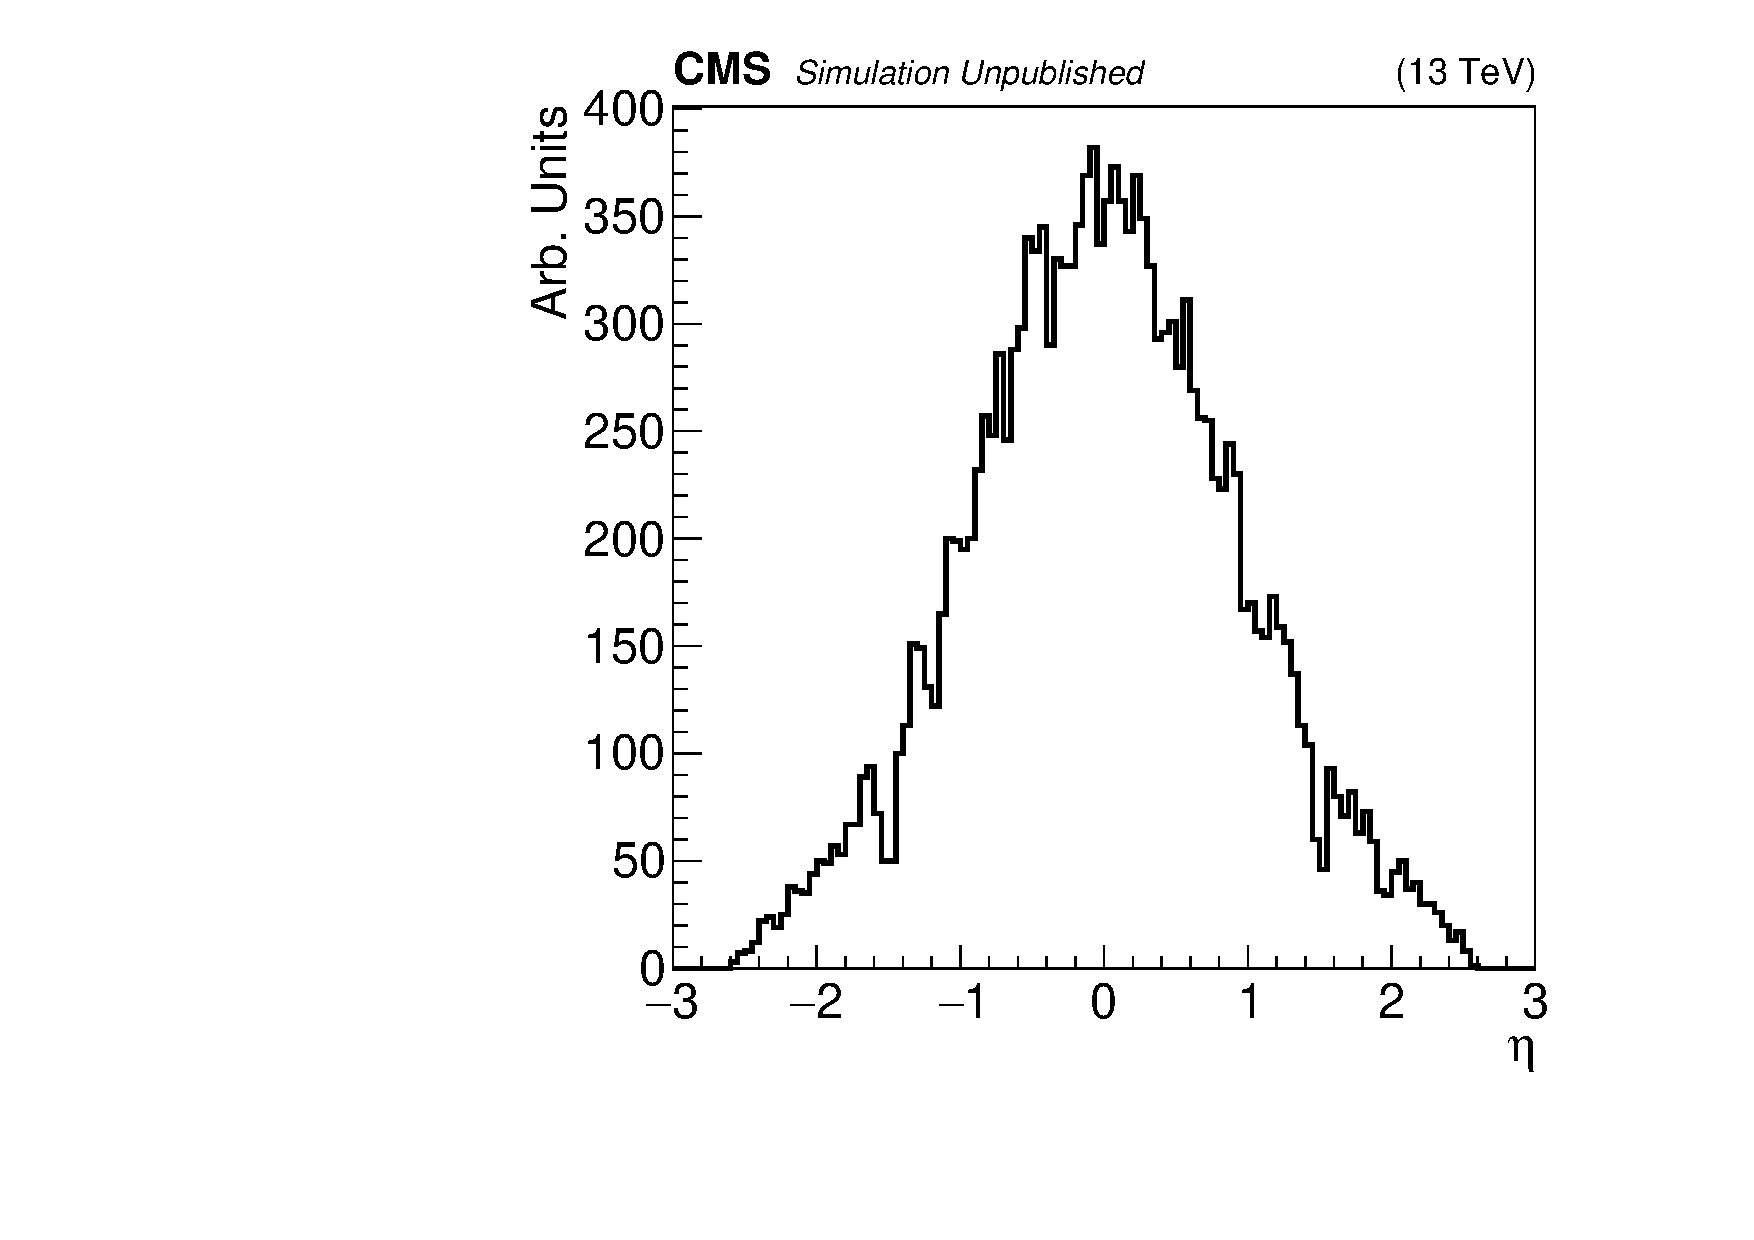
\includegraphics[width=2.4in]{figures/etaMatchedRecoEleFromWr_mwr2200_mnu1100.pdf}
		\caption{$\ell$ from $\WR \rightarrow \ell\nul$}\label{fig:wrLeptJetEtasa}
	\end{subfigure}
	\thickspace
	\begin{subfigure}[t]{2.4in}
		\centering
		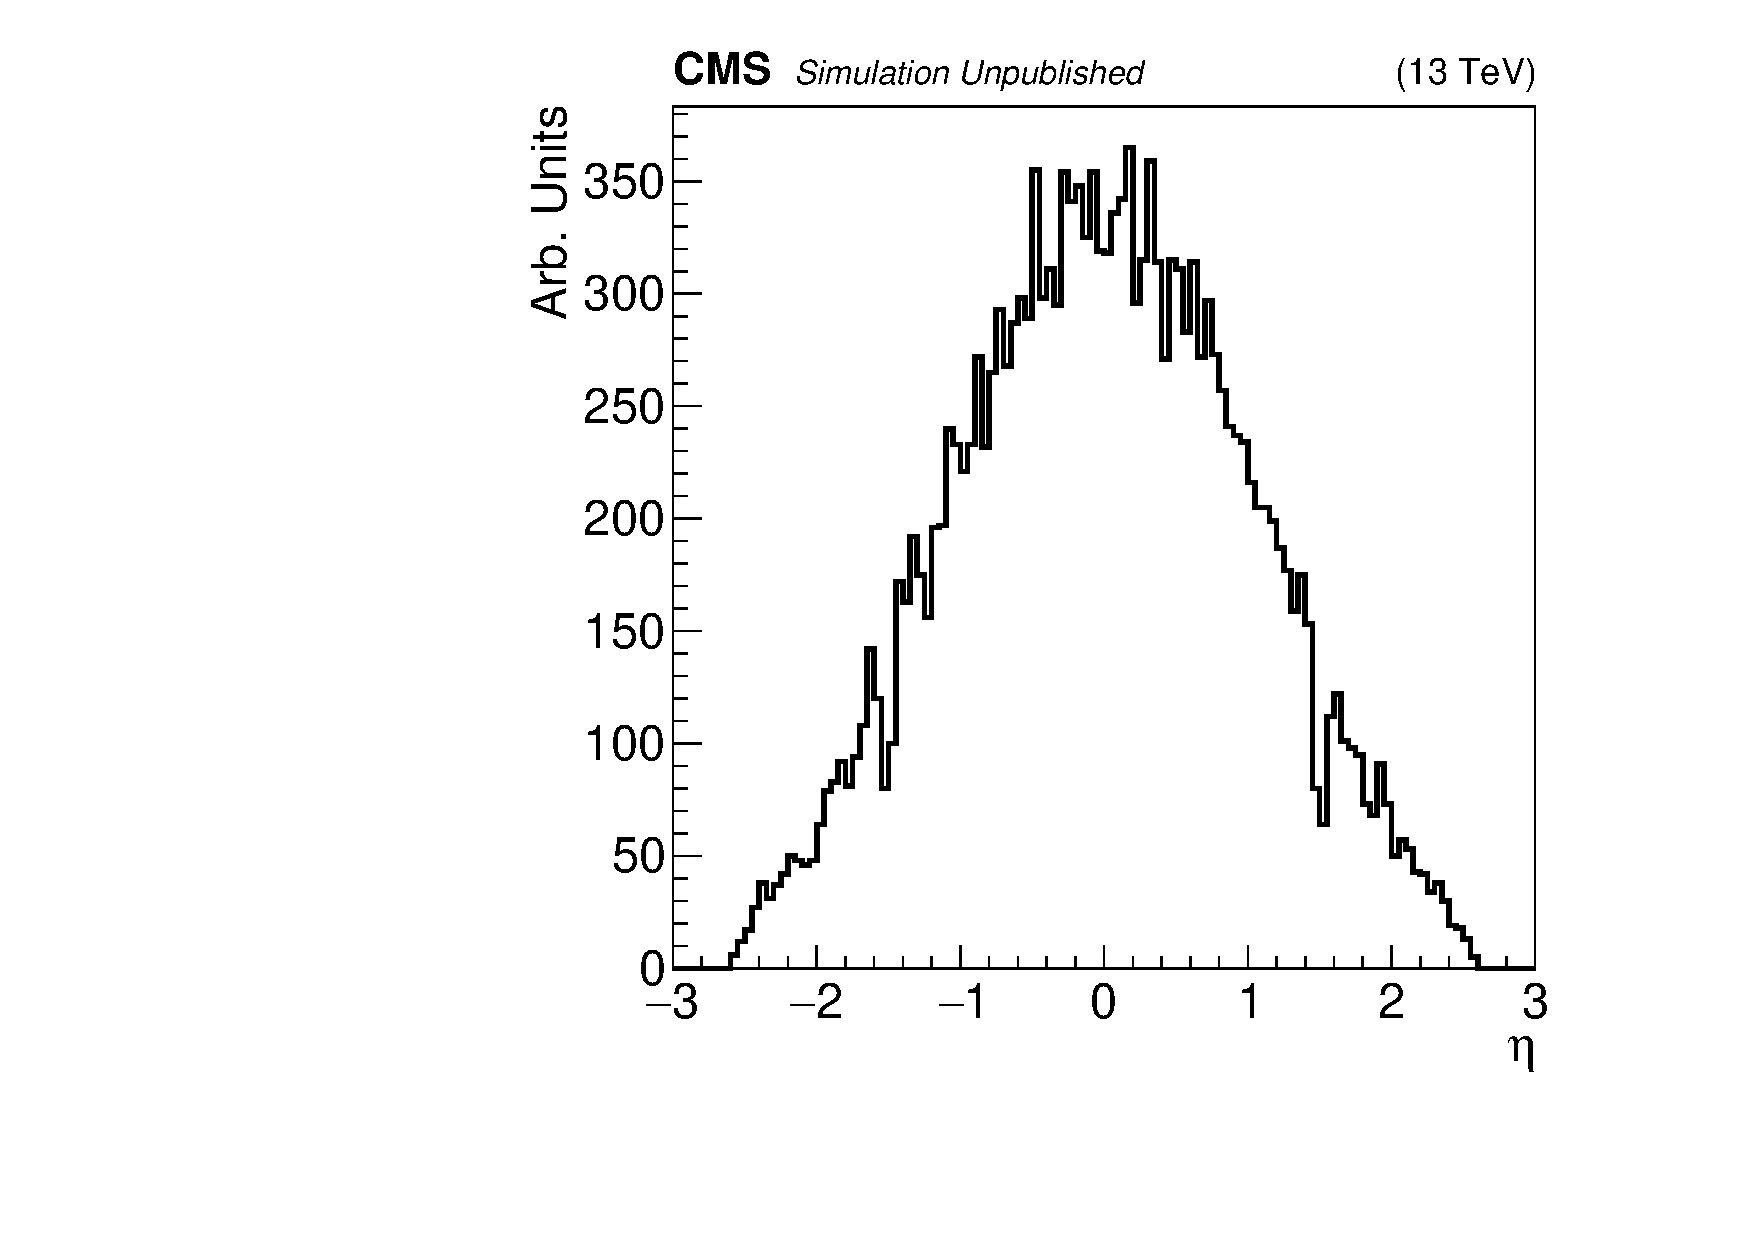
\includegraphics[width=2.4in]{figures/etaMatchedRecoEleFromNu_mwr2200_mnu1100.pdf}
		\caption{$\ell$ from $\nul \rightarrow \ell jj$}\label{fig:wrLeptJetEtasb}
	\end{subfigure}
	\newline
	\newline
	\newline
	\newline
	\begin{subfigure}[t]{2.4in}
		\centering
		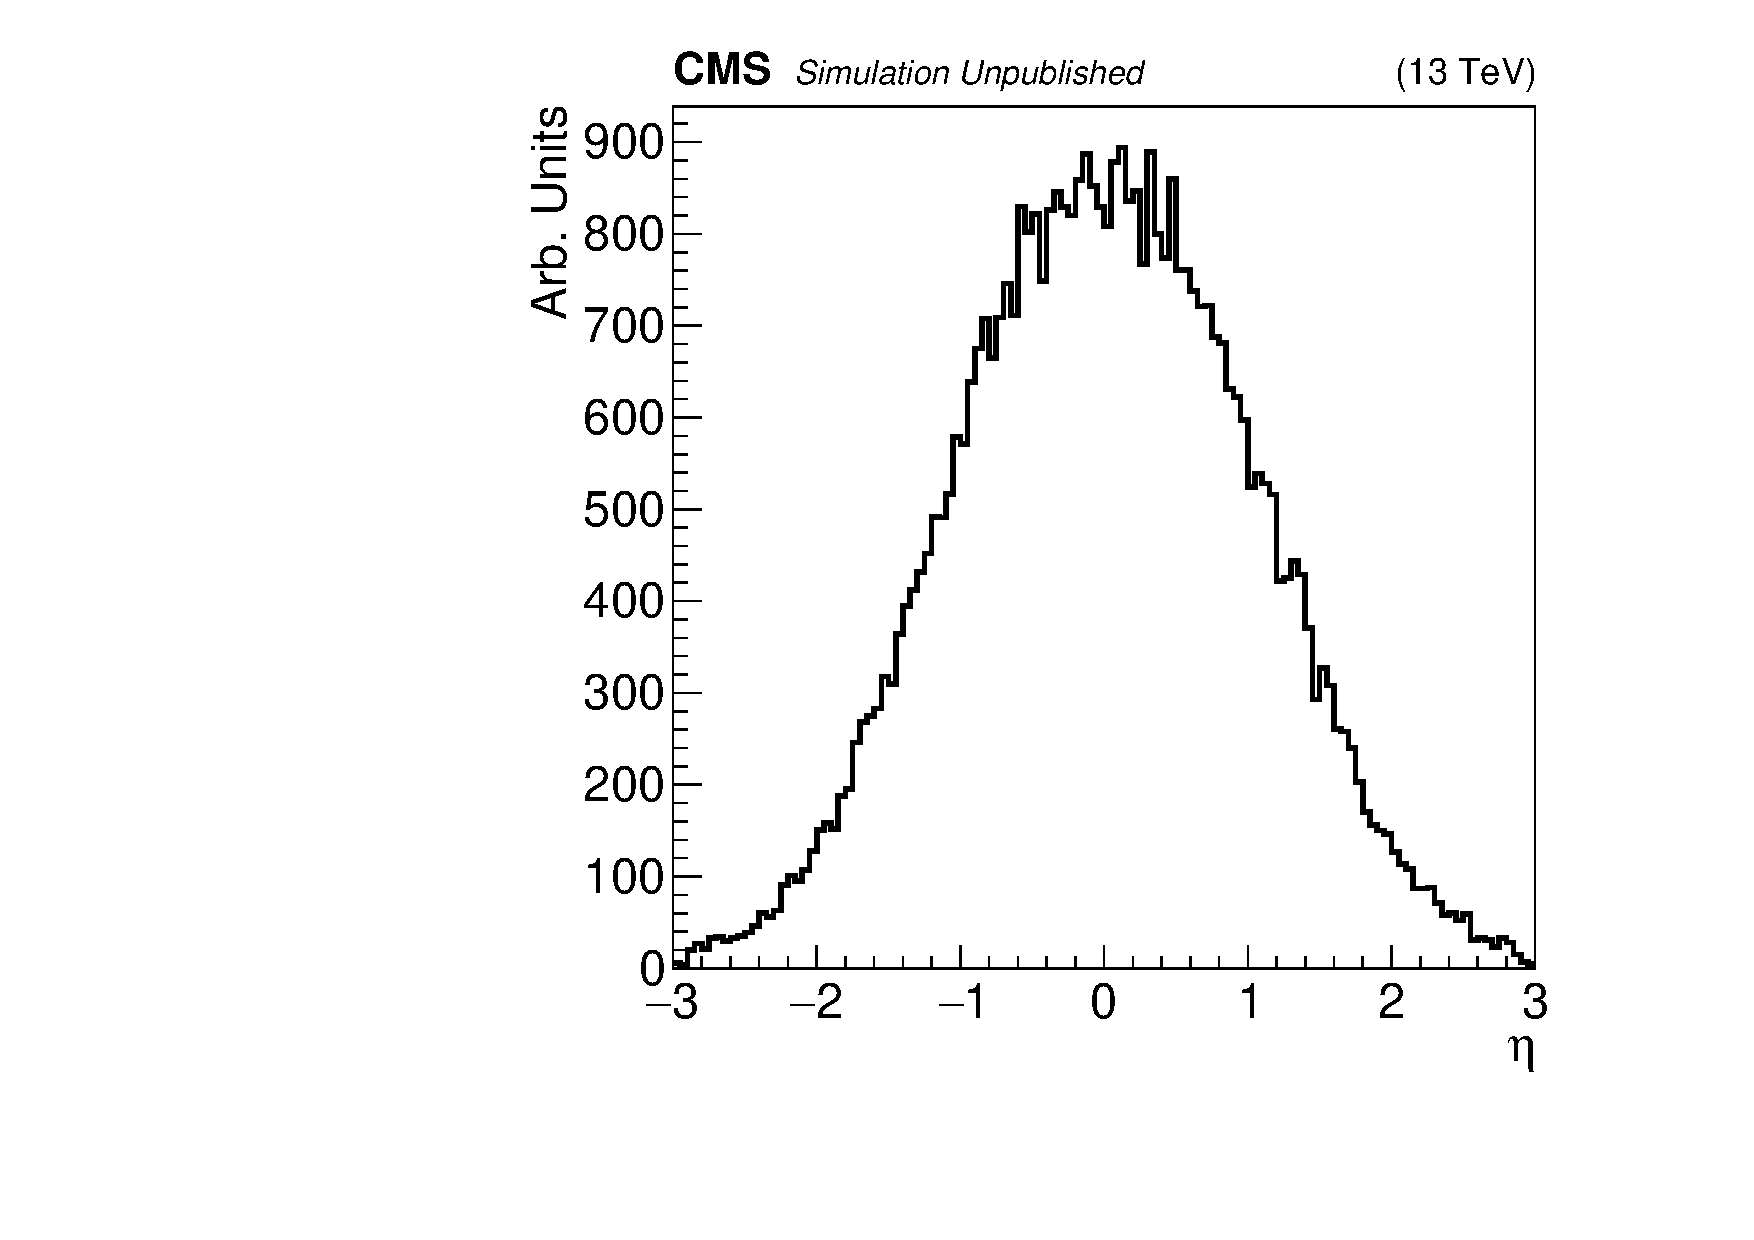
\includegraphics[width=2.4in]{figures/etaMatchedRecoJetOne_mwr2200_mnu1100.pdf}
		\caption{jet from $\nul \rightarrow \ell jj$}\label{fig:wrLeptJetEtasc}
	\end{subfigure}
	\thickspace
	\begin{subfigure}[t]{2.4in}
		\centering
		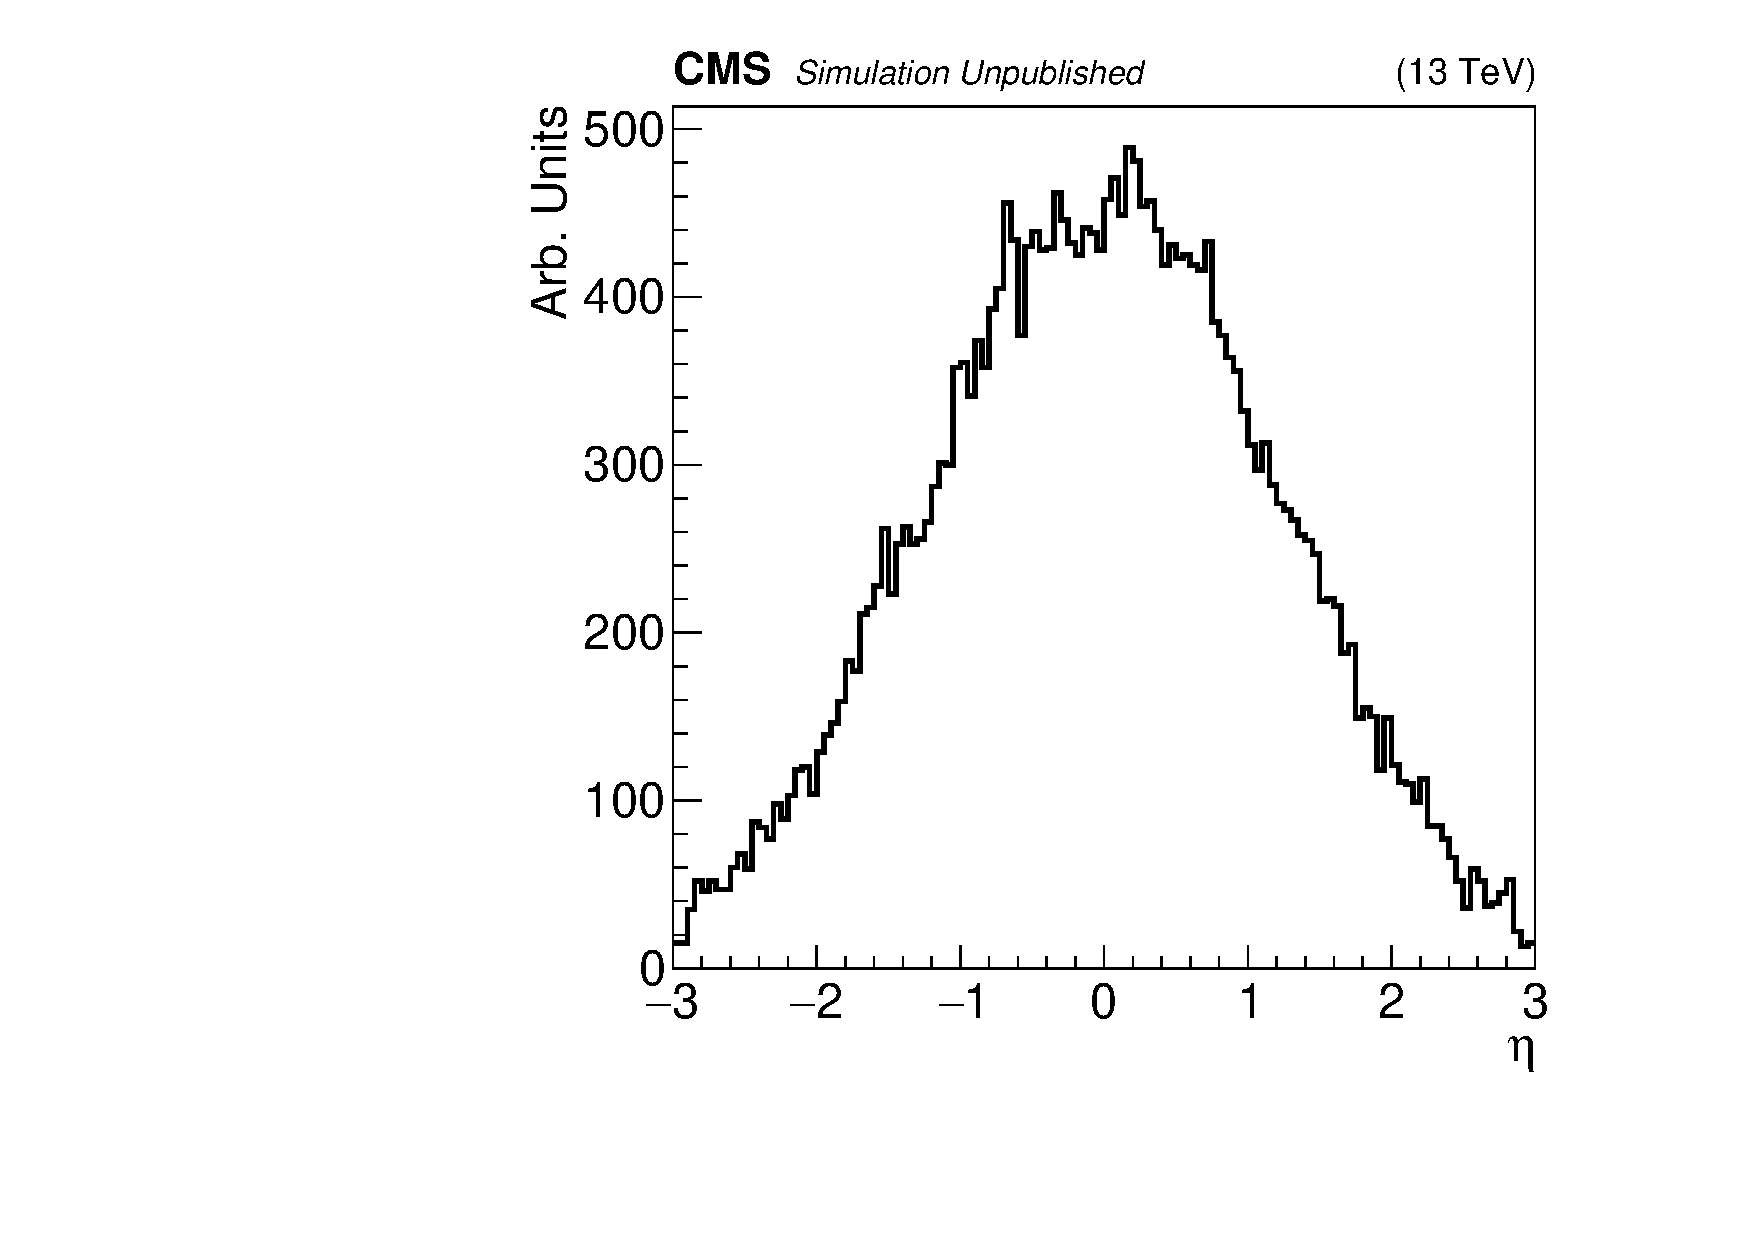
\includegraphics[width=2.4in]{figures/etaMatchedRecoJetTwo_mwr2200_mnu1100.pdf}
		\caption{jet from $\nul \rightarrow \ell jj$}\label{fig:wrLeptJetEtasd}
	\end{subfigure}
	\caption{The $\eta$ of leptons and jets reconstructed in $\WR \rightarrow \ell\ell jj$ events with $\mWR = 2.2$ $\TeV$ 
		and $\mnul = \frac{1}{2}\mWR$.}\label{fig:wrLeptJetEtas}
\end{figure}

\begin{figure}
	\centering
	\begin{subfigure}[t]{2.4in}
		\centering
		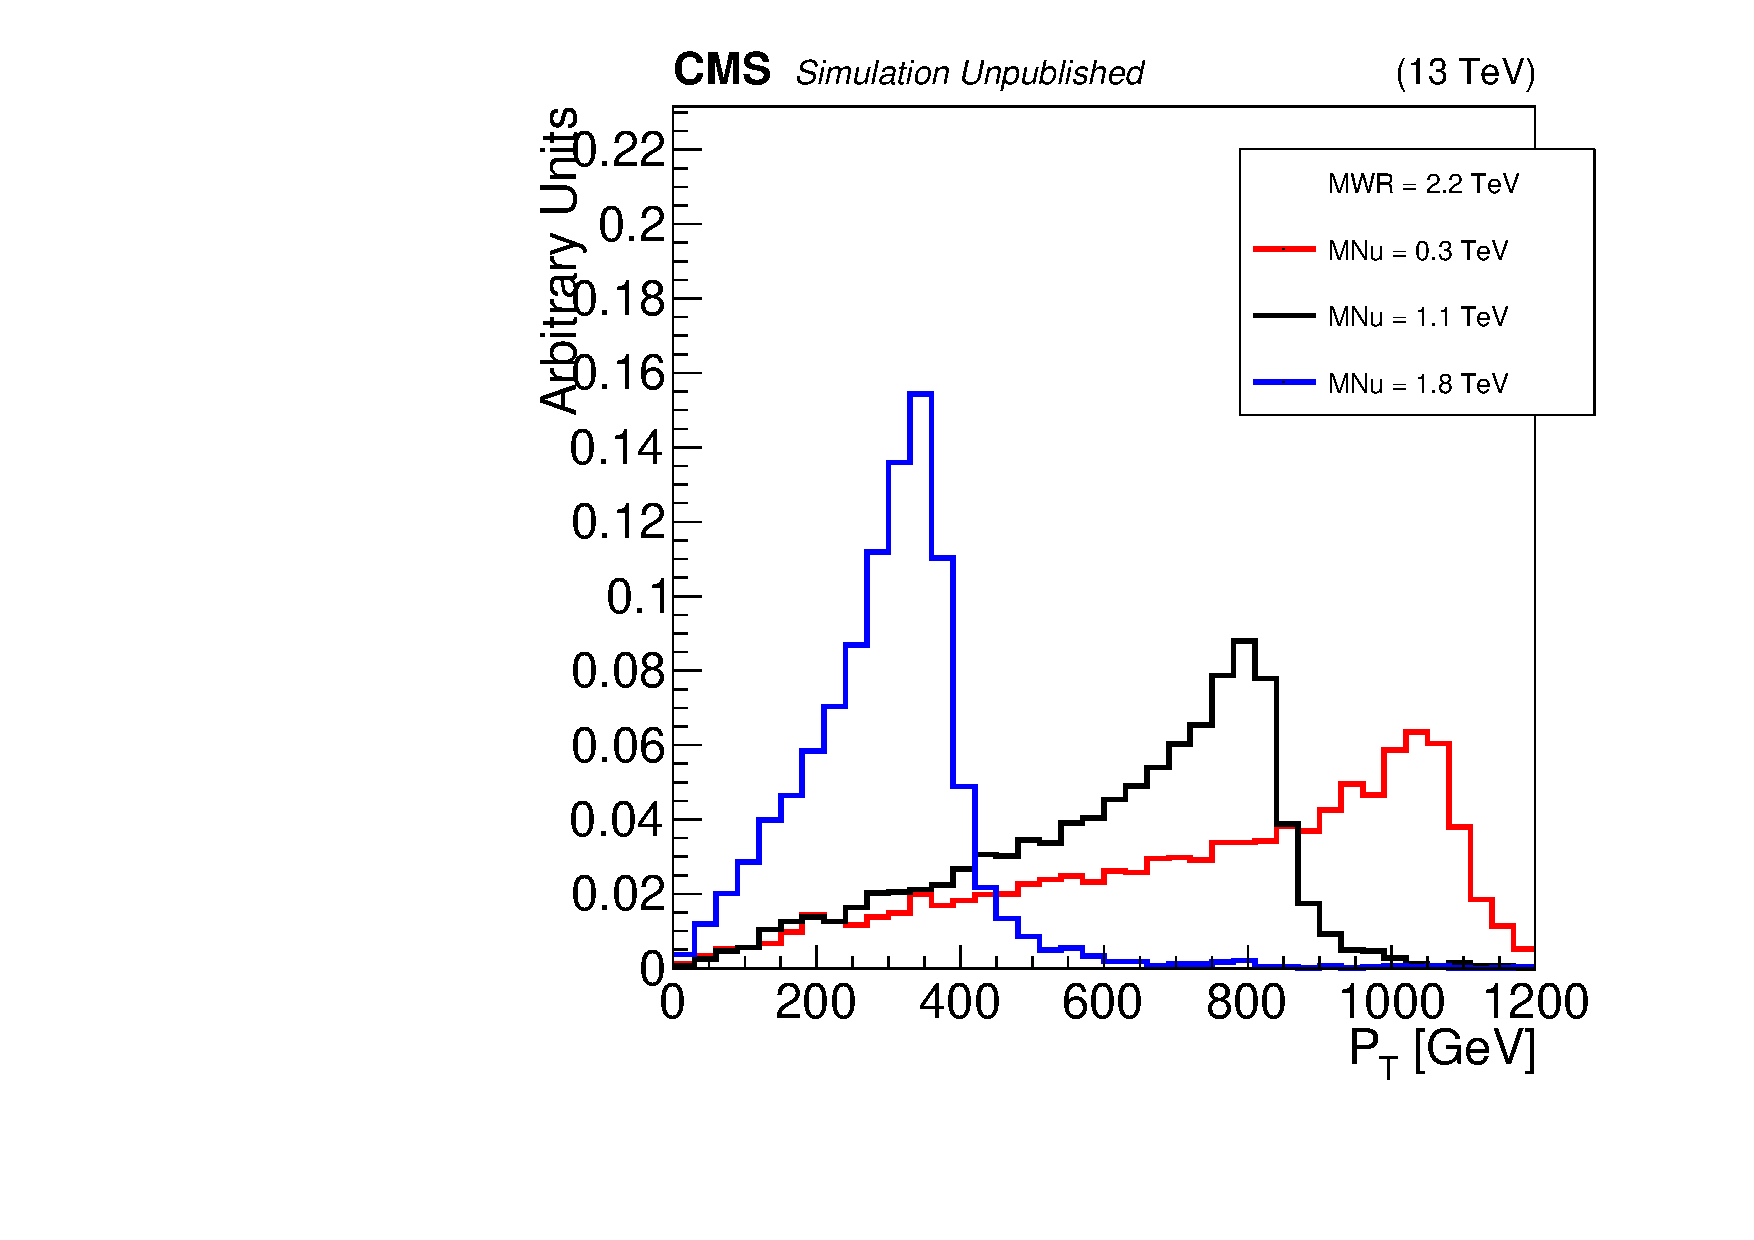
\includegraphics[width=2.4in]{figures/ptGenLeptFromFstHvyPtcl_MWR_2200_several_MNu_private.pdf}
		\caption{$\ell$ from $\WR \rightarrow \ell\nul$}\label{fig:wrLeptQrkPtsVarMNua}
	\end{subfigure}
	\thickspace
	\begin{subfigure}[t]{2.4in}
		\centering
		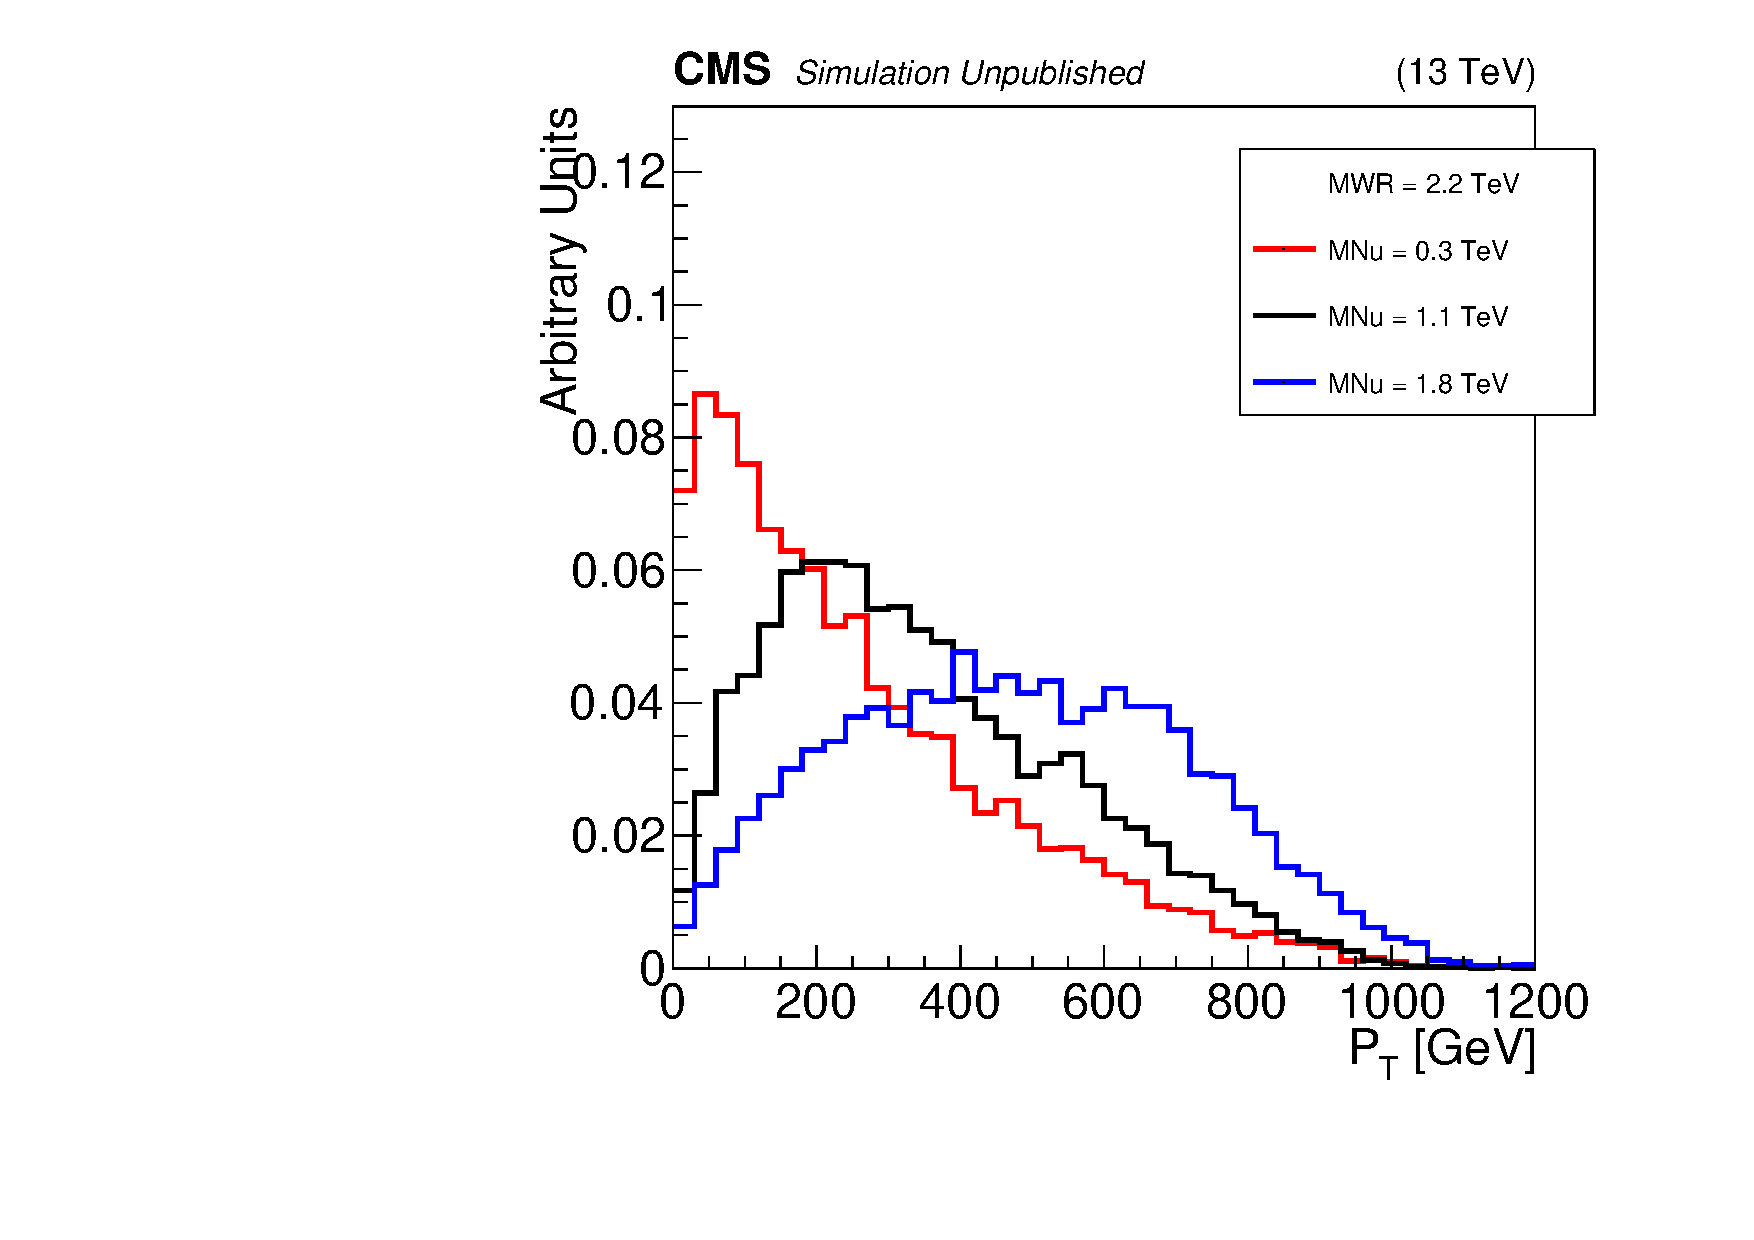
\includegraphics[width=2.4in]{figures/ptGenLeptFromScdHvyPtcl_MWR_2200_several_MNu_private.pdf}
		\caption{$\ell$ from $\nul \rightarrow \ell qq$}\label{fig:wrLeptQrkPtsVarMNub}
	\end{subfigure}
	\newline
	\newline
	\newline
	\newline
	\begin{subfigure}[t]{2.4in}
		\centering
		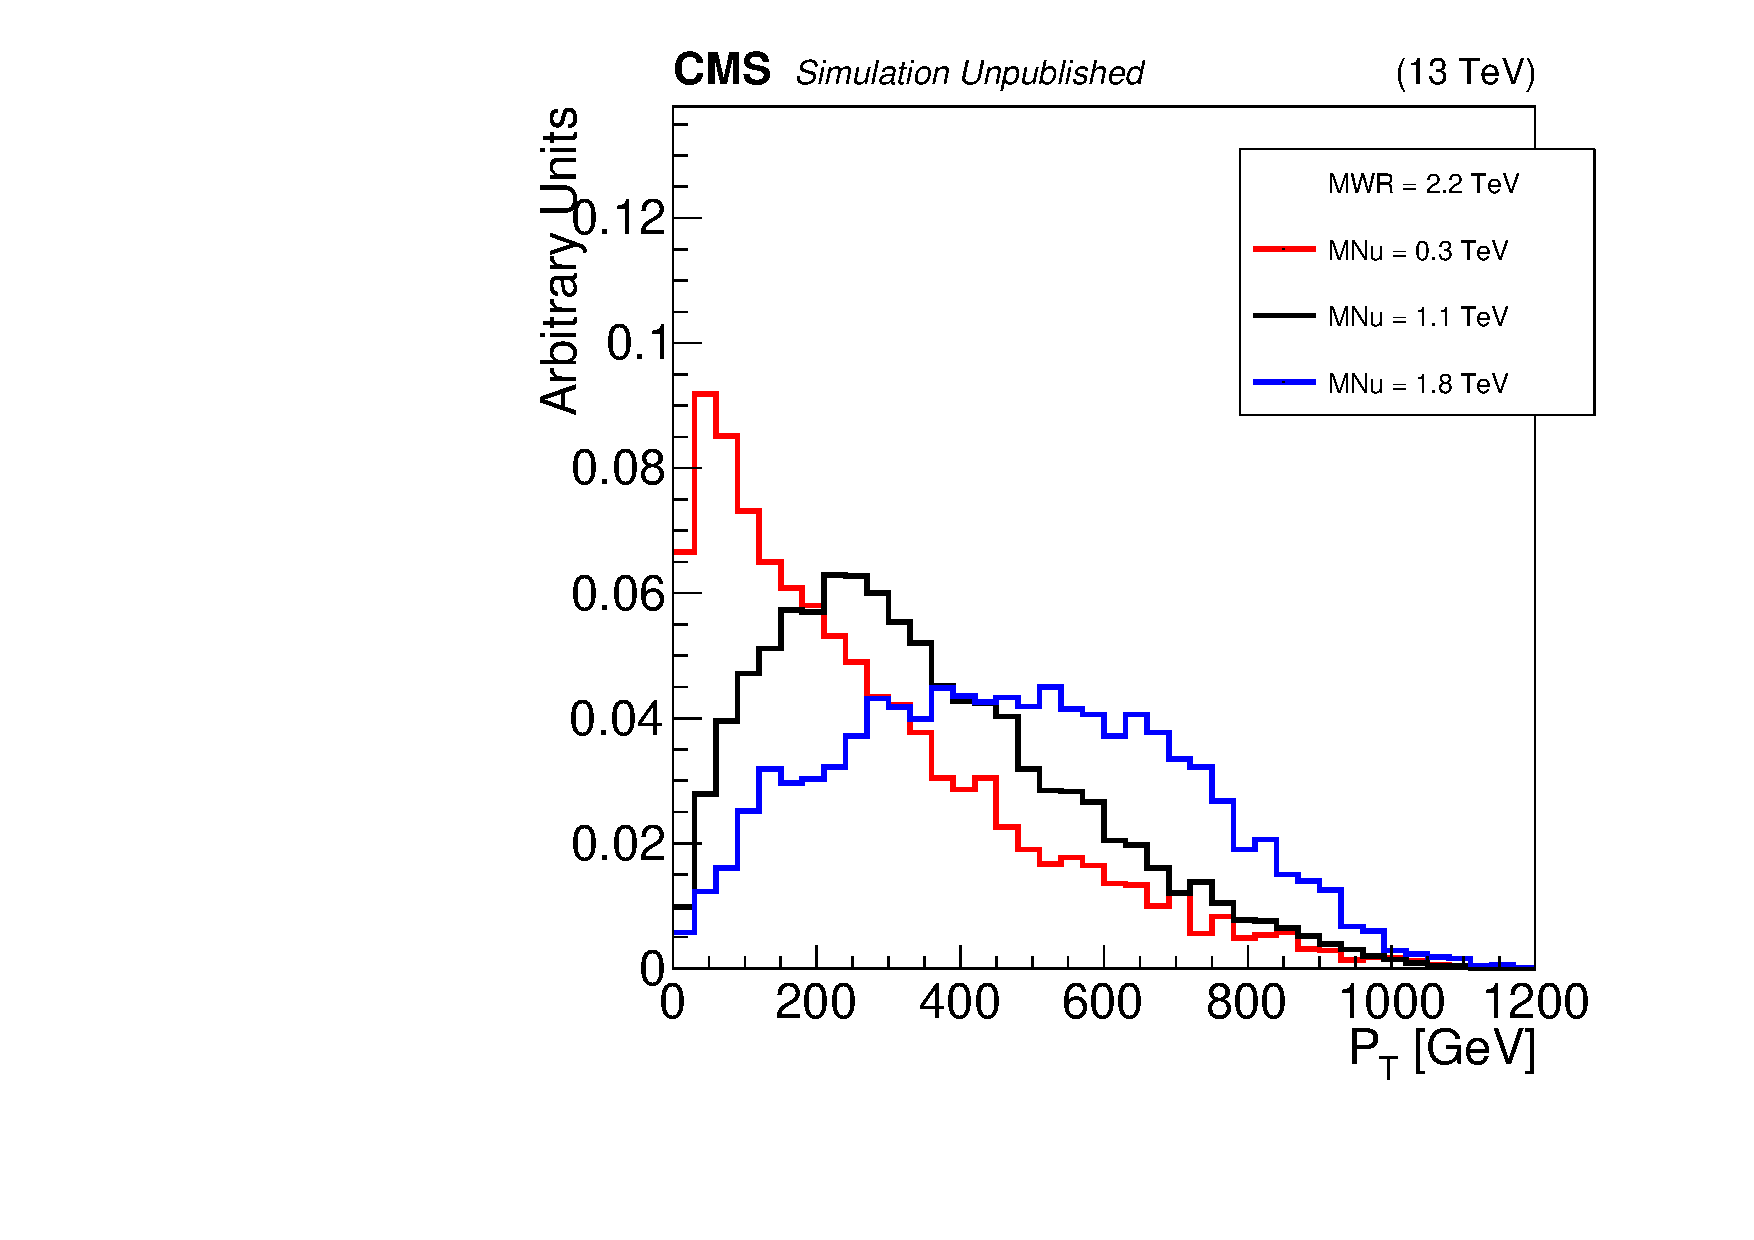
\includegraphics[width=2.4in]{figures/ptGenQuarkOneFromScdHvyPtcl_MWR_2200_several_MNu_private.pdf}
		\caption{quark from $\nul \rightarrow \ell qq$}\label{fig:wrLeptQrkPtsVarMNuc}
	\end{subfigure}
	\thickspace
	\begin{subfigure}[t]{2.4in}
		\centering
		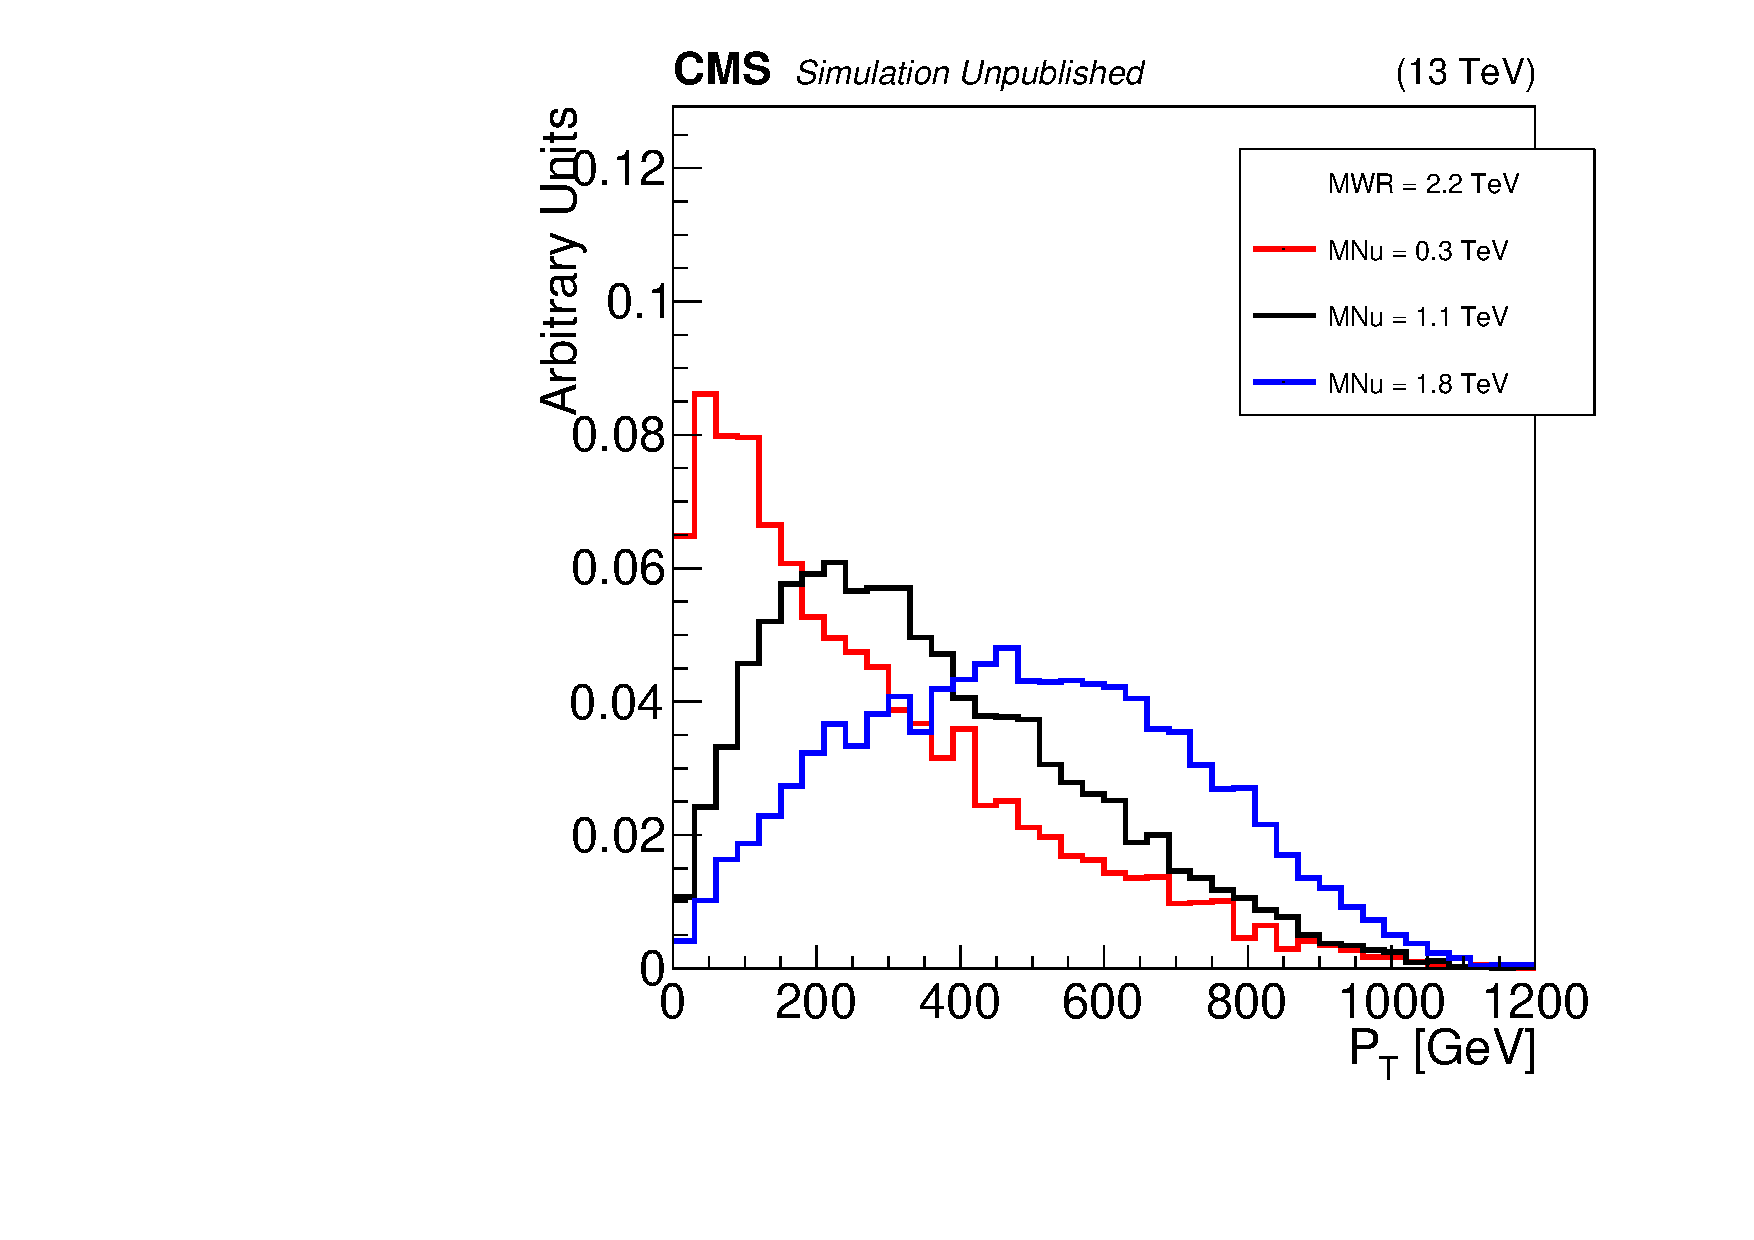
\includegraphics[width=2.4in]{figures/ptGenQuarkTwoFromScdHvyPtcl_MWR_2200_several_MNu_private.pdf}
		\caption{quark from $\nul \rightarrow \ell qq$}\label{fig:wrLeptQrkPtsVarMNud}
	\end{subfigure}
	\caption{The $\pt$ of leptons and quarks produced in $\WR \rightarrow \ell\ell qq$ events with $\mWR = 2.2$ $\TeV$ 
		and different \mnul.}\label{fig:wrLeptQrkPtsVarMNu}
\end{figure}

\begin{figure}[h]
	\centering
	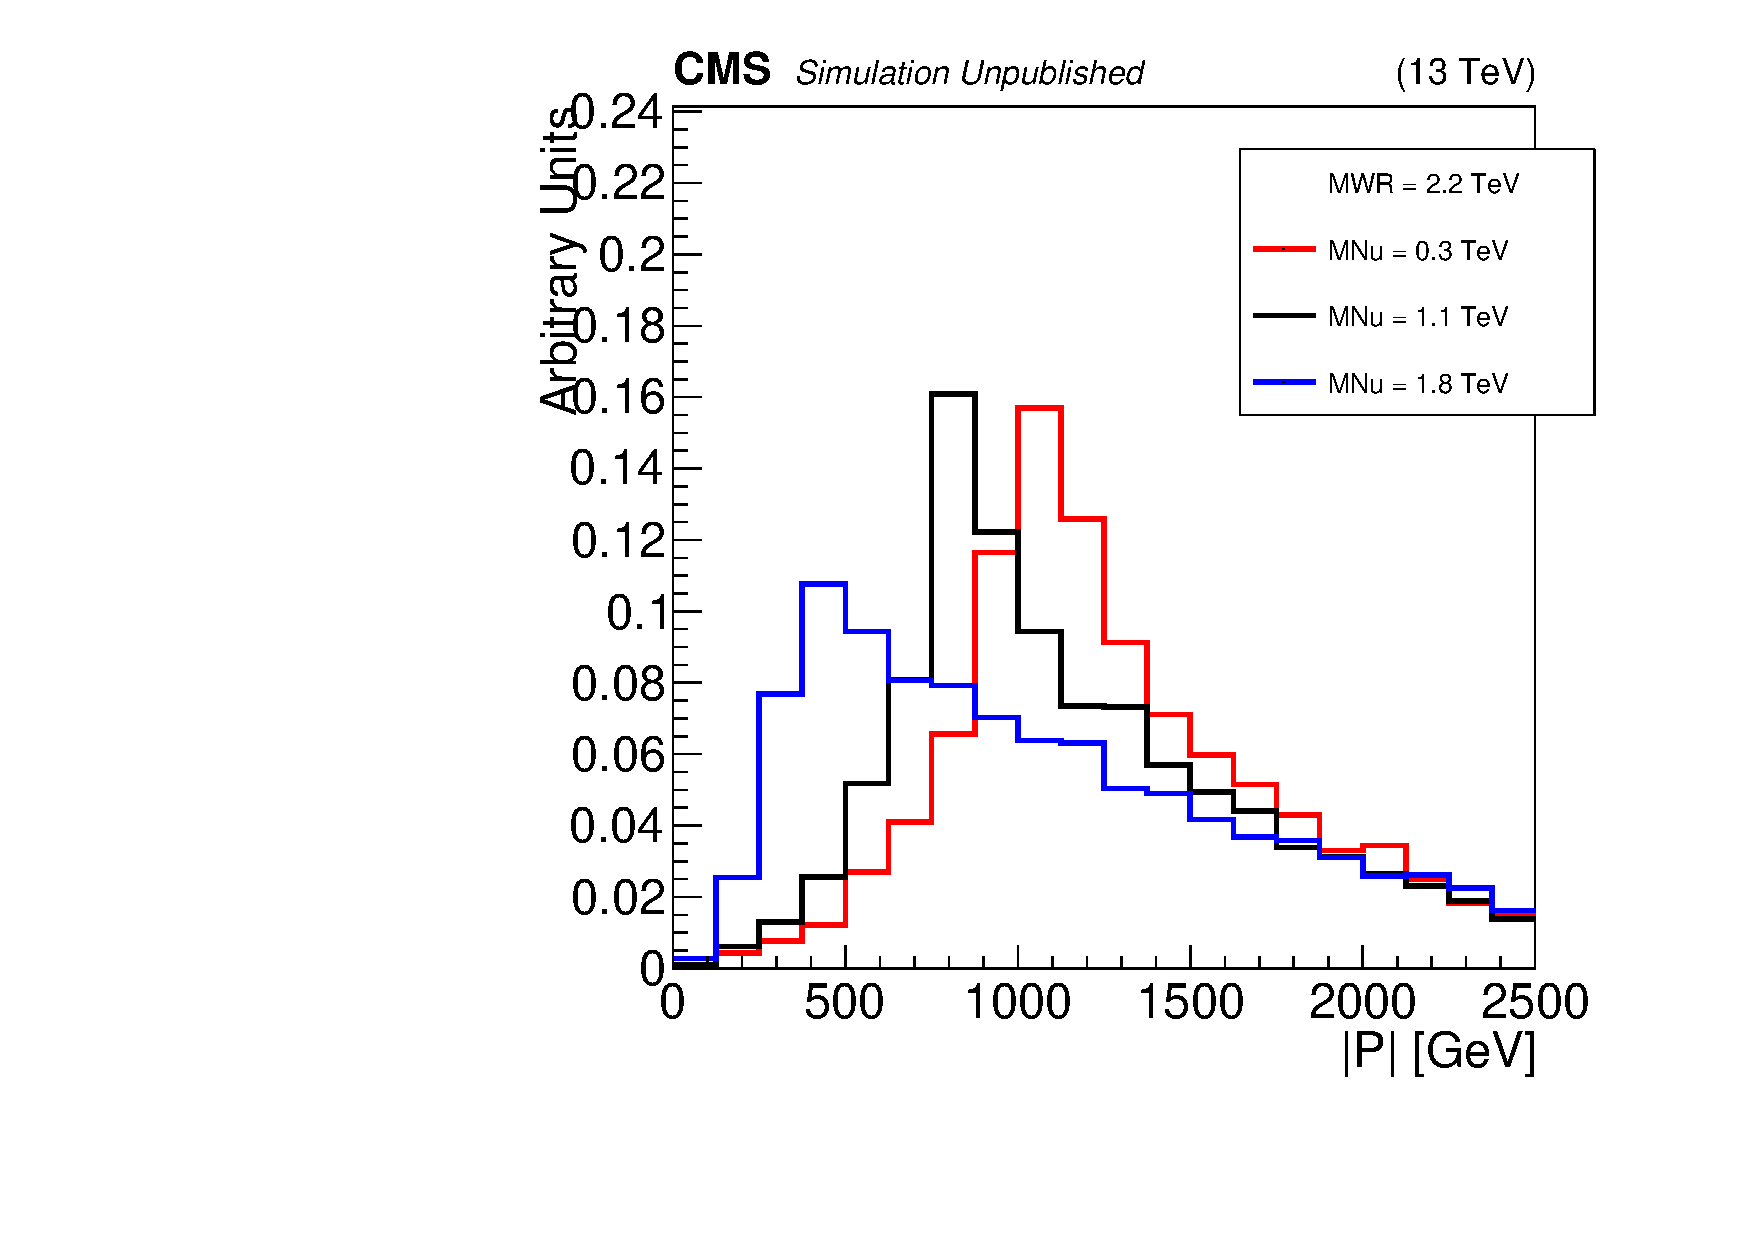
\includegraphics[width=0.5\textwidth]{figures/genNuMomMag_MWR_2200_several_MNu_private.pdf}
	\caption{The $|p|$ of the \nul produced in $\WR \rightarrow \ell\nul$ events with $\mWR = 2.2$ $\TeV$ and different \mnul.}
	\label{fig:hvyNuMomentumVarMNu}
\end{figure}

\begin{figure}
	\centering
	\begin{subfigure}[t]{2.4in}
		\centering
		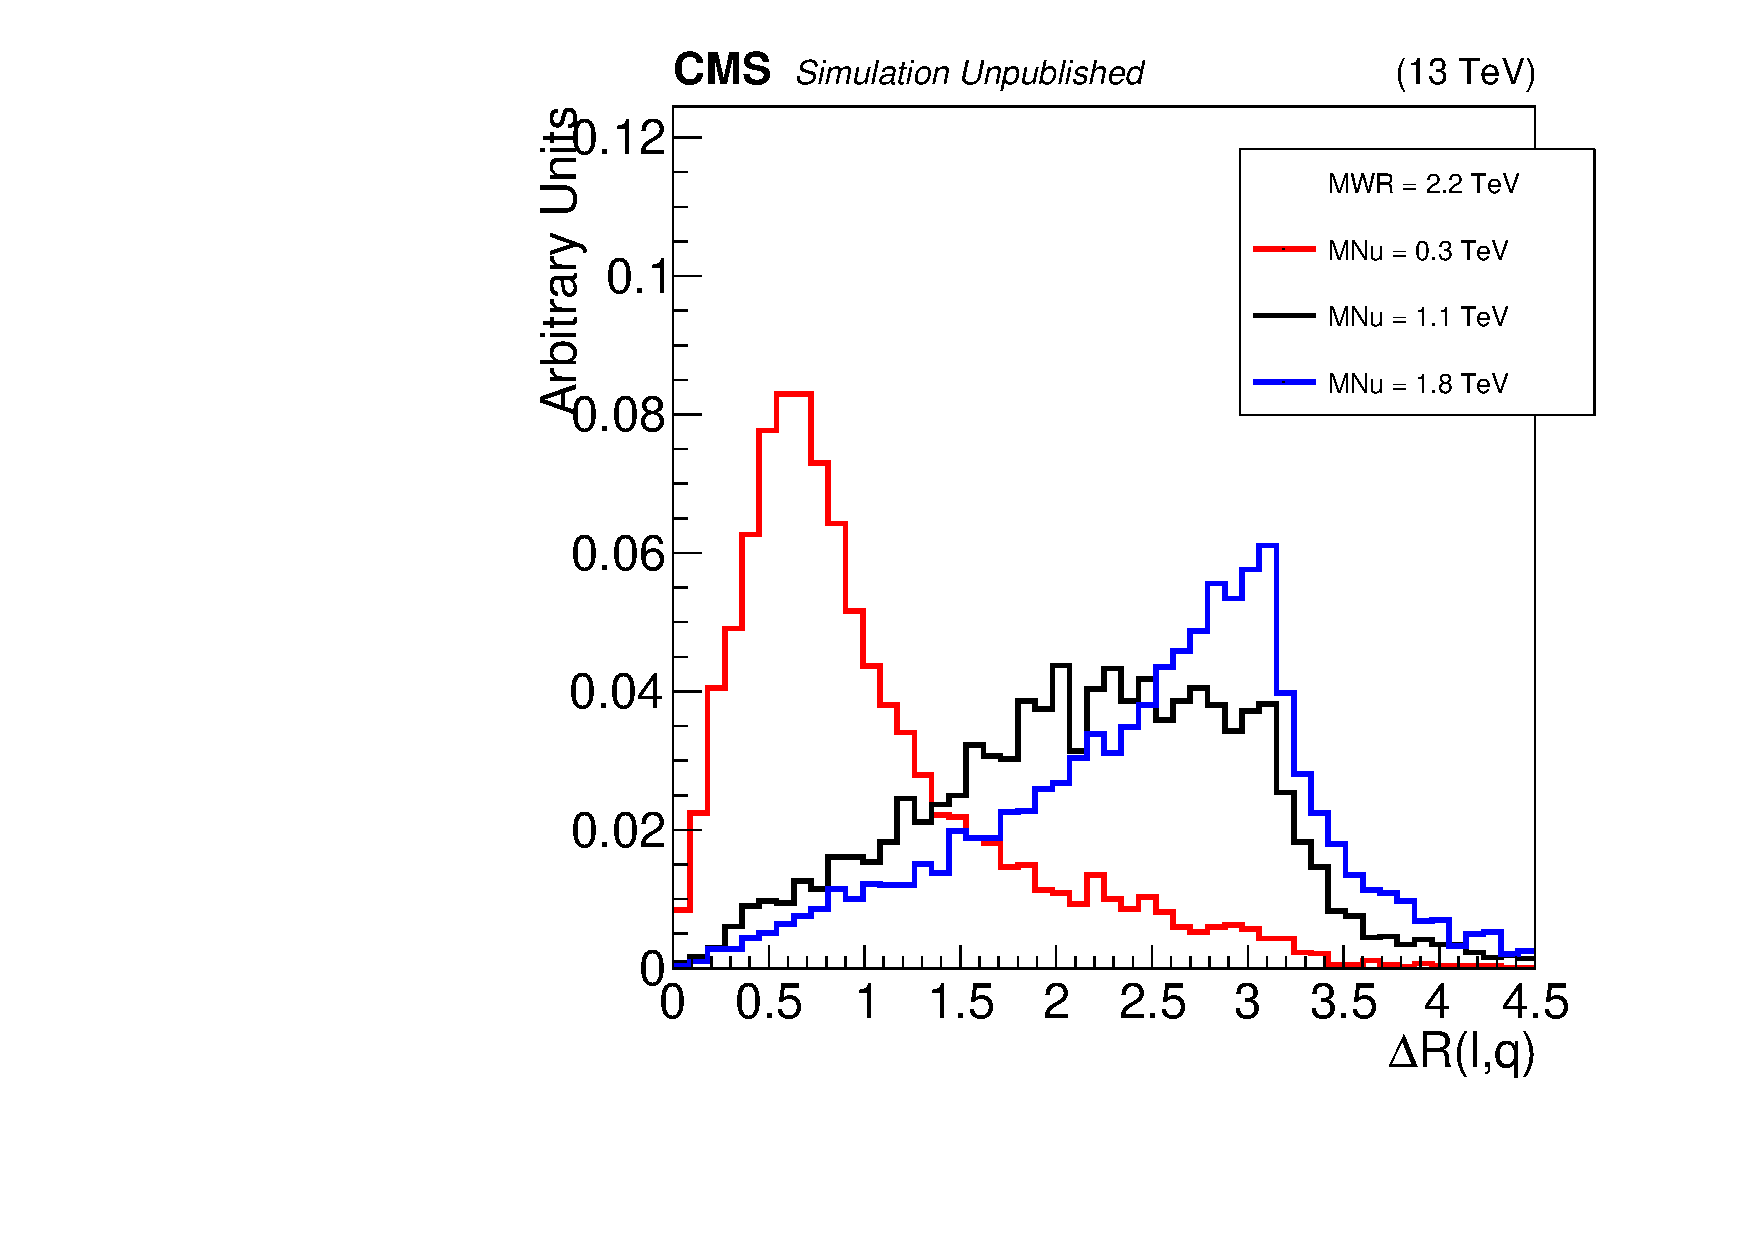
\includegraphics[width=2.4in]{figures/dRgenLeptonFromScdHvyPtclGenQuarkOneFromScdHvyPtcl_MWR_2200_several_MNu_private.pdf}
		%\caption{ }\label{fig:wrDrLeptQrkVarMNua}
	\end{subfigure}
	\thickspace
	\begin{subfigure}[t]{2.4in}
		\centering
		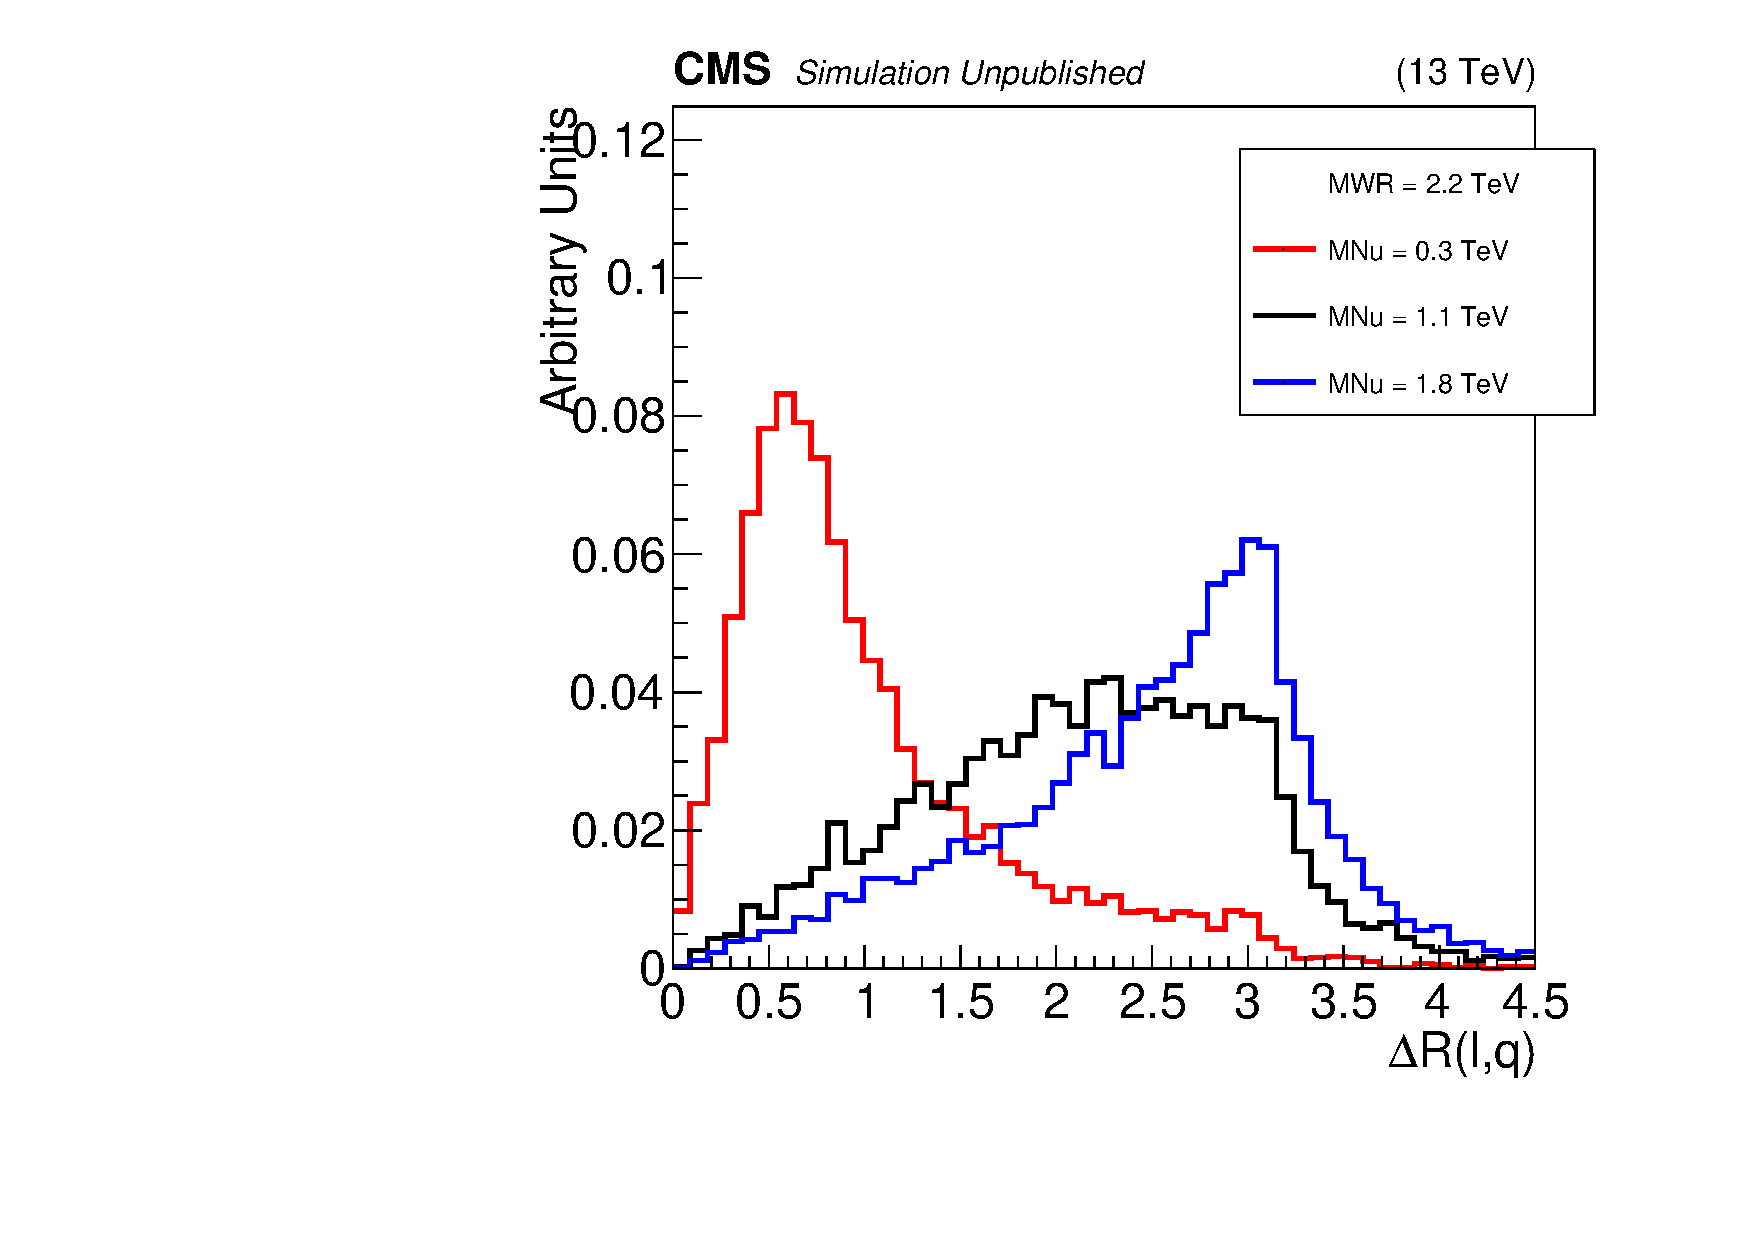
\includegraphics[width=2.4in]{figures/dRgenLeptonFromScdHvyPtclGenQuarkTwoFromScdHvyPtcl_MWR_2200_several_MNu_private.pdf}
		%\caption{ }\label{fig:wrDrLeptQrkVarMNub}
	\end{subfigure}
	\caption{The $\Delta R(\ell,q)$ separation between the $\ell$ and both quarks produced in $\nul \rightarrow \ell qq$ 
		in $\WR \rightarrow \ell\ell qq$ events with $\mWR = 2.2$ $\TeV$ and different \mnul.}\label{fig:wrDrLeptQrkVarMNu}
\end{figure}

\begin{figure}[h]
	\centering
	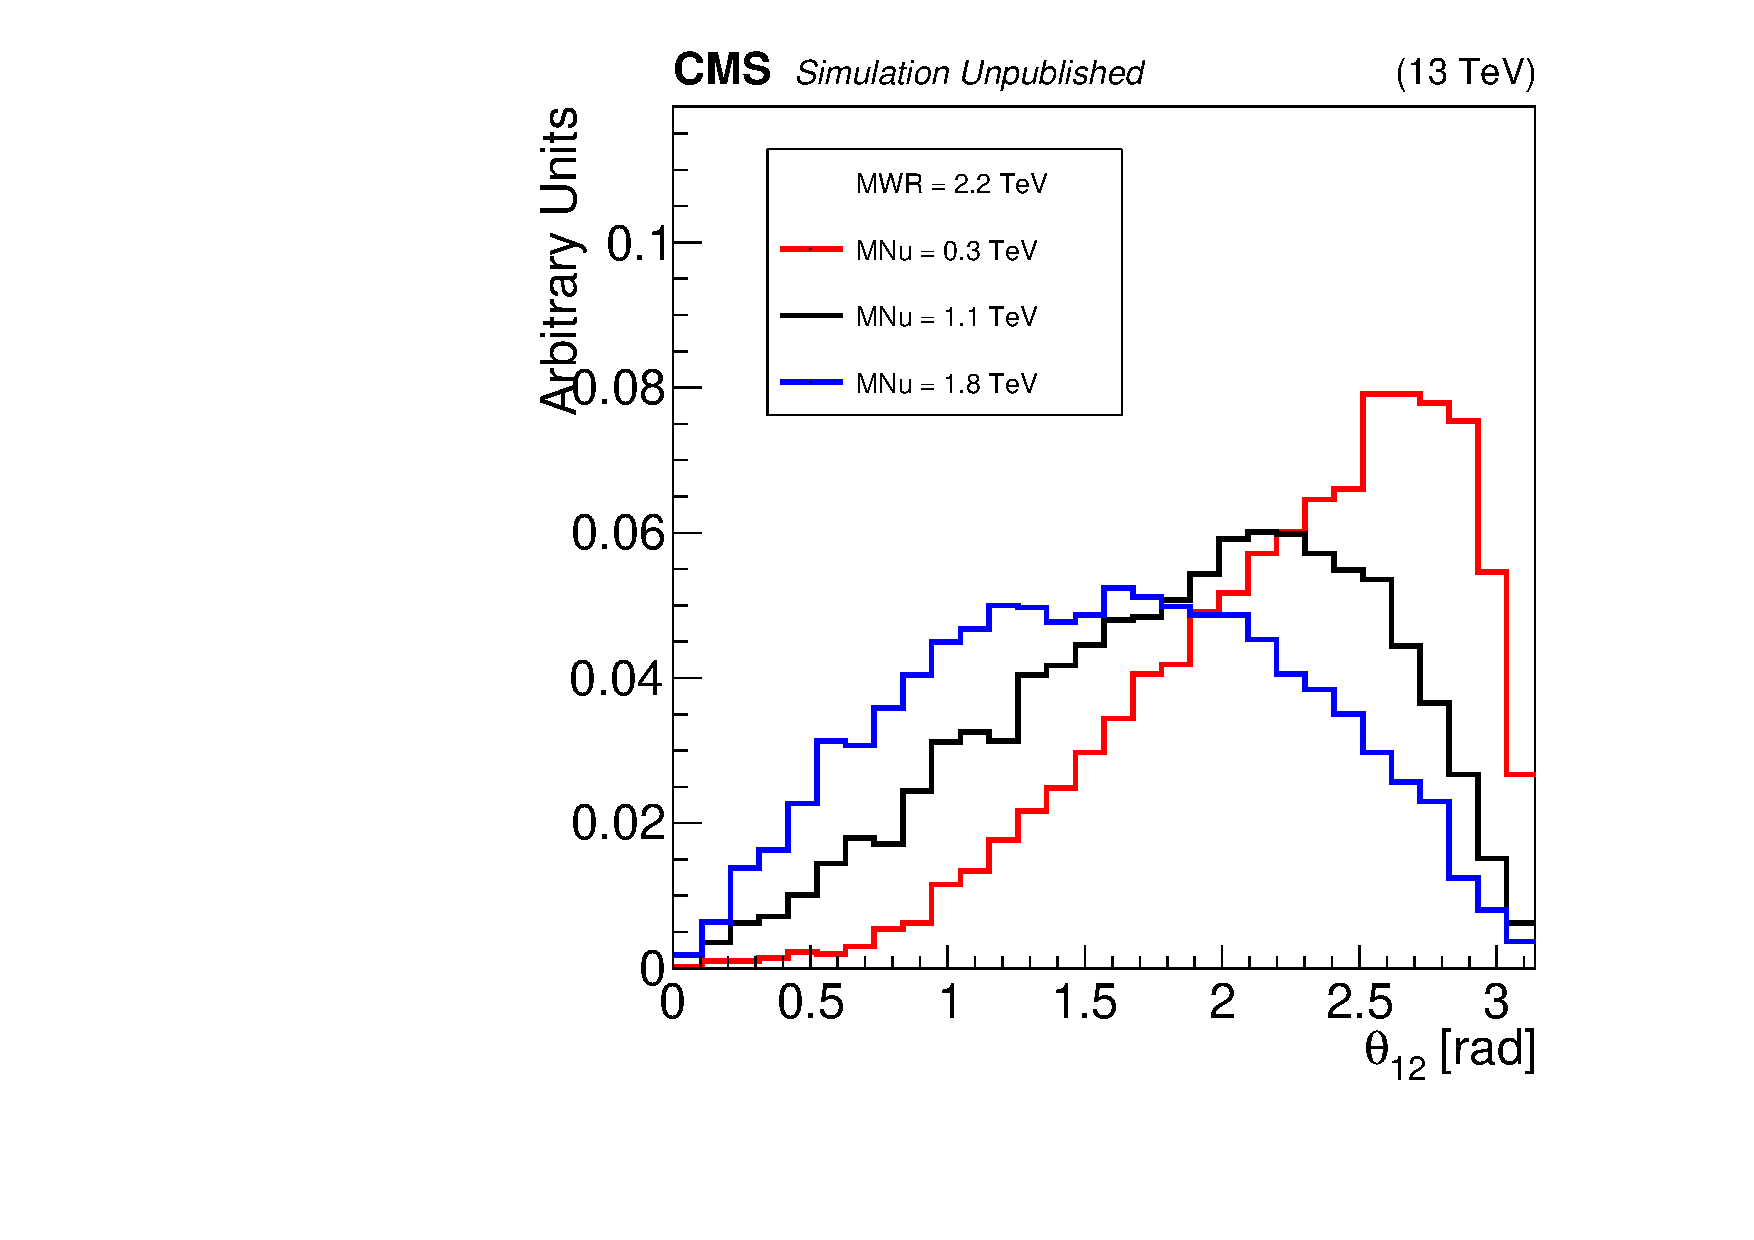
\includegraphics[width=0.5\textwidth]{figures/angleBtwnGenLepts_MWR_2200_several_MNu_private.pdf}
	\caption{The angle $\theta_{12}$ between the two leptons produced in $\WR \rightarrow \ell_{1}\ell_{2} qq$ events with 
		$\mWR = 2.2$ $\TeV$ and different \mnul.}
	\label{fig:wrLeptAngleSepVarMNu}
\end{figure}

\begin{figure}[h]
	\centering
	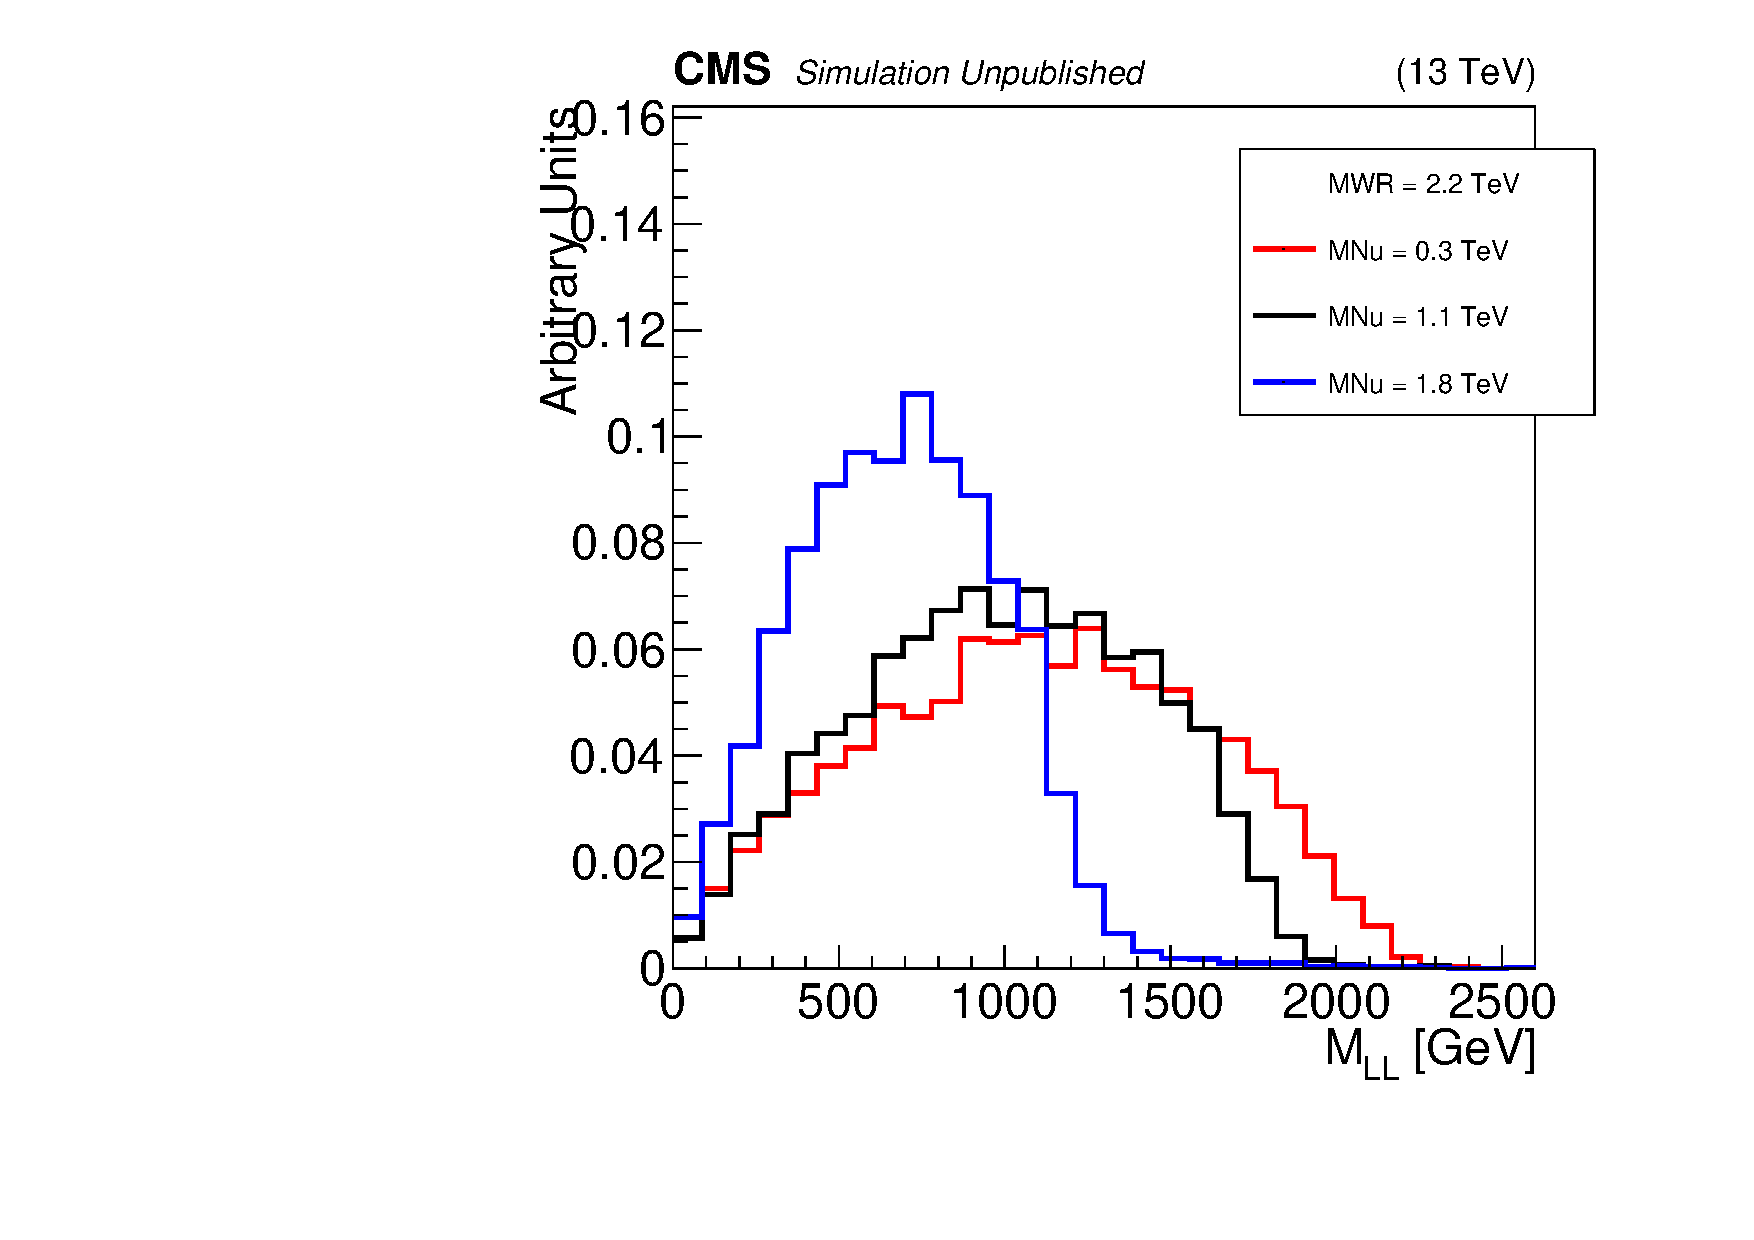
\includegraphics[width=0.5\textwidth]{figures/dileptonMassFromGenLeptonsFromFstAndScdHvyPtcl_MWR_2200_several_MNu_private.pdf}
	\caption{The $\Mll$ of the two leptons produced in $\WR \rightarrow \ell\ell qq$ events with $\mWR = 2.2$ $\TeV$ and 
	different \mnul.}
	\label{fig:wrMllVarMNu}
\end{figure}

\begin{figure}
	\centering
	\begin{subfigure}[t]{2.4in}
		\centering
		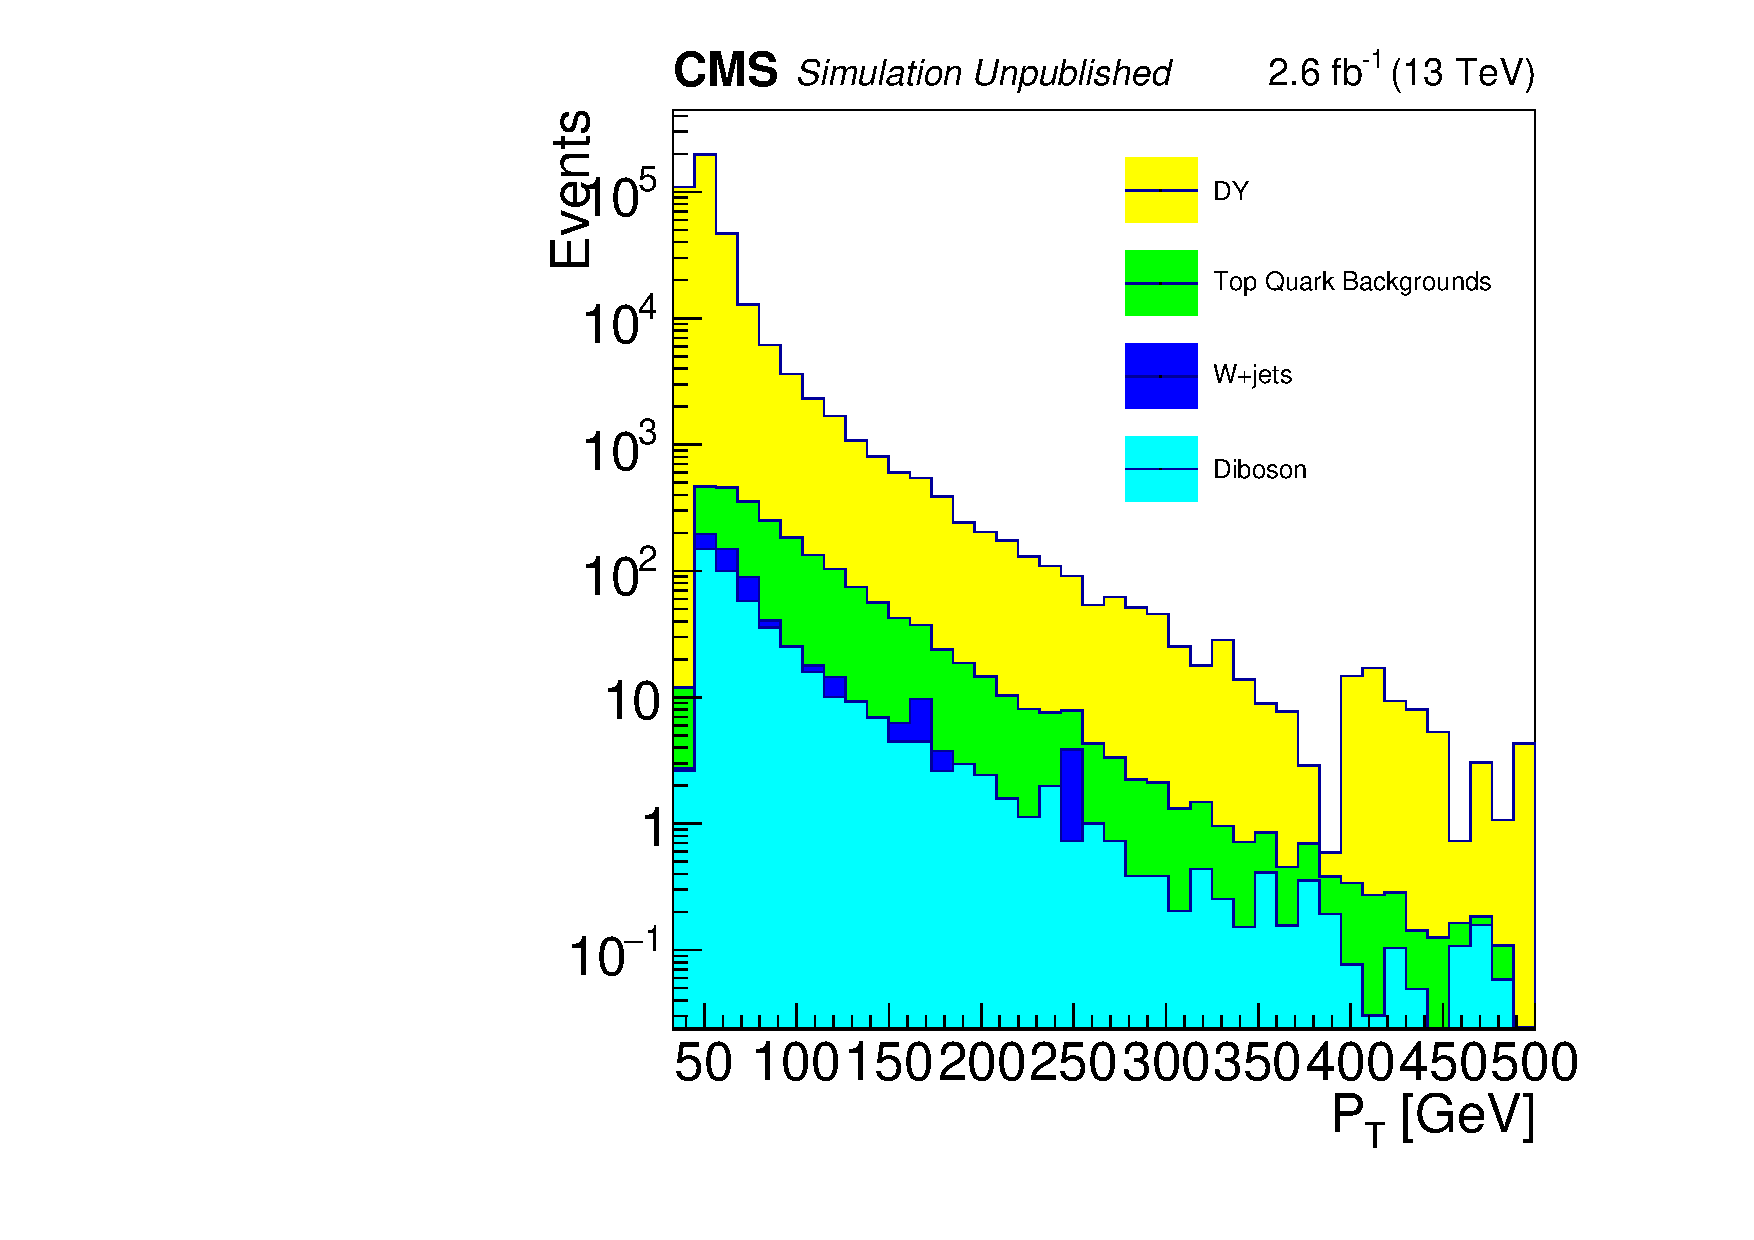
\includegraphics[width=2.4in]{figures/l1_pt_LooseSelection_TwoLeptsAndJets_EEChannelBkgndMC_log.pdf}
		\caption{leading $\pt$ electron}\label{fig:bkgLeptJetPtsa}
	\end{subfigure}
	\thickspace
	\begin{subfigure}[t]{2.4in}
		\centering
		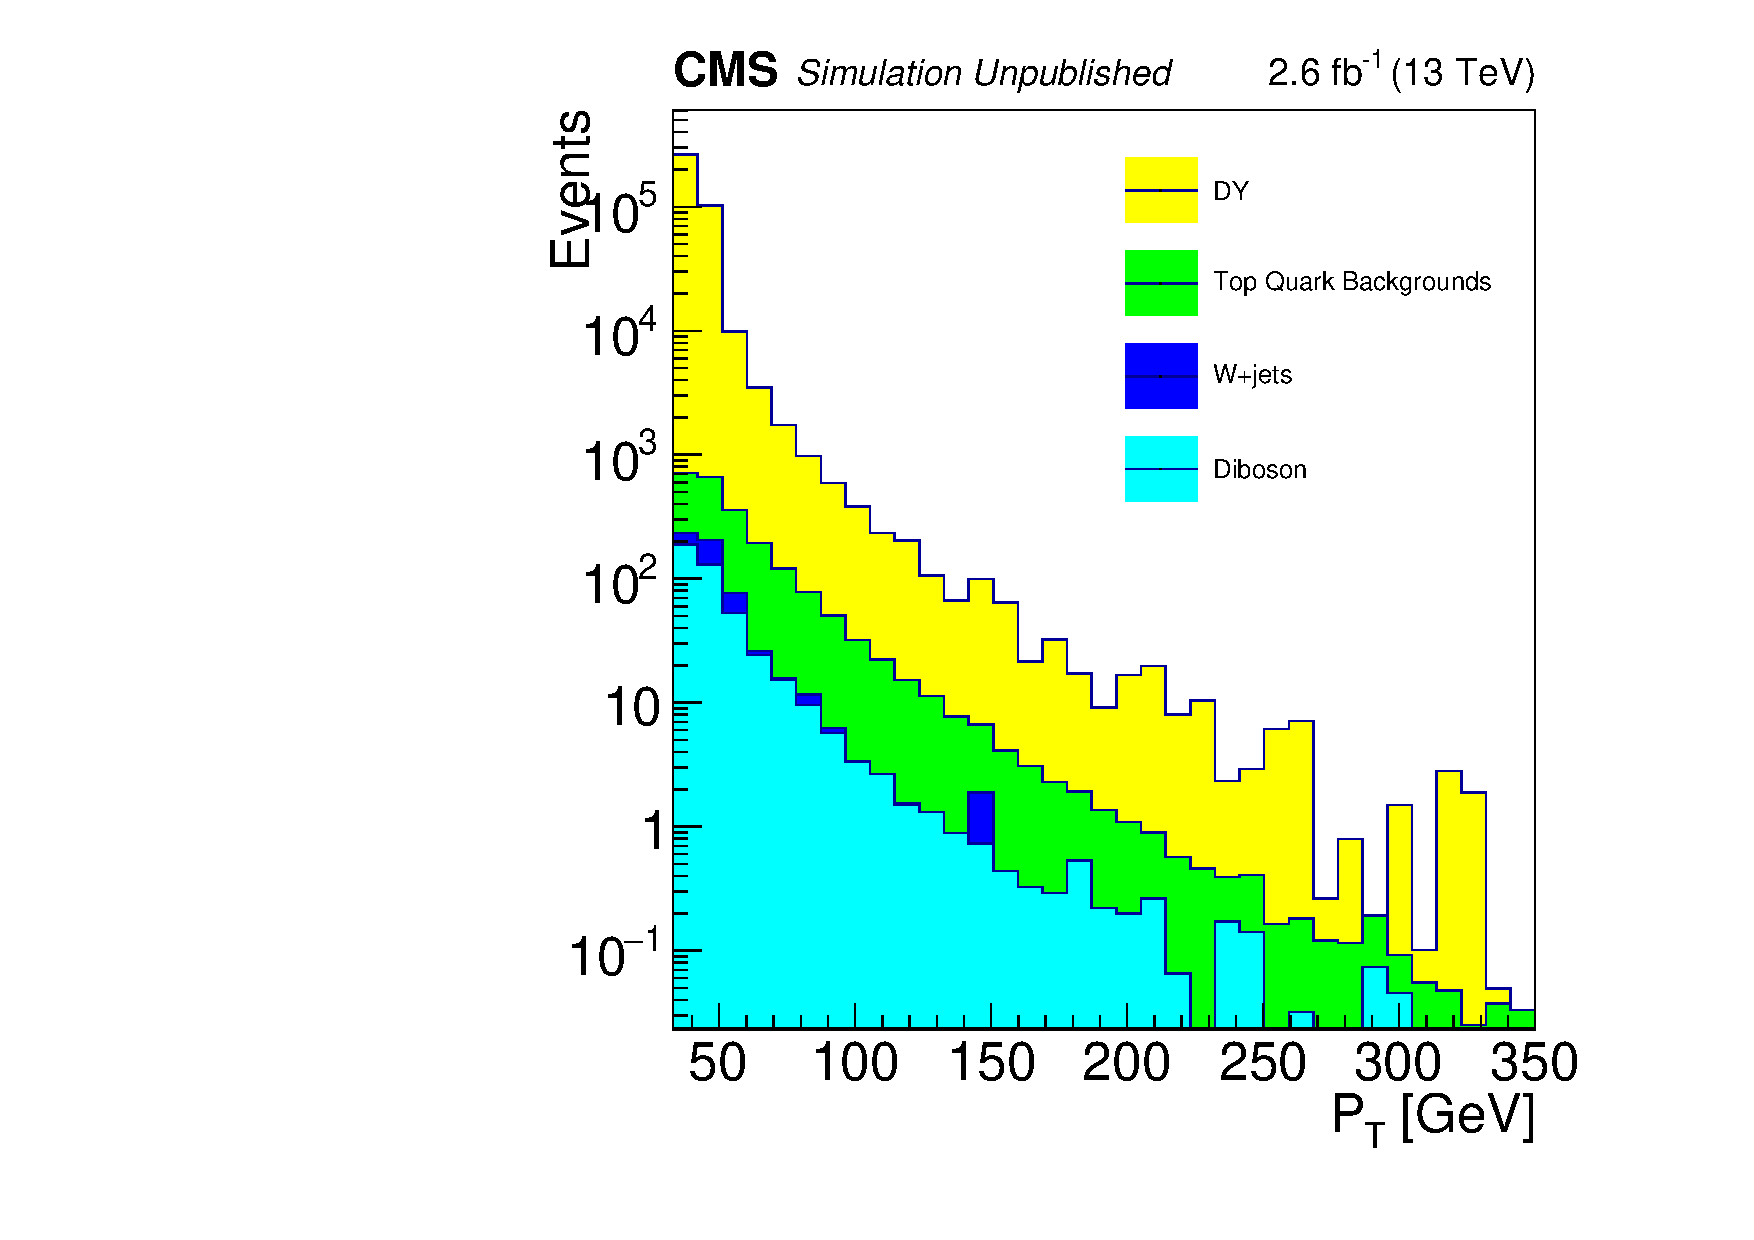
\includegraphics[width=2.4in]{figures/l2_pt_LooseSelection_TwoLeptsAndJets_EEChannelBkgndMC_log.pdf}
		\caption{subleading $\pt$ electron}\label{fig:bkgLeptJetPtsb}
	\end{subfigure}
	\newline
	\newline
	\newline
	\newline
	\begin{subfigure}[t]{2.4in}
		\centering
		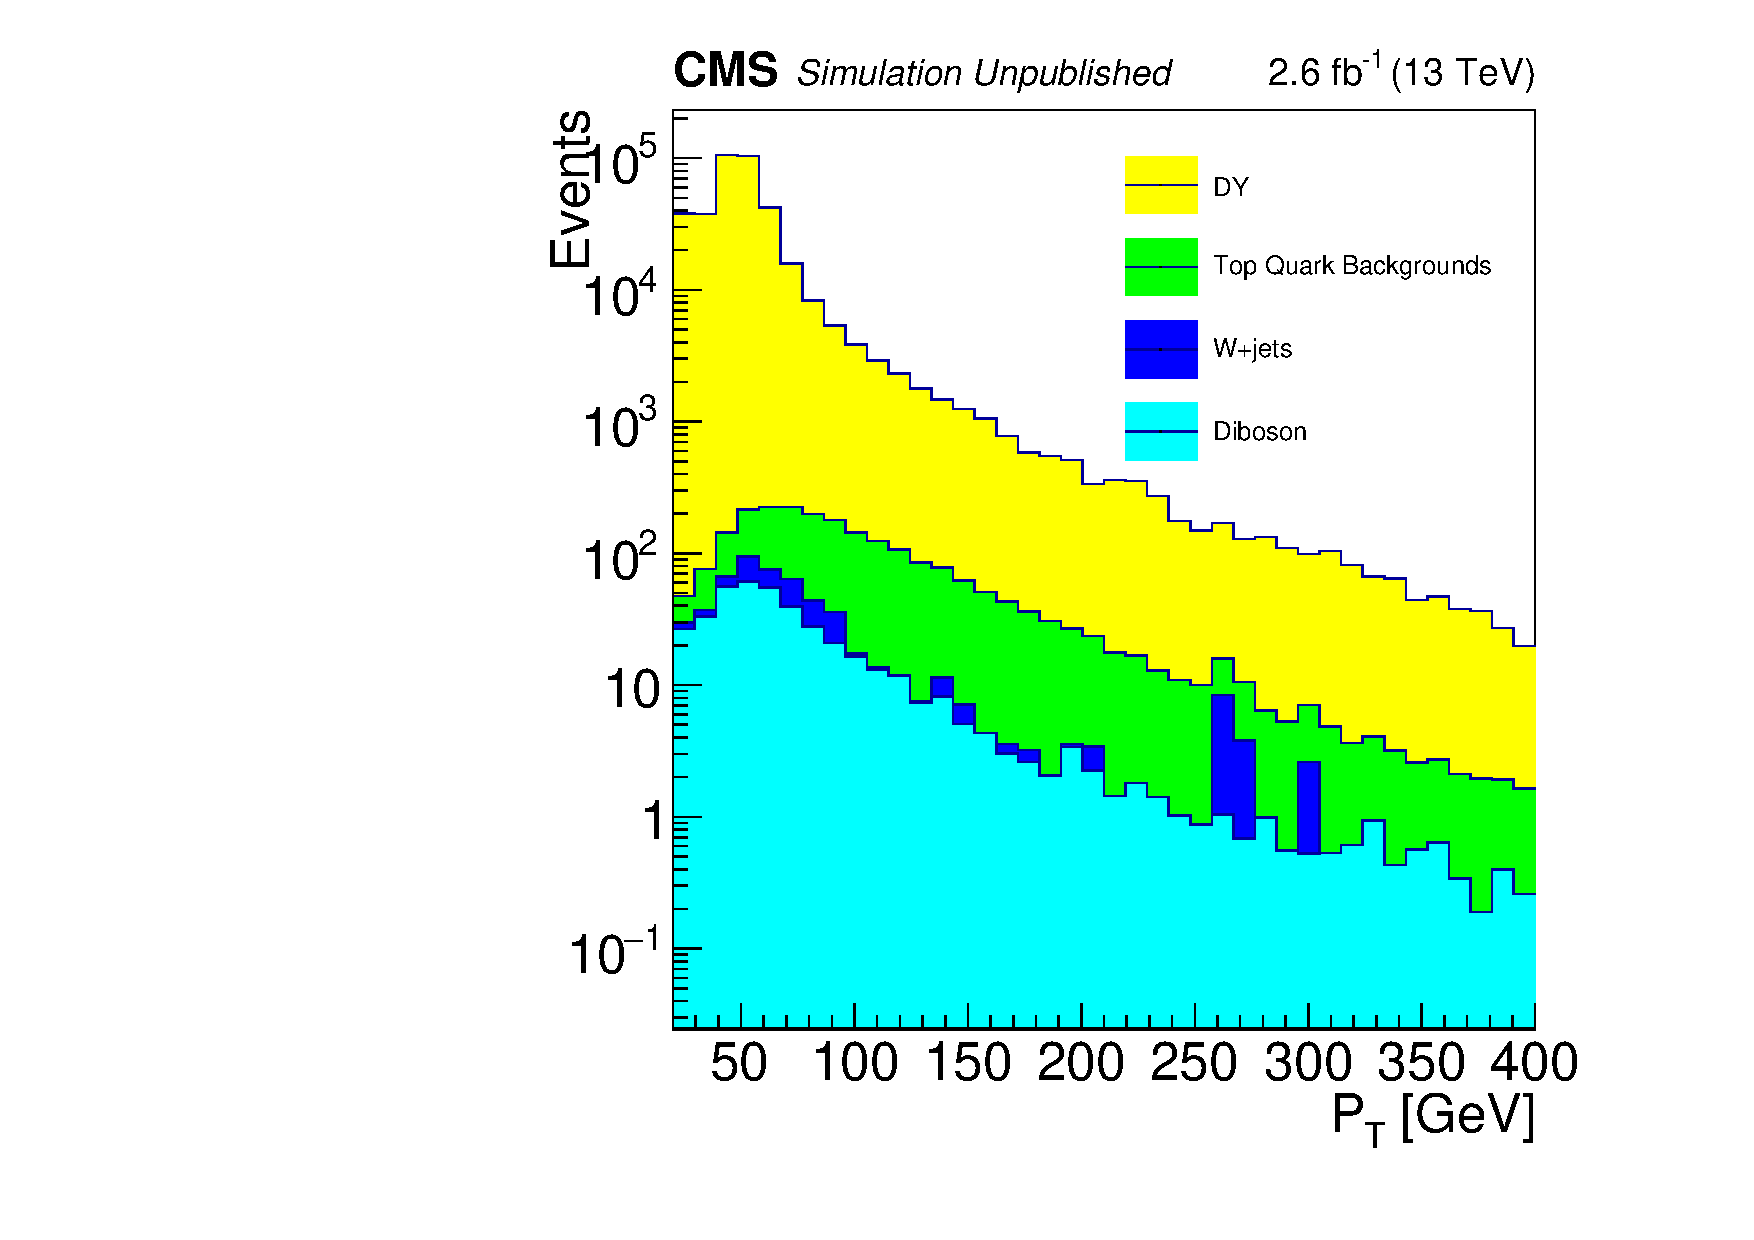
\includegraphics[width=2.4in]{figures/j1_pt_LooseSelection_TwoLeptsAndJets_EEChannelBkgndMC_log.pdf}
		\caption{leading $\pt$ jet}\label{fig:bkgLeptJetPtsc}
	\end{subfigure}
	\thickspace
	\begin{subfigure}[t]{2.4in}
		\centering
		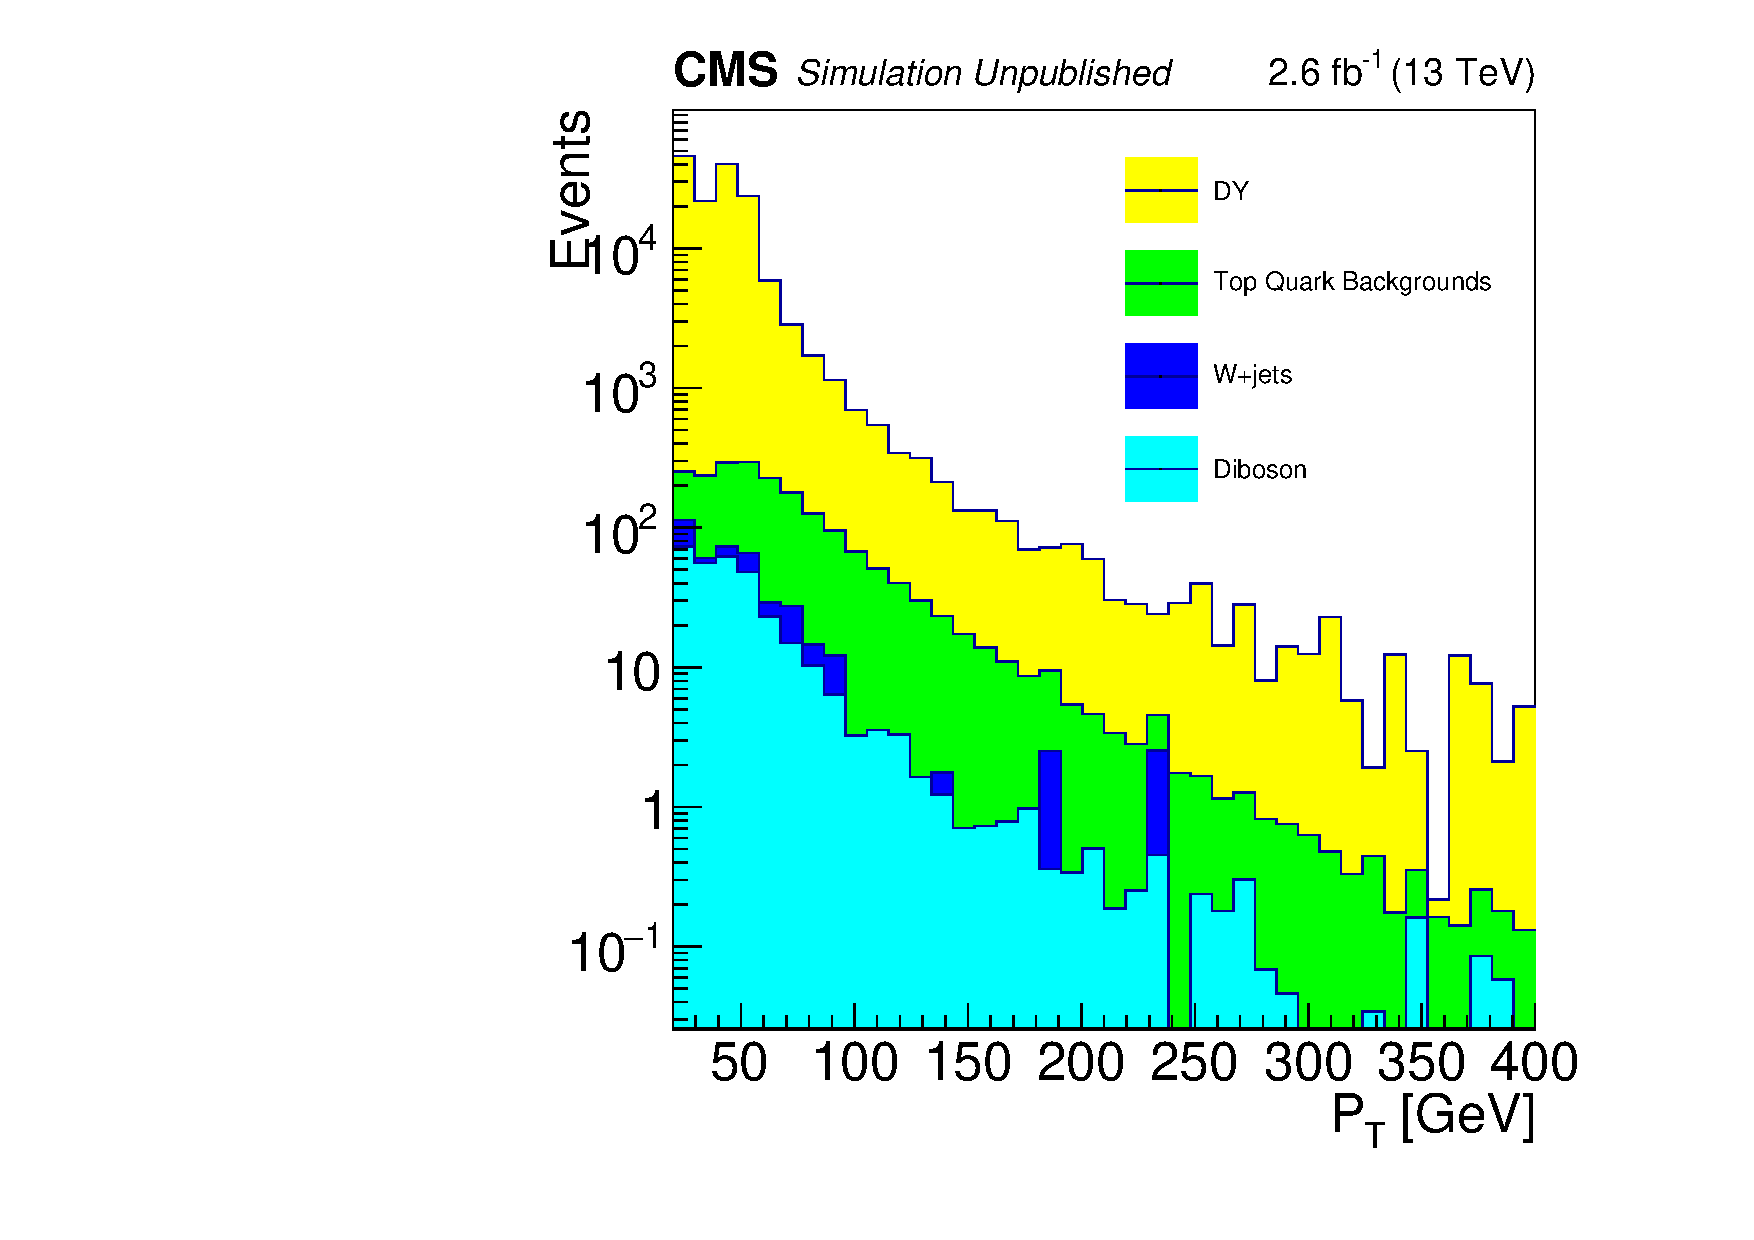
\includegraphics[width=2.4in]{figures/j2_pt_LooseSelection_TwoLeptsAndJets_EEChannelBkgndMC_log.pdf}
		\caption{subleading $\pt$ jet}\label{fig:bkgLeptJetPtsd}
	\end{subfigure}
	\caption{The $\pt$ of electrons and jets reconstructed in simulated background events that passed the $ee$-channel offline ID and 
	full online selection criteria.}\label{fig:bkgLeptJetPts}
\end{figure}


\subsection{Offline Kinematic Selection Criteria}
Differences in lepton and jet kinematics between signal and background events, online lepton selection criteria, and other reasons 
motivated offline lepton and jet kinematic selection criteria.  These reasons and the resulting selection criteria are described here, 
and apply equally to the $eejj$ and $\mu\mu jj$ final states.

The large expected \mWR and the CMS jet $\pt$ resolution motivated the jet $\pt$ and $\eta$ selection criteria.  The \WR is 
expected to be heavy ($\mWR > 3$ $\TeV$), so it is produced with with low momentum.  Therefore the \WR quark decay products are emitted 
uniformly in $\phi$ and $\theta$ relative to the beam axis, and the quarks hadronize into jets in the central $|\eta|$ 
region (Figure \ref{fig:wrLeptJetEtas}).  Thus, each event was required to have two jets reconstructed with $|\eta| < 2.4$.  Also due to 
the large expected \mWR, the jets are produced with large $\pt$ (Figure \ref{fig:wrLeptJetPts}).  However, the $\pt$s of both \WR quarks 
decrease with lower $\mnul/\mWR$ (Figure \ref{fig:wrLeptQrkPtsVarMNu}), so the jet $\pt$ selection threshold should be as low as possible 
to search for low $\mnul/\mWR$ signals.  Jets reconstructed with $|\eta| < 1.3$ and $\pt > 40$ $\GeV$ were measured 
with a $\pt$ resolution of 16\% or better; for $|\eta| < 1.3$ and $30 < \pt < 40$ $\GeV$ the resolution worsened to $\sim$21\% 
\cite{jetResolutionInCollisions}.  To avoid low $\pt$ jets measured with poor $\pt$ resolution, each event was required to have two 
jets passing identification criteria and reconstructed with $|\eta| < 2.4$ and $\pt > 40$ $\GeV$.  If more than 2 jets passed these 
criteria, the two highest $\pt$ jets were used.

%The 40 $\GeV$ threshold was validated by comparing a \WR signal to ST backgrounds.  As listed in Table \ref{tab:lowerJetPtCuts}, 
%reducing the jet $\pt$ threshold reduces sensitivity to a \WR signal relative to ST backgrounds.

%\begin{table}[h]
%	\caption{The signal (S) over background (B) sensitivity, represented by S/$\sqrt{B}$, for different $\pt$ 
%	selection criteria on one jet.  The background is estimated using simulated \DY+jets and $t\bar{t}$ events, and the 
%	signal is estimated using simulated $\WR \rightarrow \mu\mu jj$ events with $\mWR = 2.2 \TeV$ and $\mnul = 1.1 \TeV$.}
%	\label{tab:lowerJetPtCuts}
%	\centering
%	\begin{tabular}{c|c}
%		jet $\pt$ threshold ($\GeV$) & S/$\sqrt{B}$ \\  \hline
%		30 &  12.1  \\
%		40 &  12.6  \\ \hline
%	\end{tabular}
%\end{table}

The large expected \mWR and trigger selection criteria motivated the offline lepton $\pt$ and $\eta$ selection criteria.  For the same 
reason cited for the \WR quarks, the lepton progeny of the \WR are emitted in the central $|\eta|$ region (Figure \ref{fig:wrLeptJetEtas}) 
with high $\pt$ (Figure \ref{fig:wrLeptJetPts}).  Therefore, each event was required to have two leptons reconstructed with $|\eta| < 2.4$ 
and $\pt > 53$.  The $\pt > 53$ requirement is applied to electrons and muons, and the 53 $\GeV$ threshold was used so that both muons 
were selected in a $\pt$ region where the trigger efficiency was maximized.  In \WR decays one lepton is often produced with greater 
$\pt$ than the other, so an additional lepton $\pt$ requirement was applied.  At least one reconstructed lepton was required to have 
$\pt > 60$ $\GeV$ to increase sensitivity to a \WR signal relative to the ST backgrounds (Table \ref{tab:lowerLeptPtCut}).  If more than 
2 leptons passed these criteria, the two highest $\pt$ leptons were used.

\begin{table}[h]
	\caption{The signal (S) over background (B) sensitivity, represented by S/$\sqrt{B}$, for different $\pt$ selection 
		criteria on the leading lepton.  The background is estimated using simulated \DY+jets and $t\bar{t}$ events, and the 
		signal is estimated using simulated $\WR \rightarrow \ell\ell jj$ events with $\mWR = 2.2 \TeV$ and $\mnul = 1.1 \TeV$.}
	\label{tab:lowerLeptPtCut}
	\centering
	\begin{tabular}{c|c}
		$\ell$ $\pt$ threshold ($\GeV$) & S/$\sqrt{B}$ \\  \hline
		53 &  11.7  \\
		60 &  12.6  \\ \hline
	\end{tabular}
\end{table}

Jets are clustered from reconstructed particles using the anti-$k_{T}$ algorithm with distance parameter $R = 0.4$.  For a particle 
separated from a jet's axis by $\Delta R = G$, the distance parameter $R$ weights the likelihood of clustering that particle into the 
jet by $(\frac{0.4}{G})^{2}$.  Thus, the parameter $R$ constrains the maximum distance between a jet constituent and the jet axis.  
However, it is possible for a reconstructed particle to be clustered into a jet and be separated from the jet axis by $\Delta R > 0.4$.  
To avoid selecting a lepton reconstructed near a jet, each reconstructed lepton that passed the identification, $\pt$, and $\eta$ 
selection criteria was required to be separated from both selected jets by $\Delta R > 0.4$.

The \WR decay produces two high $\pt$ leptons whose dilepton mass $\Mll$, given by Equation \ref{eq:dileptMass}, varies with $\mnul/\mWR$.  
For $\mnul/\mWR$ near 1 the decay $\WR \rightarrow \ell_{1}\nul$ produces a \nul nearly at rest, and a $\ell_{1}$ that moves away from the 
\nul.  Subsequently the decay $\nul \rightarrow \ell_{2}jj$ produces a $\ell_{2}$ that moves in a random direction with respect to 
$\ell_{1}$ (Figure \ref{fig:wrLeptAngleSepVarMNu}).  Thus for $\mnul/\mWR$ near 1 the two lepton trajectories are uncorrelated, and the 
$\Mll$ is driven by the square root of the product of the two lepton momentum magnitudes, $\sqrt{|p_{1}||p_{2}|}$.  This variable increases 
with \mWR (Figure \ref{fig:wrLeptSqrtMomMagVarMNu}), so $\Mll$ also increases with \mWR.  As explained earlier, as $\mnul/\mWR$ decreases 
from 1 the \nul carries more energy as momentum, and this increases the $\Mll$ relative to signal hypotheses with $\mnul/\mWR \sim$1 (Figure 
\ref{fig:wrMllVarMNu}).  Thus for a given \mWR hypothesis, the $\Mll$ will be minimized when $\mnul/\mWR \sim$1, and this minimum increases 
with \mWR.  Since a large range of \mWR values were excluded previously \cite{cmsWRRunOneResults}, each event that passed all previous 
selection criteria was required to have two leptons with $\Mll > 200$ $\GeV$.  The 200 $\GeV$ threshold was chosen because a lower threshold 
would increase the backgrounds without a corresponding increase in the signal (Table \ref{tab:lowerMllCut}), and a higher threshold would 
reduce sensitivity to signals with $\mnul/\mWR \sim$1 without a similar reduction in the backgrounds.

\begin{equation}
	\Mll = \sqrt{2|p_{1}||p_{2}|(1\thickspace - \thickspace \cos(\theta_{12}))}
	\label{eq:dileptMass}
\end{equation}

\begin{figure}[h]
	\centering
	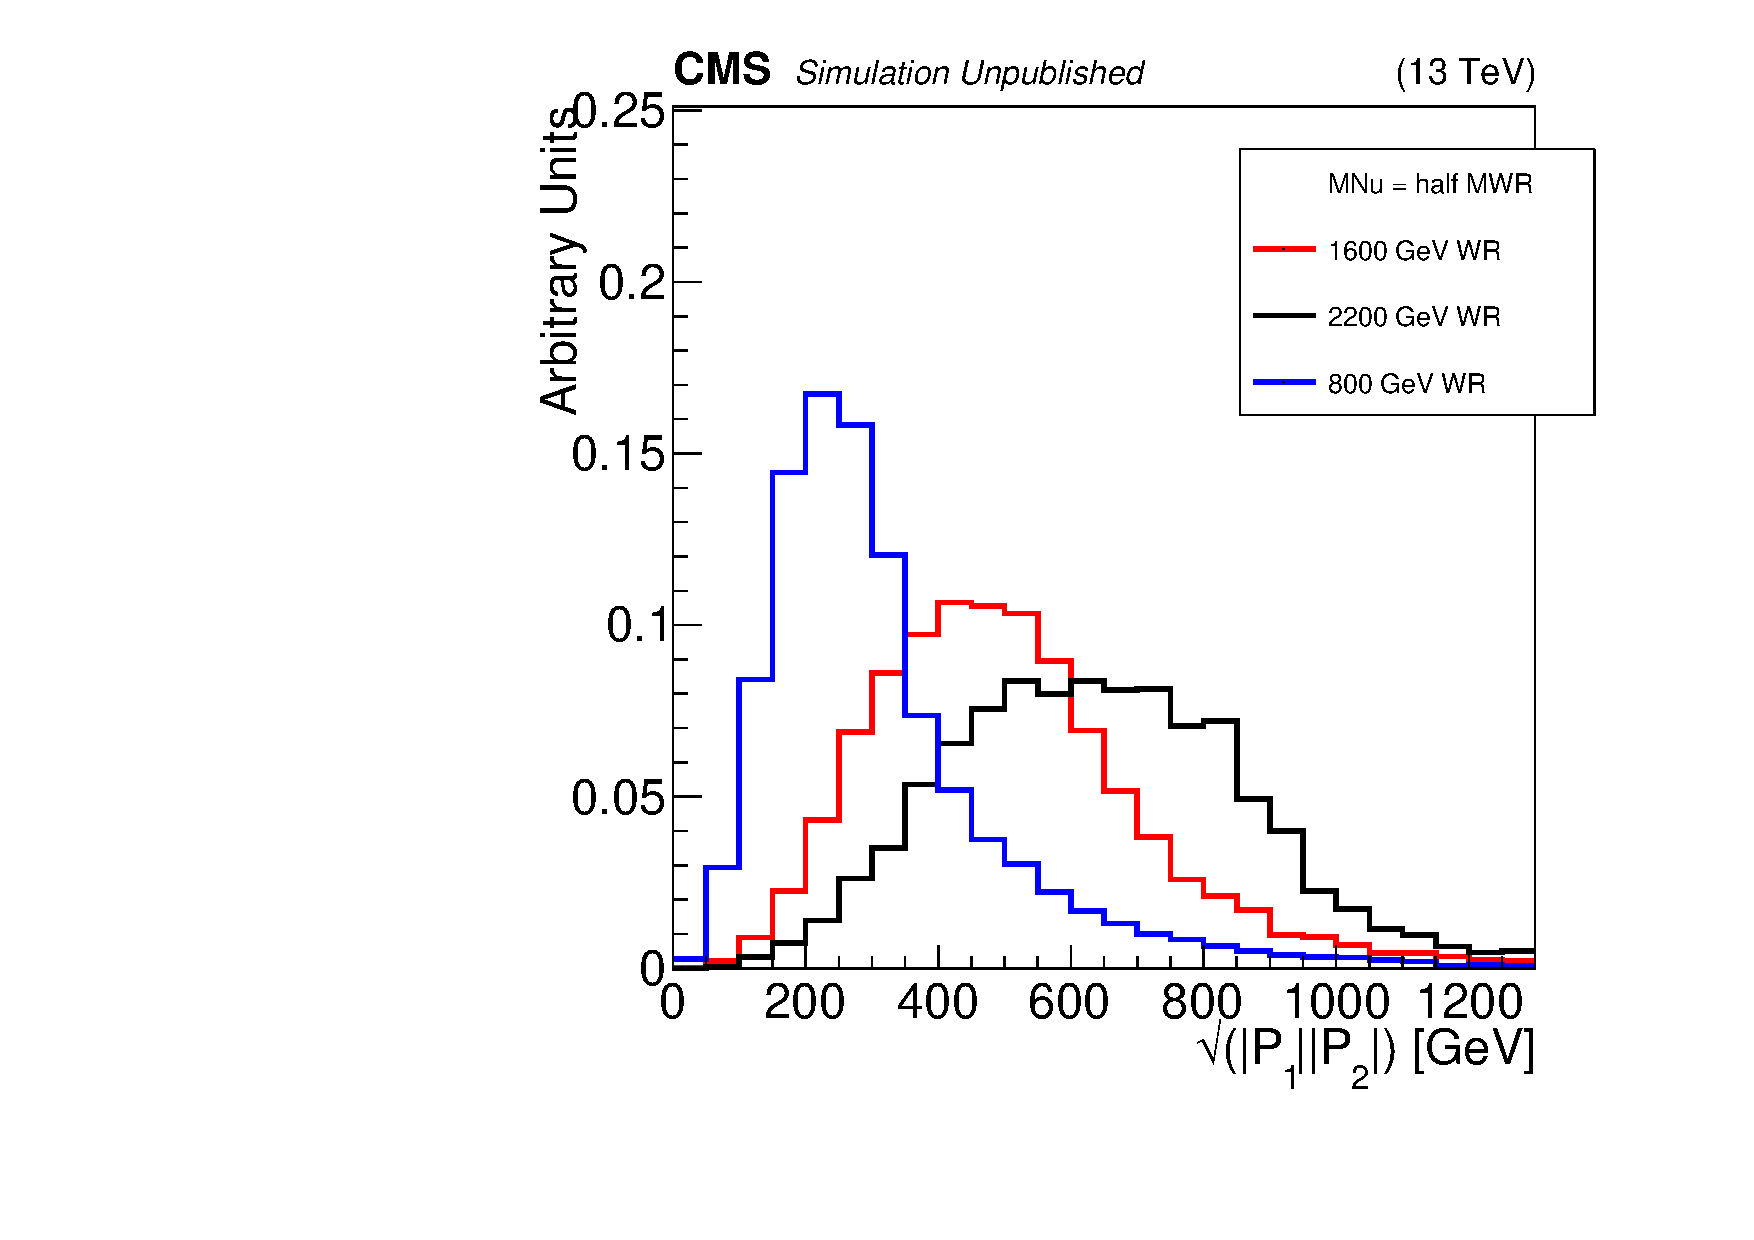
\includegraphics[width=0.5\textwidth]{figures/sqrtProdGenLeptMomentumMag_several_MWR_and_MNu_private.pdf}
	\caption{The square root of the product of the momentum magnitudes of the two leptons produced in $\WR \rightarrow \ell_{1}\ell_{2} qq$ 
		events with several \mWR and $\mnul = \frac{1}{2}\mWR$.}
	\label{fig:wrLeptSqrtMomMagVarMNu}
\end{figure}

\begin{table}[h]
	\caption{The signal (S) over background (B) sensitivity, represented by S/$\sqrt{B}$, for different $\Mll$ selection 
		criteria.  The background is estimated using simulated \DY+jets and $t\bar{t}$ events, and the 
		signal is estimated using simulated $\WR \rightarrow \ell\ell jj$ events with $\mWR = 2.2 \TeV$ and $\mnul = 1.1 \TeV$.}
	\label{tab:lowerMllCut}
	\centering
	\begin{tabular}{c|c}
		$\Mll$ threshold ($\GeV$) & S/$\sqrt{B}$ \\  \hline
		180 &  12.0  \\
		200 &  12.6  \\ \hline
	\end{tabular}
\end{table}

Applying the previous selection criteria to ST background events resulted in a $\Mlljj$ distribution, represented in Figure 
\ref{fig:sculptedMlljj}, that peaked near 500 $\GeV$.  To avoid this peak, each event was required to have $\Mlljj > 600$ $\GeV$.

\begin{figure}[h]
	\centering
	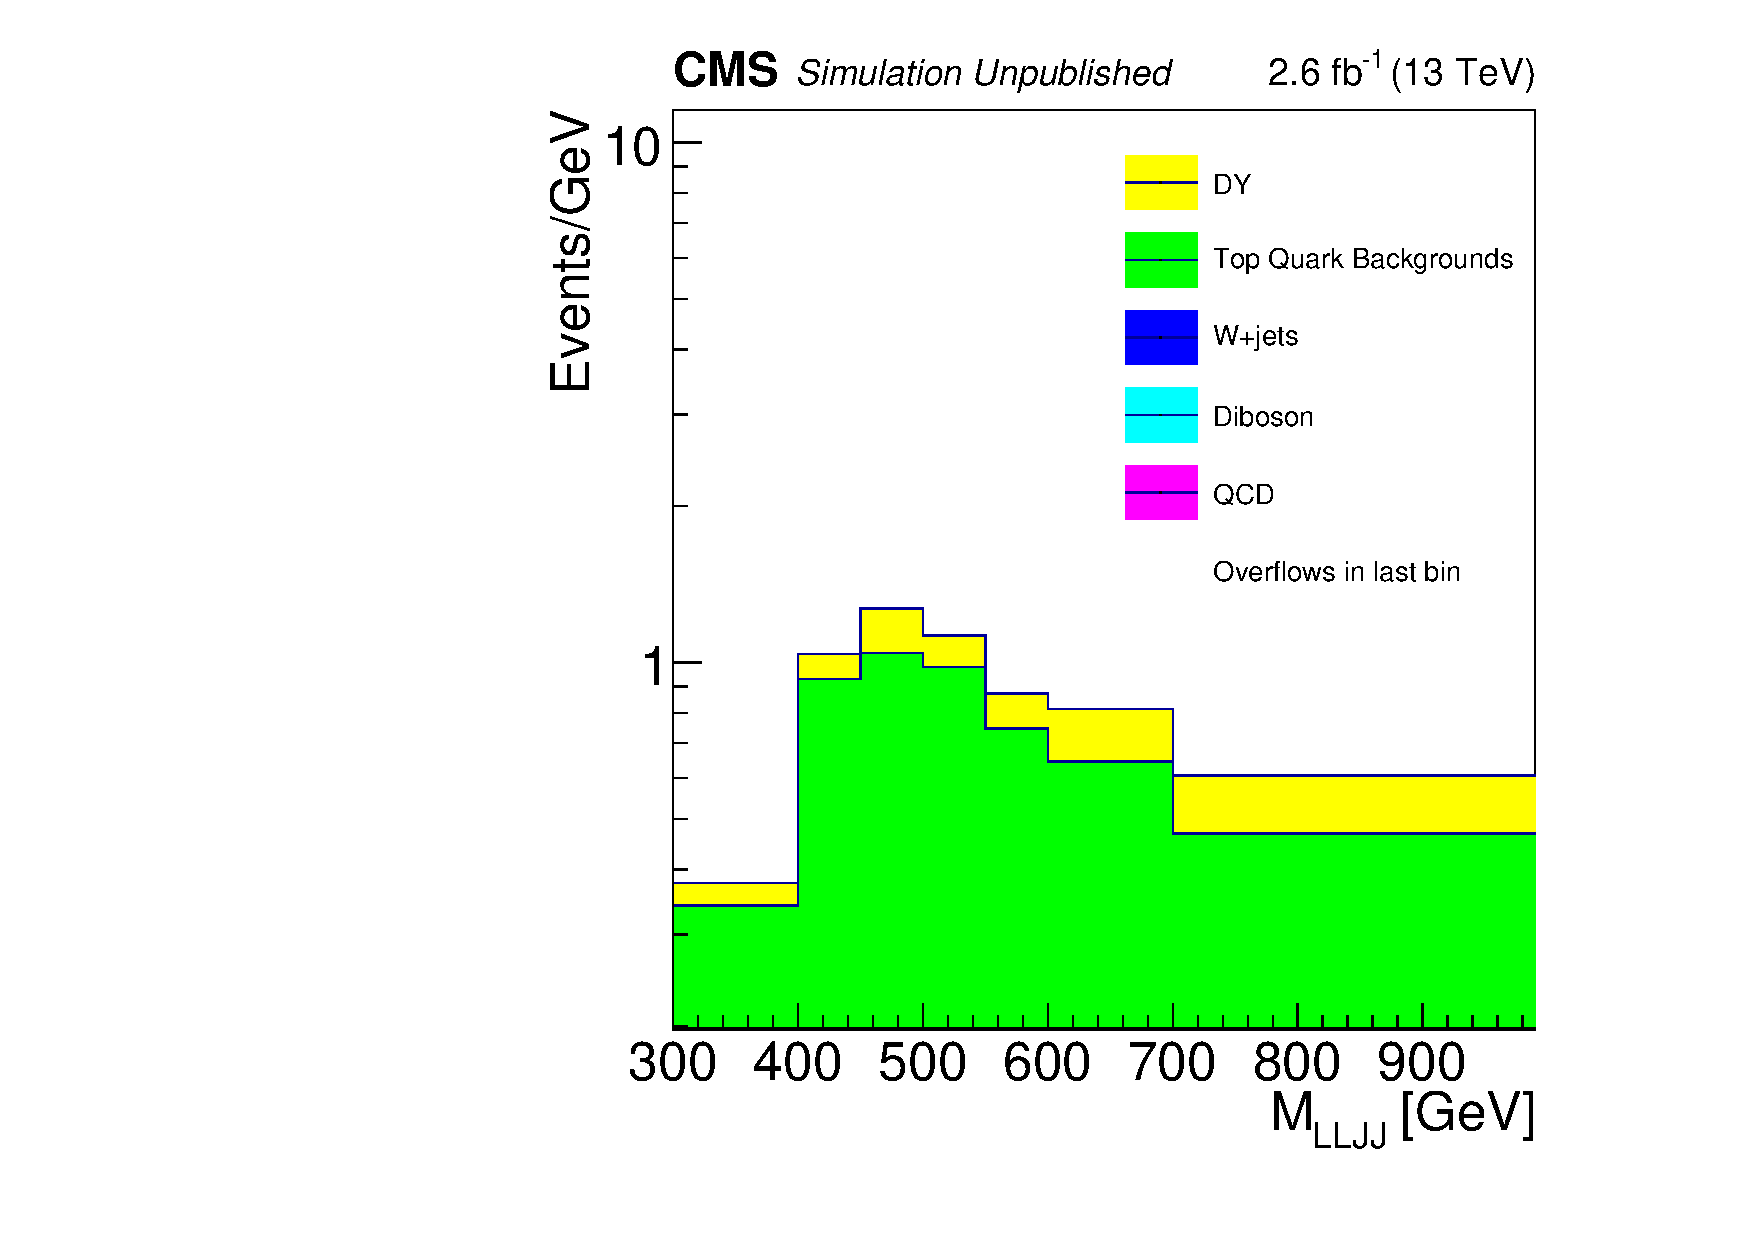
\includegraphics[width=0.5\textwidth]{figures/Mlljj_varBins_SignalRegion_EEChannelBkgndMC_DYMadHTAndIncl_TTBarFromData_log.pdf}
	\caption{The $\Mlljj$ distribution in simulated background events after applying offline kinematic selection criteria.}
	\label{fig:sculptedMlljj}
\end{figure}

The offline kinematic selection criteria are summarized in Table \ref{tab:offlineKinemSel}.  The thresholds 
of the $\Mll$ and $\pt$ selection criteria were set as low as possible to increase selection efficiency for signals with $\mnul/\mWR \sim$ 0 or 1 
without a similar increase in selection efficiency for backgrounds.  At a given \mWR the kinematic effects that lower the signal selection 
efficiency for $\mnul/\mWR \sim$ 0 or 1 are minimized or nearly minimized for $\mnul/\mWR = \frac{1}{2}$ (Figure \ref{fig:wrOffSelEffVarMWrMNu}).  
For this reason simulated signal events with $\mnul/\mWR = \frac{1}{2}$ were used to estimate the signal selection efficiency versus \mWR.  The 
net efficiency of online and offline selection criteria versus \mWR, Figure \ref{fig:wrRecoSelectionEff}, exceeded 50\% in the $ee$-channel and 
70\% in the $\mu\mu$-channel.  The efficiency was lower in the $ee$-channel due to the ECAL gap in electron detection for $1.44 < |\eta| < 1.57$, 
and lower efficiency offline ID selection criteria applied to electrons relative to muons.

\begin{table}[h]
	\caption{The kinematic selection criteria applied to reconstructed leptons and jets that passed the offline identification 
	selection criteria.  The criteria were applied in the order that they are listed.}
	\label{tab:offlineKinemSel}
	\centering
	\begin{tabular}{c|c}
		requirement on & threshold  \\  \hline
		lead jet $\pt,\eta$ & $\pt>40\GeV,|\eta|<2.4$ \\
		sublead jet $\pt,\eta$ & $\pt>40\GeV,|\eta|<2.4$ \\
		lead $\ell$ $\pt,\eta$ & $\pt>60\GeV,|\eta|<2.4$ \\
		sublead $\ell$ $\pt,\eta$ & $\pt>53\GeV,|\eta|<2.4$ \\
		$\Delta R(\ell,j)$ & $>0.4$ \\
		$\Mll$ & $>200\GeV$ \\
		$\Mlljj$ & $>600\GeV$ \\ \hline
	\end{tabular}
\end{table}

\begin{figure}[h]
	\centering
	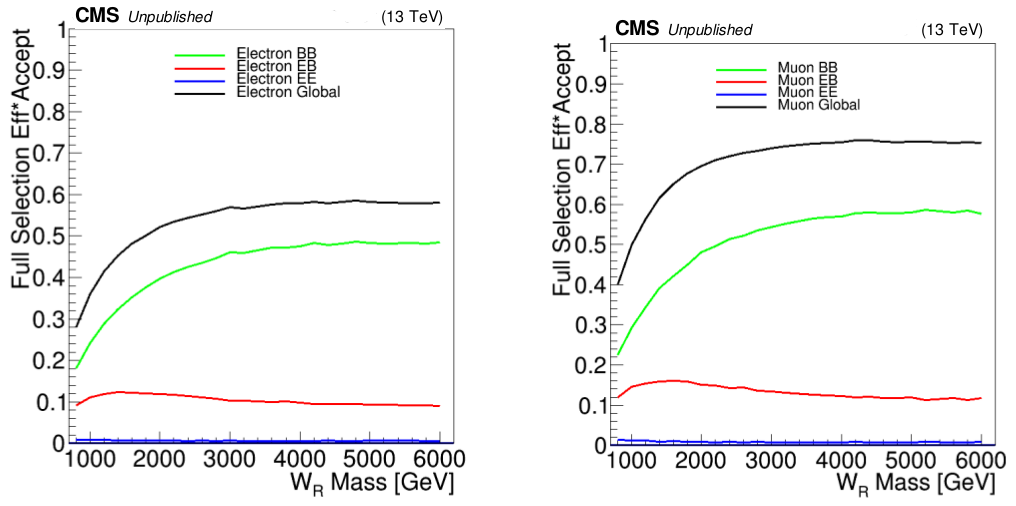
\includegraphics[width=1.0\textwidth]{figures/wrRecoSelectionEfficiency.png}
	\caption{The full selection efficiency in simulated $\WR \rightarrow \ell\ell jj$ events, in the $ee$-channel ($\mu\mu$-channel) 
		on the left (right).  Different curves represent events where both leptons are in the barrel (BB), one was in the 
	endcap (EB), or both were in the endcap (EE).}
	\label{fig:wrRecoSelectionEff}
\end{figure}

\begin{figure}[h]
	\centering
	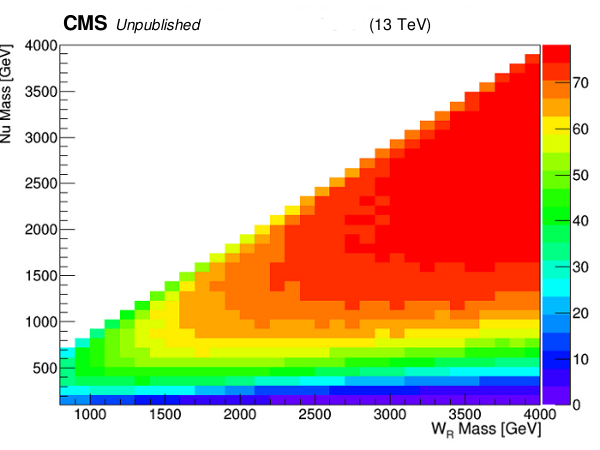
\includegraphics[width=0.5\textwidth]{figures/genWrMuMuAccEff_NoMassWindows13TeV.png}
	\caption{The offline kinematic selection efficiency (\%) in signal events as a function of \mWR and \mnul.}
	\label{fig:wrOffSelEffVarMWrMNu}
\end{figure}


\section{Conclusion}
\label{sec:recoConclusion}
Electrons, muons and jets expected from \WR and \nul decays are reconstructed from signals measured in CMS sub-detectors using dedicated 
reconstruction algorithms.  These algorithms reconstruct leptons, hadrons and jets with high efficiency by using minimal selection criteria, 
and occasionally ($\sim$1-3\%) reconstruct individual particles and jets as the wrong type of particle.  The contribution of incorrectly 
reconstructed particles to $\ell\ell jj$ events was reduced by requiring leptons and jets to pass identification (ID) selection criteria.  
Selected particles were then required to pass kinematic selection criteria to identify reconstructed particles measured with good energy 
resolution that are consistent with \WR decay kinematics.  All selection criteria were applied to data events, and selected events were 
used to make a $\Mlljj$ distribution.  The decay $\WR \rightarrow \ell\ell jj$ transfers all energy of the \WR into the invariant mass of 
the leptons and jets, so evidence of a \WR, independent of \mnul, was searched for as an excess of data events above predicted backgrounds 
in the $\Mlljj$ distribution.  The $\Mlljj$ distribution of the backgrounds was predicted using data and simulated events in control regions 
with no signal contamination.


%%%%%%%%%%%%%%%%%%%%%%%%%%%%%%%%%%%%%%%%%%%%%%%%%%%%%%%%%%%%%%%%%%%%%%%%%%%%%%%%
